%\documentclass[a4paper, traditabstract]{aa} 
\documentclass[twocolumn, traditabstract]{aa}  

%\pdfoutput=1
\usepackage{fixltx2e}
\usepackage[english]{babel}
\usepackage{graphicx,amsmath}
\usepackage{epstopdf}
\usepackage{epsf,color}
\usepackage[mathscr]{eucal}
\usepackage{amsmath}
\usepackage{amssymb,amsfonts}
\usepackage{natbib}
\usepackage{graphicx}
\usepackage{txfonts}
\usepackage{dsfont}
\definecolor{Mygreen}{rgb}{0.00, 0.72, 0.0}
\definecolor{Mypink}{rgb}{1.0, 0.0, 0.5}
\usepackage[breaklinks, citecolor=blue, linkcolor=Mygreen, urlcolor=Mypink, colorlinks=true, debug, baseurl=' ']{hyperref}
\usepackage{float}
\usepackage{color}
\usepackage{scrextend}
\usepackage{nccmath}
\usepackage{mathtools, cuted}
\usepackage{lscape}


\definecolor{Mygreen}{rgb}{0.00, 0.72, 0.0}
\definecolor{Mypink}{rgb}{1.0, 0.0, 0.5}
\definecolor{Blue}{rgb}{0.,0.,1.}
\definecolor{LightSkyBlue}{rgb}{0.691,0.827,1.}
\definecolor{Red}{rgb}{1.,0.,0.}
\definecolor{Green}{rgb}{0.,1.,0.}
\definecolor{Purple}{rgb}{0.5, 0., 0.5}
\definecolor{Try}{rgb}{0.15,0.,1}
\definecolor{Black}{rgb}{0., 0., 0.}

\newcommand{\nika}{{\it NIKA}}
\newcommand{\nikad}{{\it NIKA2}}
\newcommand{\nico}{\color{Mypink}}
%\usepackage{lipsum, color}

%\DeclareSIUnit\parsec{pc}
%\DeclareSIUnit\erg{erg}
%\DeclareSIUnit\deg{deg^{-2}}
%\DeclareSIUnit\count{cnt}

\def\intk#1{\displaystyle\int\frac{d^2k_{#1}}{(2\pi)^2}}
\def\intr#1{\displaystyle\int d^2r_{#1}}
\def\simlt{\lower.5ex\hbox{$\; \buildrel < \over \sim \;$}}
\def\simgt{\lower.5ex\hbox{$\; \buildrel > \over \sim \;$}}
\def\NIKA{\textit{NIKA}}
\def\Skydip{\textit{Skydip}}

\bibpunct{(}{)}{;}{a}{}{,}

\bibliographystyle{aa}

\begin{document}

\title{Polarimetry at millimeter wavelengths with the \nika\ camera: calibration  and performance.}
\author{TBD}
\institute{
Laboratoire de Physique Subatomique et Cosmologie, Universit\'{e} Grenoble-Alpes, CNRS/IN2P3, 53, rue des Martyrs, 38026 Grenoble Cedex, France
}

%\input{}
\date{Received \today \ / Accepted --}
	
\abstract{{\it Herschel} satellite observations have unveiled filamentary
  structures as the preferential sites of star formation. Complementary low
  resolution observations of dust polarization by the {\it Planck} satellite
  {\nico have} demonstrated that these filamentary structures are associated to
  well organised magnetic fields {\nico that} should thus play a major role in
  star formation. A better understanding of this process requires detailed
  observations of galactic dust polarization {\nico on} scales of 0.01 to 0.1
  pc.  Such high resolution polarization observations can be carried out at the
  IRAM 30 telescope using the recently installed \nikad\ camera, which features
  two {\nico frequency bands at 260 and 160 GHz (respectively 1.25 and 2.05 mm),
    the 160~GHz band being polarization sensitive. \nikad\ has its focal plane
    filled with 3500 detectors, its full width half maximum resolutions are 12
    and 18 arsec at 1.25 and 2.05mm respectively and its field of view has a 6.5
    arcmin diameter}.  The \nika\ camera, which consists of two arrays of 132
  and 224 LEKIDs (Lumped Element Kinetic Inductance Detectors) at 1.25 and
  2.05~mm, {\nico **} operated at the IRAM 30 telescope from 2012 to 2015 as a
  test-bench for \nikad. \nika\ was equipped of a room temperature polarization
  system (a multi-layer half wave plate (HWP) and a grid polarizer facing the
  \nika\ cryostat window){\nico . The fast and continuous rotation of the HWP}
  permits the {\nico quasi} simultaneous reconstruction of the three Stokes
  parameters, I, Q and U at 150 and 260 GHz. This paper aims at discussing the
  polarization performances of the \nika\ camera and the pertinence of the choice
  of the polarization setup in the perspective of \nikad.  We also discuss the
  polarised data reduction pipeline that has been specifically developed for
  this project and how systematic effects are dealt with.  We present results on
  compact and extended sources obtained during the February 2015 {\nico technical}
  campaign. These results demonstrate a good understanding of polarization
  systematics and state-of-the-art performance in terms of photometry,
  polarization degree and polarization angle reconstruction.}
%In particular we observe a good agreement comparing the measurement of the calibrator 3C 286 polarization angle at 1.25 mm and 2.05 mm, respectively, $\psi$ = (29.0 $\pm$ 3.9)$^\circ$ and $\psi$ = (27.7 $\pm$ 3.9)$^\circ$ with other experiments observing at millimeter wavelengths. 
%previous studies effectuated by XPol, which give $\alpha\rm_{Sky}$ = [37.3$\pm$0.8]$^\circ$ at 3 mm and $\alpha\rm_{Sky}$ = [33.1$\pm$5.7]$^\circ$ at 1.3 mm.
%For the strong and variable quasar 3C279 we found an agreement with recent observations by CARMA at 1.3 mm, the polarization angles are $\psi$ = (35.9 $\pm$ 3.2)$^\circ$ and $\psi$ = (31.9 $\pm$ 3.6)$^\circ$ at 1.25 mm and 2.05 mm, respectively.
%We also observed known extended sources: Crab nebula, Orion-OMC1, M87 and Cygnus A. The averaged angle of the Crab nebula  measured where the polarization intensity $IPOL$ is bigger than 0.1 Jy/beam is $\alpha_{\rm Sky}$ = 143.7 $\pm$ 14.7 $^\circ$ at 150 GHz. The measured averaged polarization angle measured by {\it NIKA} in the OMC1 region of the Orion molecular cloud is $\psi$ = (21.3 $\pm$ 3.6)$^\circ$ and  $\psi$ = (22.1 $\pm$ 2.6)$^\circ$ at 2.05 and 1.25 mm, respectively, in agreement with Polka instrument observations.}
	
\authorrunning{TBD}
\keywords{Techniques: polarization -- KIDs --  individual: NIKA }
\maketitle

{\nico
\begin{itemize}
\item a few typos
\item changed polarisation into polarization
\item ** when i removed a word
\item we must try to relocate the plots, I know it can be hopeless though...
\item we need to harmonize the measured FWHM's
\item Leakage as seen by BICEP et al to be checked and/or *a bit* more
  discussed.
\item residual instrumental polarization
\item bien insister que c'etait un run technique, qu'on continue \`a investiguer
  les sources de syst\'es et comment les traiter au mieux, sinon on va se faire
  \'etrier sur le bruit non gaussien et les choses incomprises encore comme les
  angles des quasars.
\end{itemize}
} 

\section{Introduction}\label{sec:introduction}
Magnetic fields have been proved to play a predominant role in a large number of
astrophysical processes from galactic to cosmological scales. In particular,
recent observations with the {\nico {\it Herschel} and {\it Planck}} \citep{planck2013mission}
satellites have provided us with complete, sensitive maps of the star forming
complexes in the galaxy. These maps reveal large scale filamentary structures as
the preferential sites of star formation
\citep{2010A&A...518L.100M,2010A&A...518L.102A}. These filamentary structures
are associated to organised magnetic field topology at scales larger than 0.5 pc
\citep{2014prpl.conf...27A}. This indicates that magnetic field may play a major
role in star formation and that they need to be explored in details in scales of
0.01 to 0.1 pc \citep{2014prpl.conf...27A}.{\nico we start by saying ``have been
  proved'' and we end by ``may play a role''...}

At millimeter and sub-millimeter wavelengths the magnetic field orientation can
be explored using the polarized thermal dust emission
\citep{2015A&A...576A.104P,2016arXiv160100546P}. Dust grains are more generally
prolates and tend to partially align their major axis orthogonally to the
magnetic field lines \citep{1951ApJ...114..206D, 1988QJRAS..29..327H}. As they
mainly {\nico emit} along their major axis, this results into coherently
polarized dust emission in the plane perpendicular to the magnetic field
lines. Thus, polarized dust emission permits to recover the direction of the
magnetic field lines projected on the plane of the sky
\citep{2015A&A...576A.106P}. The {\it Planck} satellite has mapped the polarized
dust emission at 353 GHz on large angular scales over the entire sky
\citep{2014A&A...571A...8P,2015arXiv150201587P}{\nico, and favors} a high degree
of polarization, up 15 \% \citep{planckdust}, confirming previous {\it Archeops}
results \citep{2004A&A...424..571B}{\nico. This opens} a new window on the
understanding of galactic magnetic fields.

Unfortunately, the {\nico ** 5 arcmin resolution} of the {\it
  Planck} 353~GHz data limits the study of the galactic magnetic field to scales
of 0.2 to 0.5 pc even for the closest clouds. For a detailed exploration of the
magnetic field lines in the star forming filamentary structures (scales of 0.01
to 0.1 pc) we need to {\nico foresee} high resolution observations (10-20 arcsec
resolution) of the polarized dust emission \citep{2014prpl.conf...27A}.

The \nikad\ dual band millimeter camera \citep{2016arXiv160102774C}, recently
(October 2015) installed at the IRAM 30 m telescope in Pico Veleta (Spain), is
particularly well adapted {\nico to} such high resolution observations of the
polarized thermal dust emission.  \nikad\ features two frequency bands at 260
(polarized) and 160 (non polarized) GHz for a total of 3500 LEKID (Lumped
Element Kinetic Inductance Detector) detectors{\nico. \nikad\ has a 12
  (resp.~18) arcsec full width half maximum resolution at 260~GHz
  (resp.~160~GHz) and a 6.5 arcmin diameter field-of-view (FOV) at both
  frequencies}. Between 2012 and 2015 a reduced version of \nikad\, named
\nika\ \citep{monfardini2010,catalano2014}, has been operated at the IRAM 30 m
telescope as a test-bench. \nika\ was also a dual band camera at 150 and 260 GHz
with a total of 300 LEKID, 12 and 18 arcsec resolution, {\nico but a 1.8~arcmin diameter}
FOV. Thanks to a specifically designed polarization setup \nika\ has provided
polarized observations at both frequency bands \citep{2015JLTP..tmp...76R}. This
polarization setup includes an analyser and a half-wave plate (HWP).

Experiments such as Planck \citep{planck_mission}, BICEP \citep{bicep}, ACTPol
\citep{ACTPOL}, QUaD \citep{QUAD}, QUIET \citep{QUIET}, QUIJOTE \citep{QUIJOTE},
rotate the instrument w.r.t. the sky. This modulates the input polarization
signal {\nico providing the required angular coverage to reconstruct the I, Q
  and U Stokes parameters}. By contrast, {\nico other experiments rotate a HWP
  in front of an analyser to modulate the incoming sky polarization. PILOT
  \citep{PILOT} and SPIDER \citep{SPIDER} change the HWP orientation step by
  step and maintain it fixed during some periods of observation. EBEX
  \citep{ebex}, POLARBEAR \citep{polarbear}, BLASTPol \citep{BLASTPol} and
  \nika-\nikad\ take another option that is to rotate the HWP continuously}. We
  discuss in this paper the polarization performance of the \nika\ camera and
  the implications for the \nikad\ design.

%recent {\it Herschel} satellite observations have unveiled filamentary structures as the preferential sites of star formation. 
%Complementary low resolution observations of dust polarization by the {\it Planck} satellite has demonstrated that these filamentary structures are associated to well organised magnetic fields, which should thus play a major role in star formation. A better understanding of this process requires detailed observations of galactic dust polarization in scales of 0.01 to 0.1 pc

%The continuum emission observed at submm wavelengths is mainly due to the thermal emission of prolate dust grains which partially align 
%eading to significant polarized emission.
	
%	Since it governs a number of physical and chemical processes in the interstellar medium (ISM), interstellar dust plays a key role in the Milky Way. With a pressure comparable to thermal gas and cosmic rays, the Galactic magnetic field plays a crucial role in our Galaxy \citep{planckdust}.
	
%	Dust polarization observations can be used to define the magnetic field direction projected onto the plane of sky, thus complementing our knowledge of the Galactic magnetic field, obtained via measurements of Faraday rotation, synchrotron emission and Zeeman splitting \citep{crutcher2010}.
%	Magnetic fields provide the pressure balance required to support the ISM against gravitational collapse on large scales, regulating the filamentary structures
%Observations at far-infrared and sub-millimeter wavelengths have demonstrated that the thermal emission from dust grains is often partially polarized \citep{schle1998, brenda2000}, which is usually attributed to the partial alignment of the emitting grains by magnetic field. 

 %PLANCK large-scale polarization maps at 353 GHz show a polarized thermal dust emission coming from the elongated grains aligned with the magnetic field. The dust polarization fraction $p$ is observed to range from zero to more than 15 $\%$ \citep{planckdust}. These observations open the field for many detailed studies.
%While PLANCK satellite provide polarization information on large scales ($> 5'$ or $> 0.2$ pc in the nearest clouds) between 0.85 mm and 3 mm, only higher resolution instrument such as {\it NIKA} can probe the critical $\sim 0.01 - 0.05 $ pc scales ($\sim$ 10"-60" in the nearest clouds) at which magnetic field lines may channel the matter of interstellar filaments into growing dense cores.

%Since the role of the magnetic fields in regulating grain alignment and filamentary structures observed within molecular clouds remains not well understood \citep{Fiege2000}; polarization high angular resolution observations provided by {\it NIKA} polarimeter and the following \nikad\ instrument could be probe this role. 
%One of the challenges of the modern millimeter and sub-millimeter astronomy is to observe Galactic regions in polarimetry in order to investigate this role.
%Since the degree of dust continuum polarized emission is low (typically ~ 5$\%$ - \citep{Matthews2002}), a systematic polarimetric study of nearby star-forming filaments and pre-stellar cores requires a fast mapping speed, a high resolution and a large FoV (Field of View) foreseen in {\it NIKA} prototype and improved in the final instrument {\it NIKA}2.

%The {\it NIKA} camera installed until February 2015 at the IRAM 30 m telescope in the Sierra Nevada (Spain) and replaced by {\it NIKA}2 on October 2015 has demonstrated its competitiveness in total power observations \citep{catalano2014, adam2014, adam2015}.
%The observation of the dust emission of Galactic regions is the purpose of the {\it NIKA} polarimeter, consisting of a warm system (300K) composed by a multi-layer Half Wave Plate (HWP) and a polarizer, placed in front of the cryostat window. 

%The fast rotating HWP ($\sim$ 3 Hz ) combined to the small time constant of the Kinetic Inductance Detectors (KIDs) ($ < $ 1 ms) allows to shift the polarized signal at four times the HWP mechanical rotation frequency $\omega$ far from the 1/f noise component. This detection strategy permits the quasi simultaneous measurement of the three Stokes parameters, $I$, $Q$, $U$ on a same area of the Sky \citep{johnson2007}. 


%This paper aims to discuss the performance of the polarization system chosen.
The paper is organised as follows, section ~\ref{nika instrument} presents the
\nika\ instrument and the polarization
setup. Section~\ref{sec:lab_characterisation} discusses the laboratory
characterisation of the polarization instrument. Sect.~\ref{data_analysis}
presents the observational strategy, the dedicated polarization data reduction
pipeline and the instrumental polarization as well as the
intensity-to-polarization leakage.  Section ~\ref{polcalibration} discusses the
observations on quasars; section~\ref{sec:extended} presents the polarization
maps of few extended sources, Orion OMC-1, M87 and Cygnus A.

%The polarization of electromagnetic radiation is an essential piece of information to determine the nature of emission pro-cesses and the physical parameters of the environment in which the radiation is generated. 
	 %Current observations of galactic magnetic fields have shown that their presence has played a major part in the evolution of these galaxies and the formation of their large-scale structure.  While magnetic fields reduce the star formation rate by stabilizing the gas clouds, it also aids in the formation of young stars by reducing the angular momentum of the protostellar clouds. 	
\begin{figure*}
  \begin{center}
    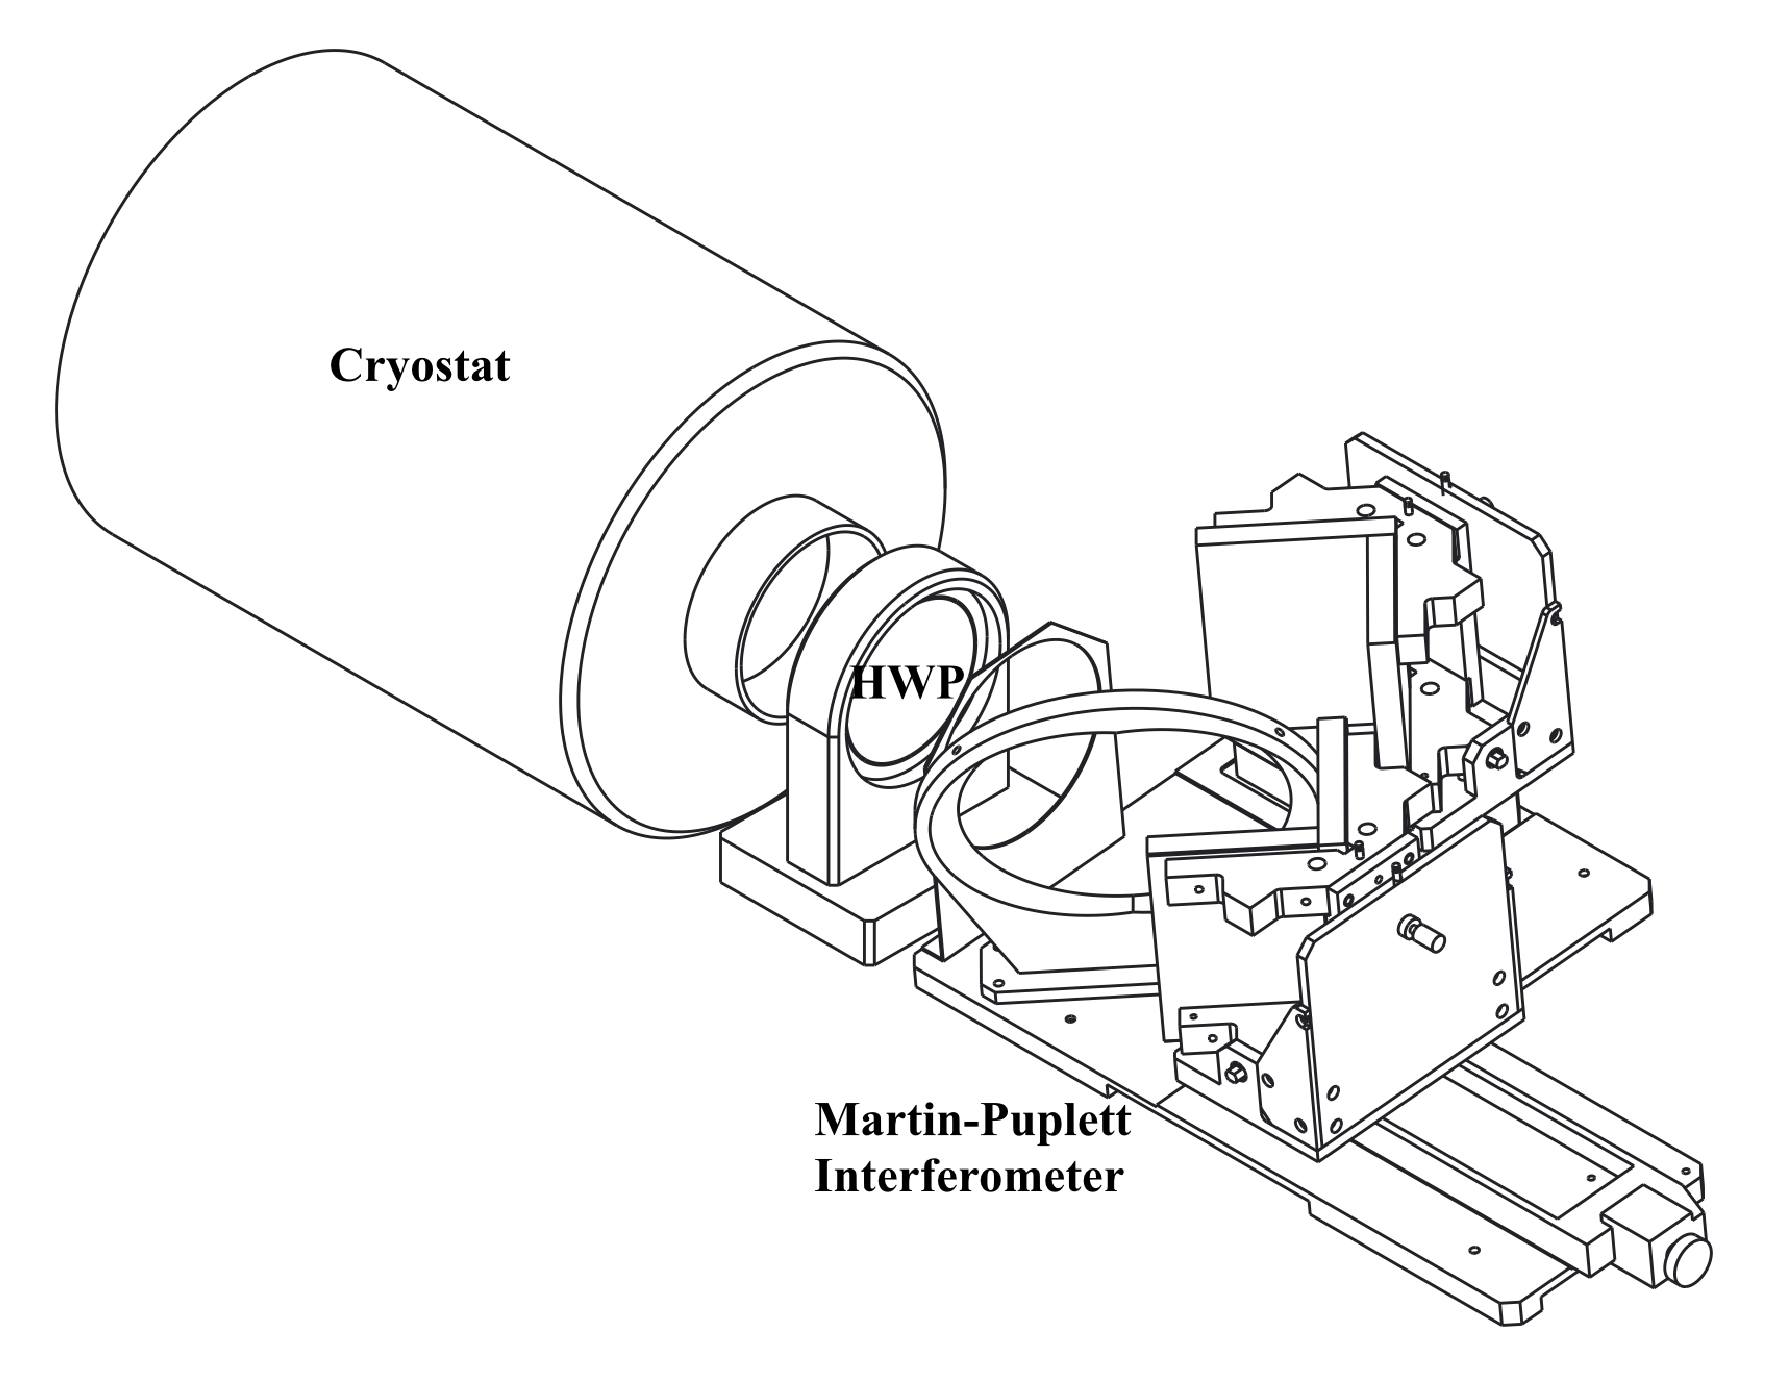
\includegraphics[width=7cm, keepaspectratio]{figures/Lab_test_config}
    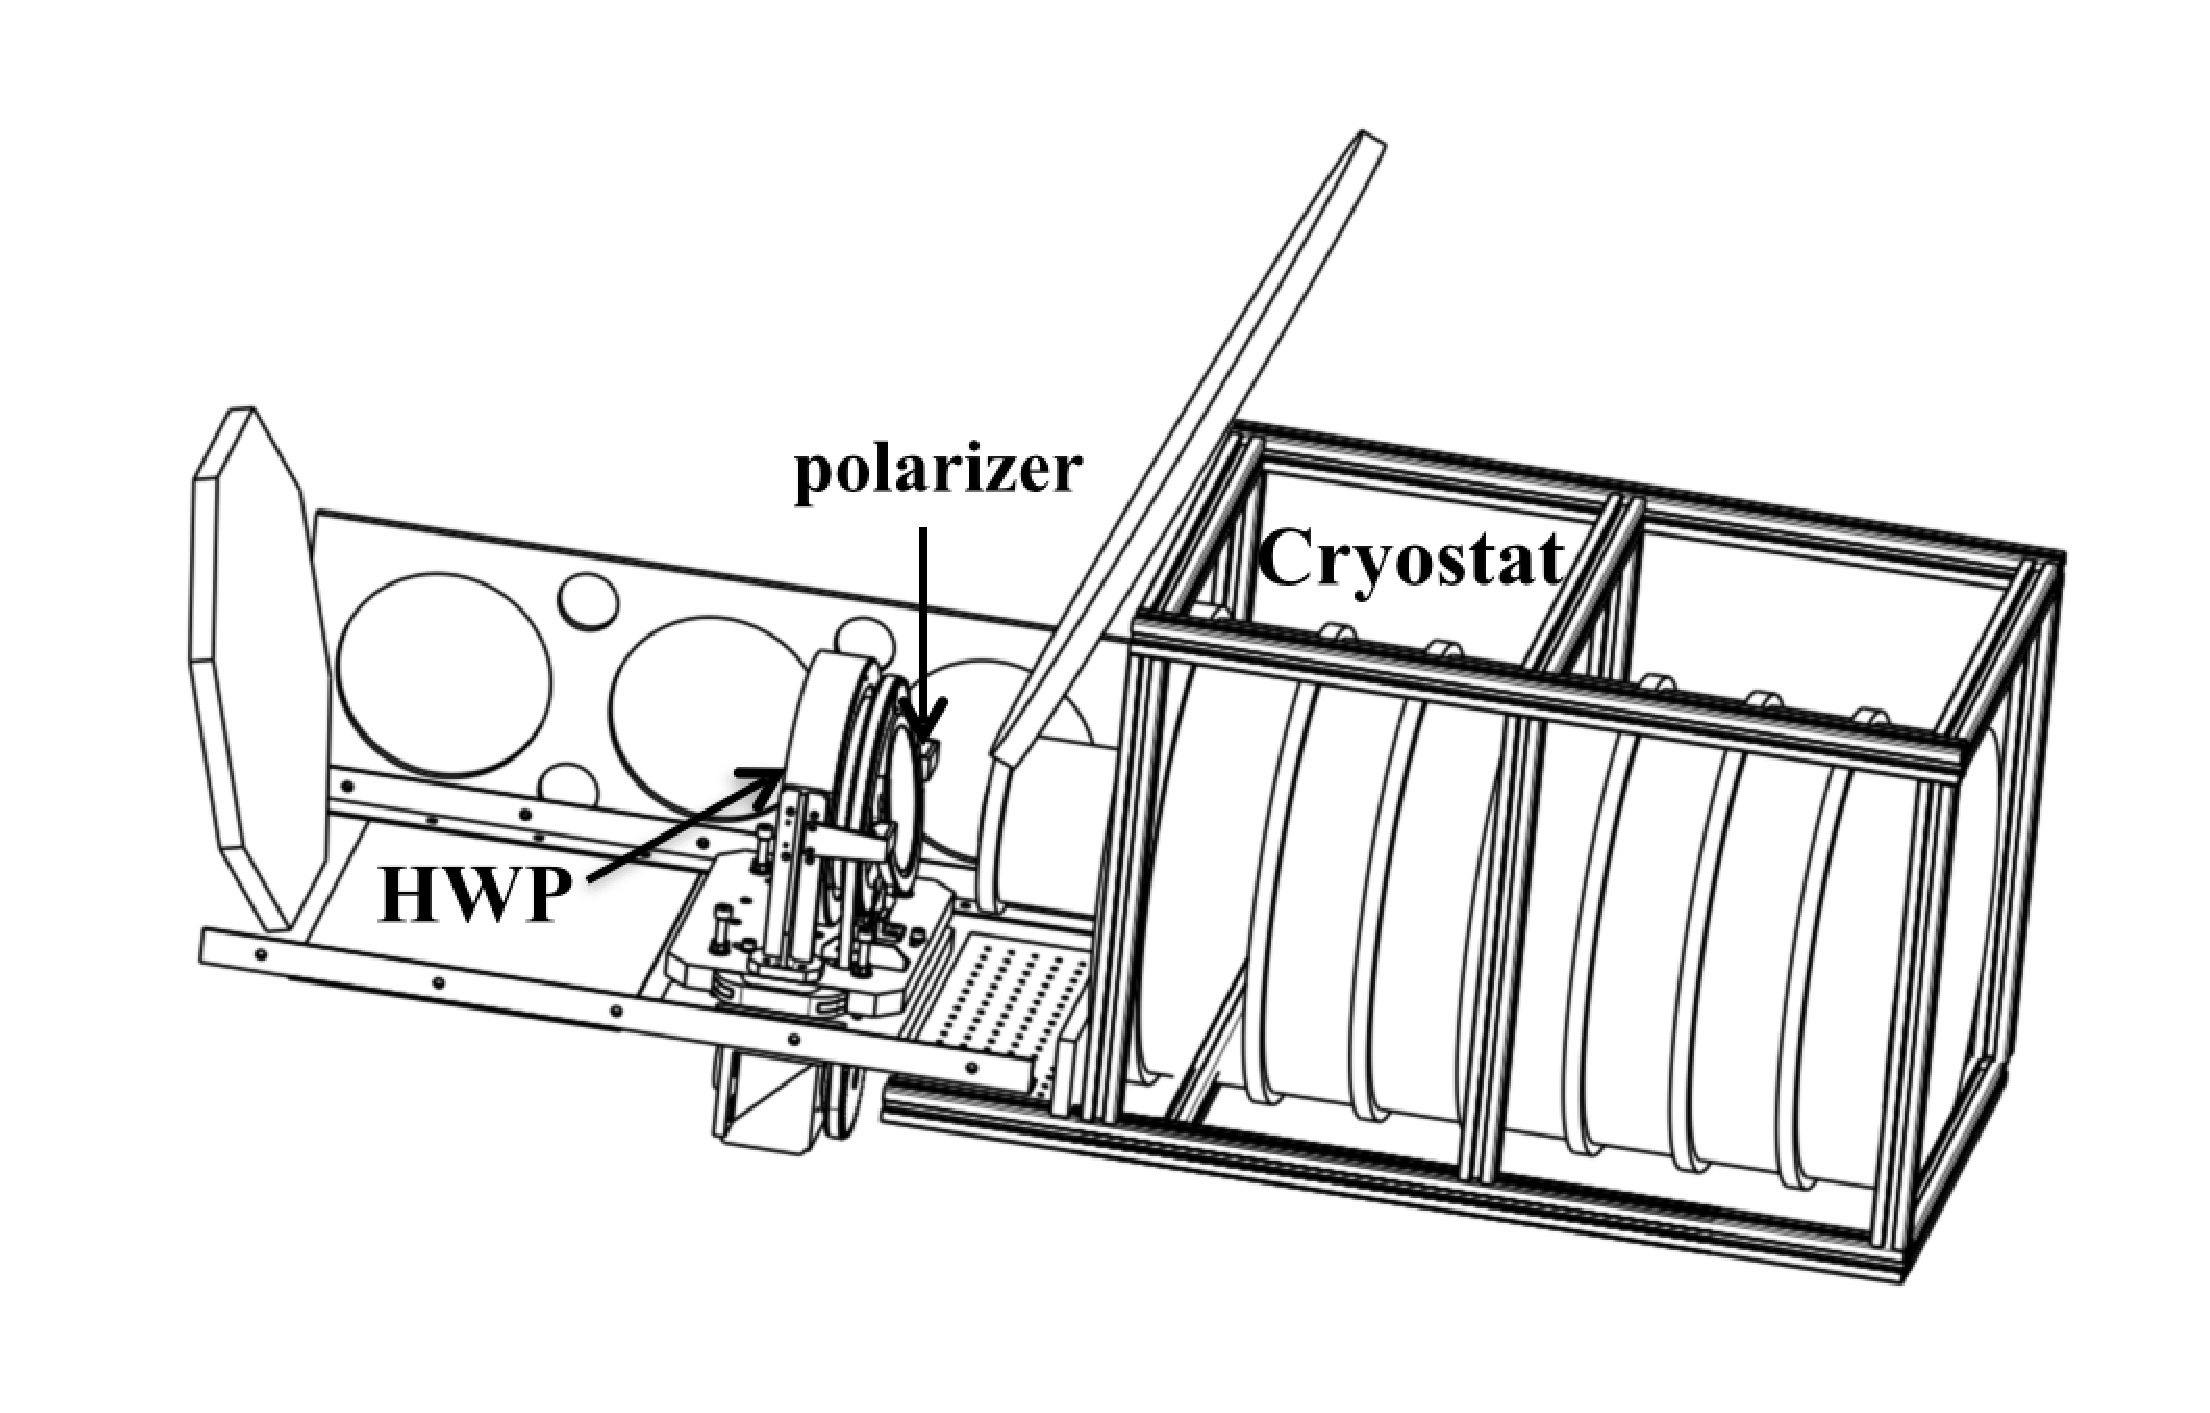
\includegraphics[width=7cm, keepaspectratio]{figures/setup_polar_telescope}
    \caption{Left: Laboratory instrumental setup {\nico:} the \nika\ cryostat,
      the HWP in a fixed position and a Martin-Puplett interferometer. Right:
      Instrumental setup for polarization measurements at the telescope {\nico
        with the last two mirrors of the optics chain and the polarization
        module with the HWP and the stepper motor mounted in front of the
        entrance window of the cryostat. The polarizer is tilted by about 10
        degrees to avoid standing waves}. \label{polarsetup}}
  \end{center}
\end{figure*}
\begin{figure}[t!]
  \begin{center}
   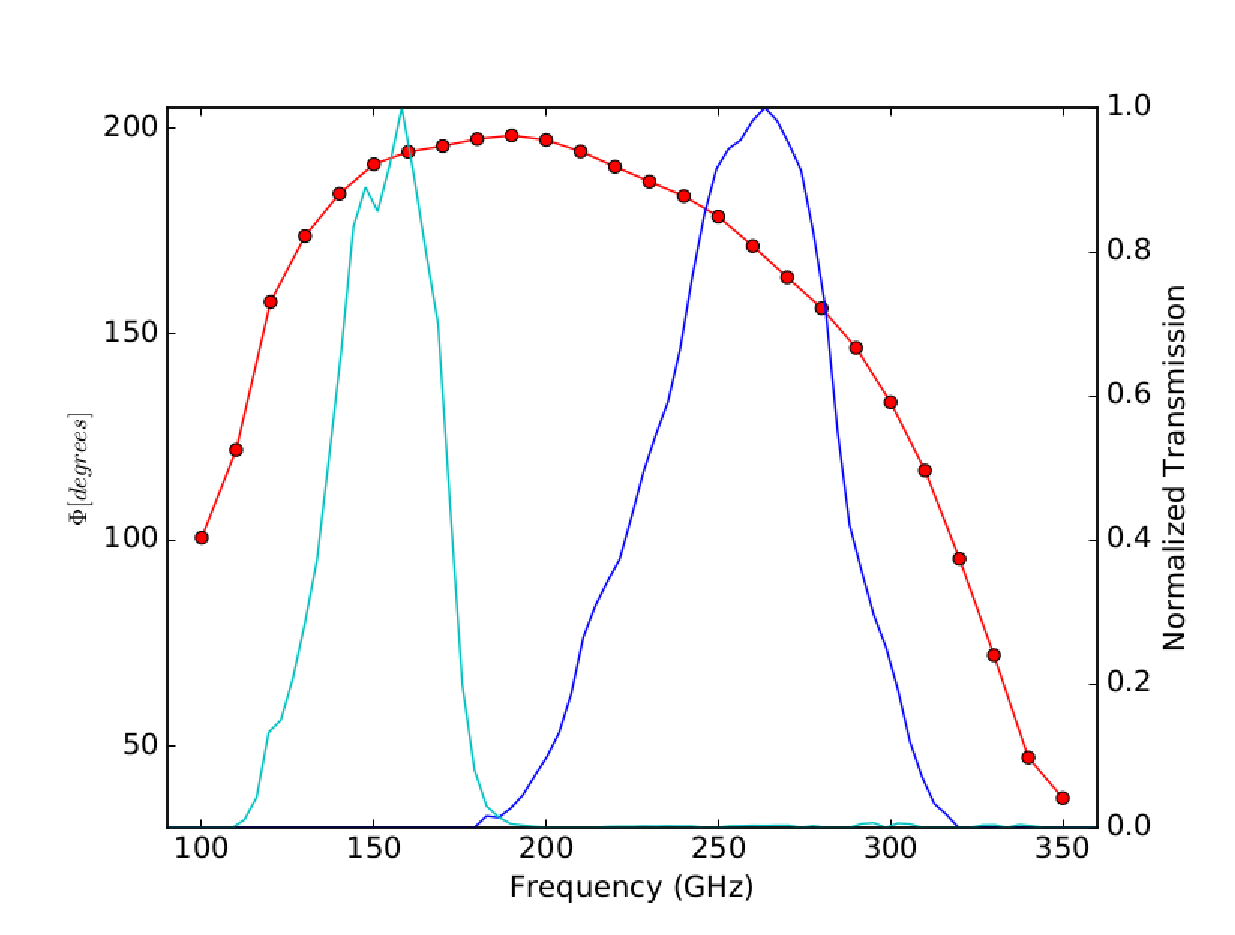
\includegraphics[width=6.5cm, keepaspectratio]{figures/phase_shift_angle}
   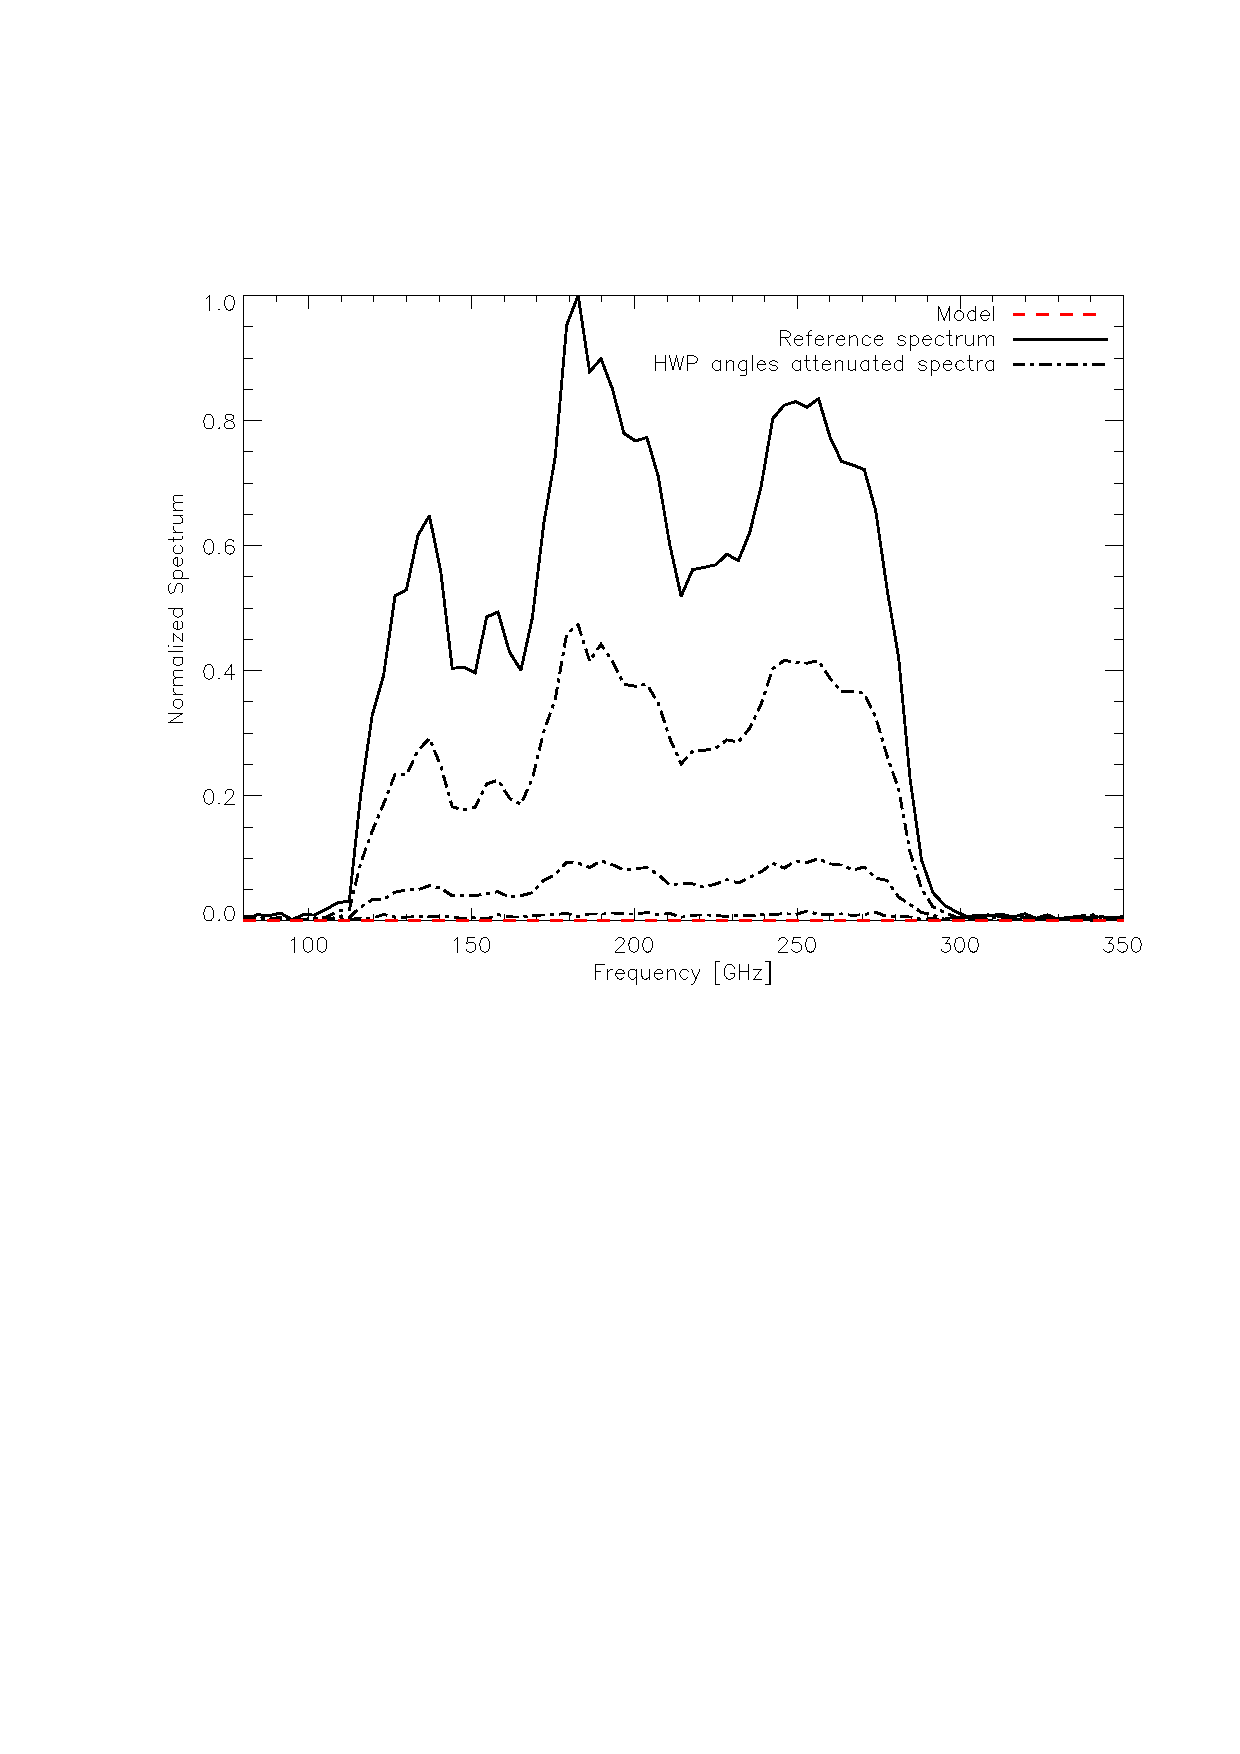
\includegraphics[width=6.5cm, keepaspectratio]{figures/spectre}
    \caption{Top: Phase shift angle as a function of frequency for the \nika\ HWP. The transmission for the two \nika\ frequency bands
    at 1 (blue) and 2 (cyan) mm are also plotted for illustration. Bottom: 
    Spectral transmission of the \nika\ HWP at different angles with respect to the optical axis.
    The red curve corresponds to the best-fit model for the intermediate angle data.}
    
%    Maximum transmission at an angle of 46.8$^{\circ}$
 %    respect to the HWP zero and attenuated spectra at 72$^{\circ}$,
%      79$^{\circ}$, 86.4$^{\circ}$ (top curve to bottom curve). For example, the
 %   model (red dotted line) fits the spectrum at an angle of 72$^{\circ}$.}
    \label{fig:spectre}
  \end{center}
\end{figure}
\begin{figure}
\includegraphics[width=1.\linewidth,keepaspectratio]{figures/toi_simu.eps}
\caption{The top panel shows the power spectrum of a simulated detector observed TOI for a polarized point source
  observed under a raster scan, and polarization modulation by a continuously
  rotating HWP facing a polarization analyser. The raw signal plus noise TOI (black) has its total intensity
  content highlighted in cyan and the polarized content in green. The polarization
  signal band is centered on the fourth HWP harmonics while the intensity signal
  band lays at lower frequencies. On the bottom plot, we present the TOI after demodulation
  (see. Sect.~\ref{se:lockin}). We observe that half of its Stokes $Q$ content has been put at
  low frequency while the Stokes $I$ content and the remaining polarized contents are
  shifted at frequencies higher than the signal band.}
   \label{fig:toi_simu}
\end{figure}  
%\section{Observation strategy for polarization measurements}
\begin{figure*}
  \begin{center}
  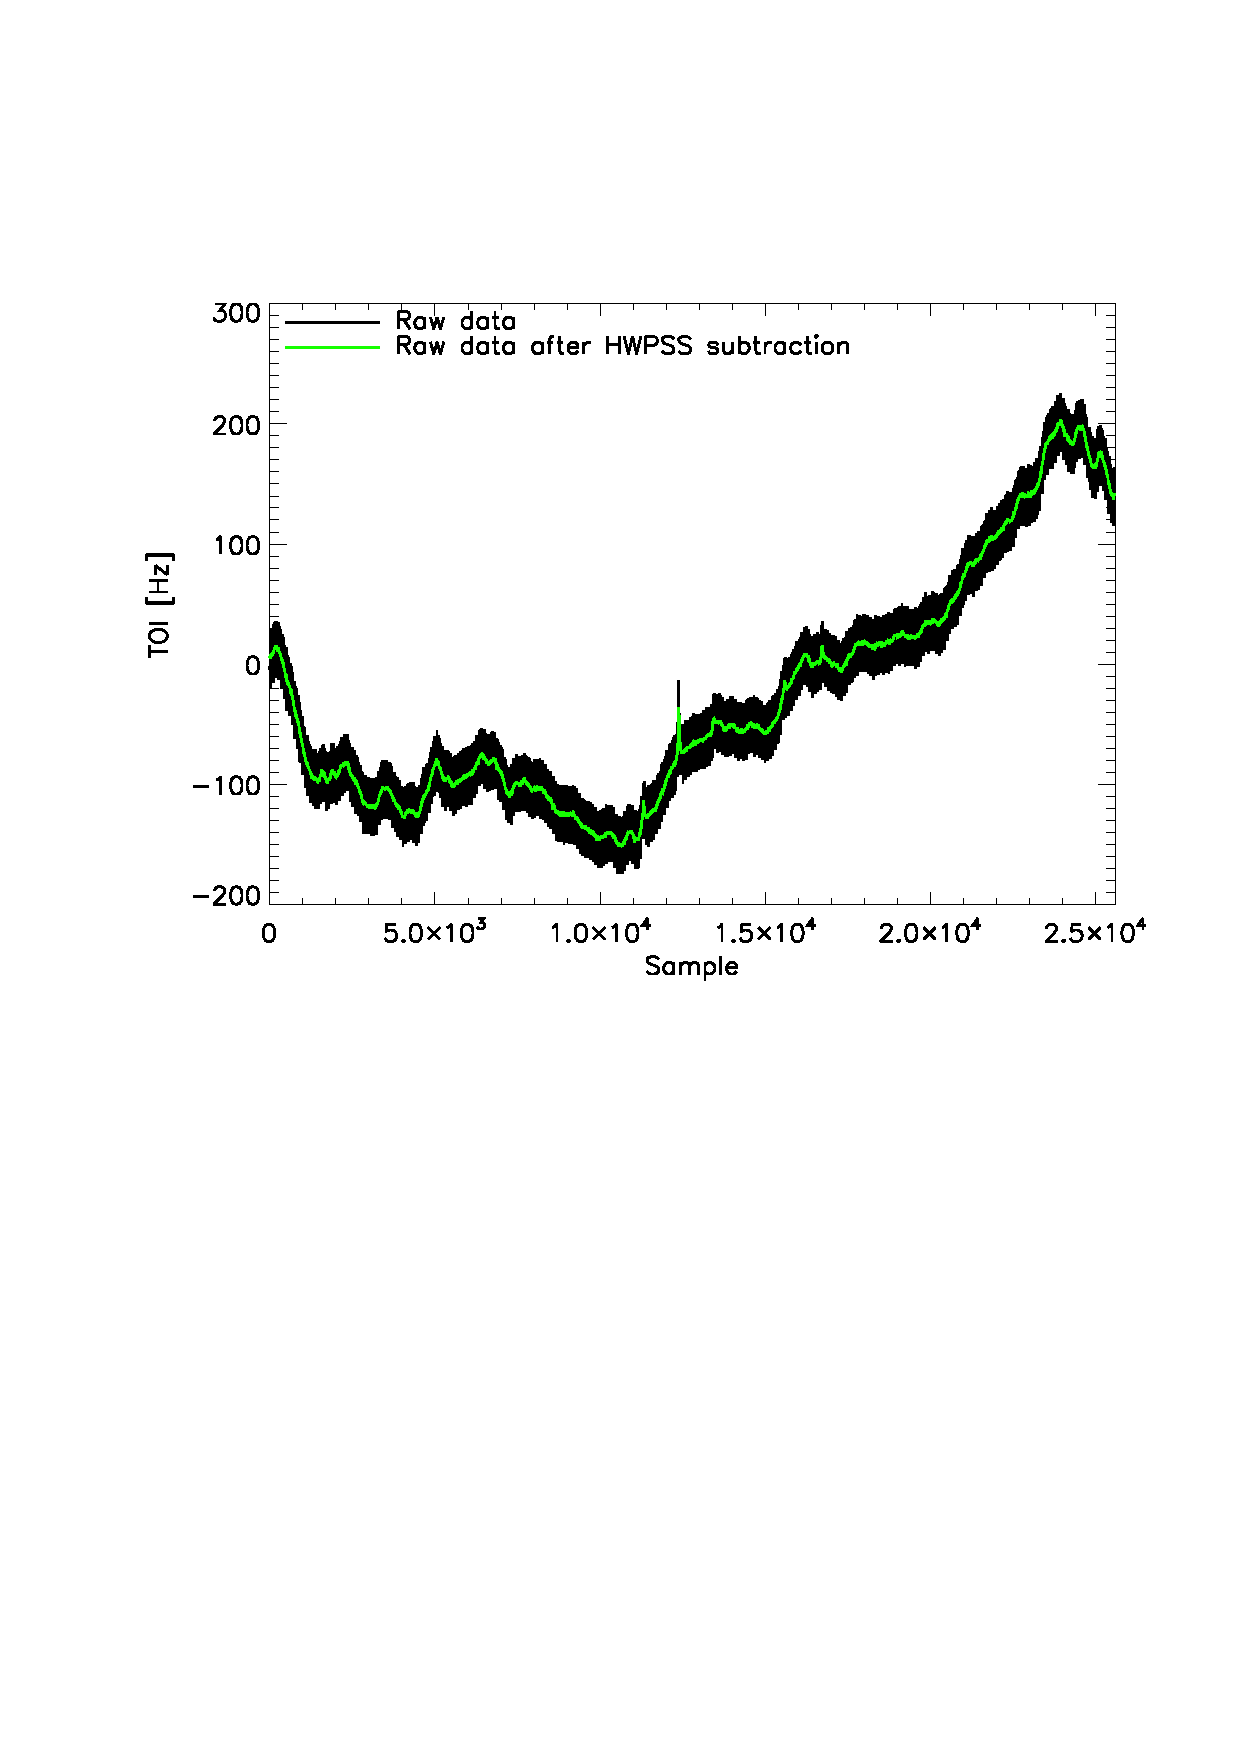
\includegraphics[%
  width=8cm, keepaspectratio]{figures/TOI}
  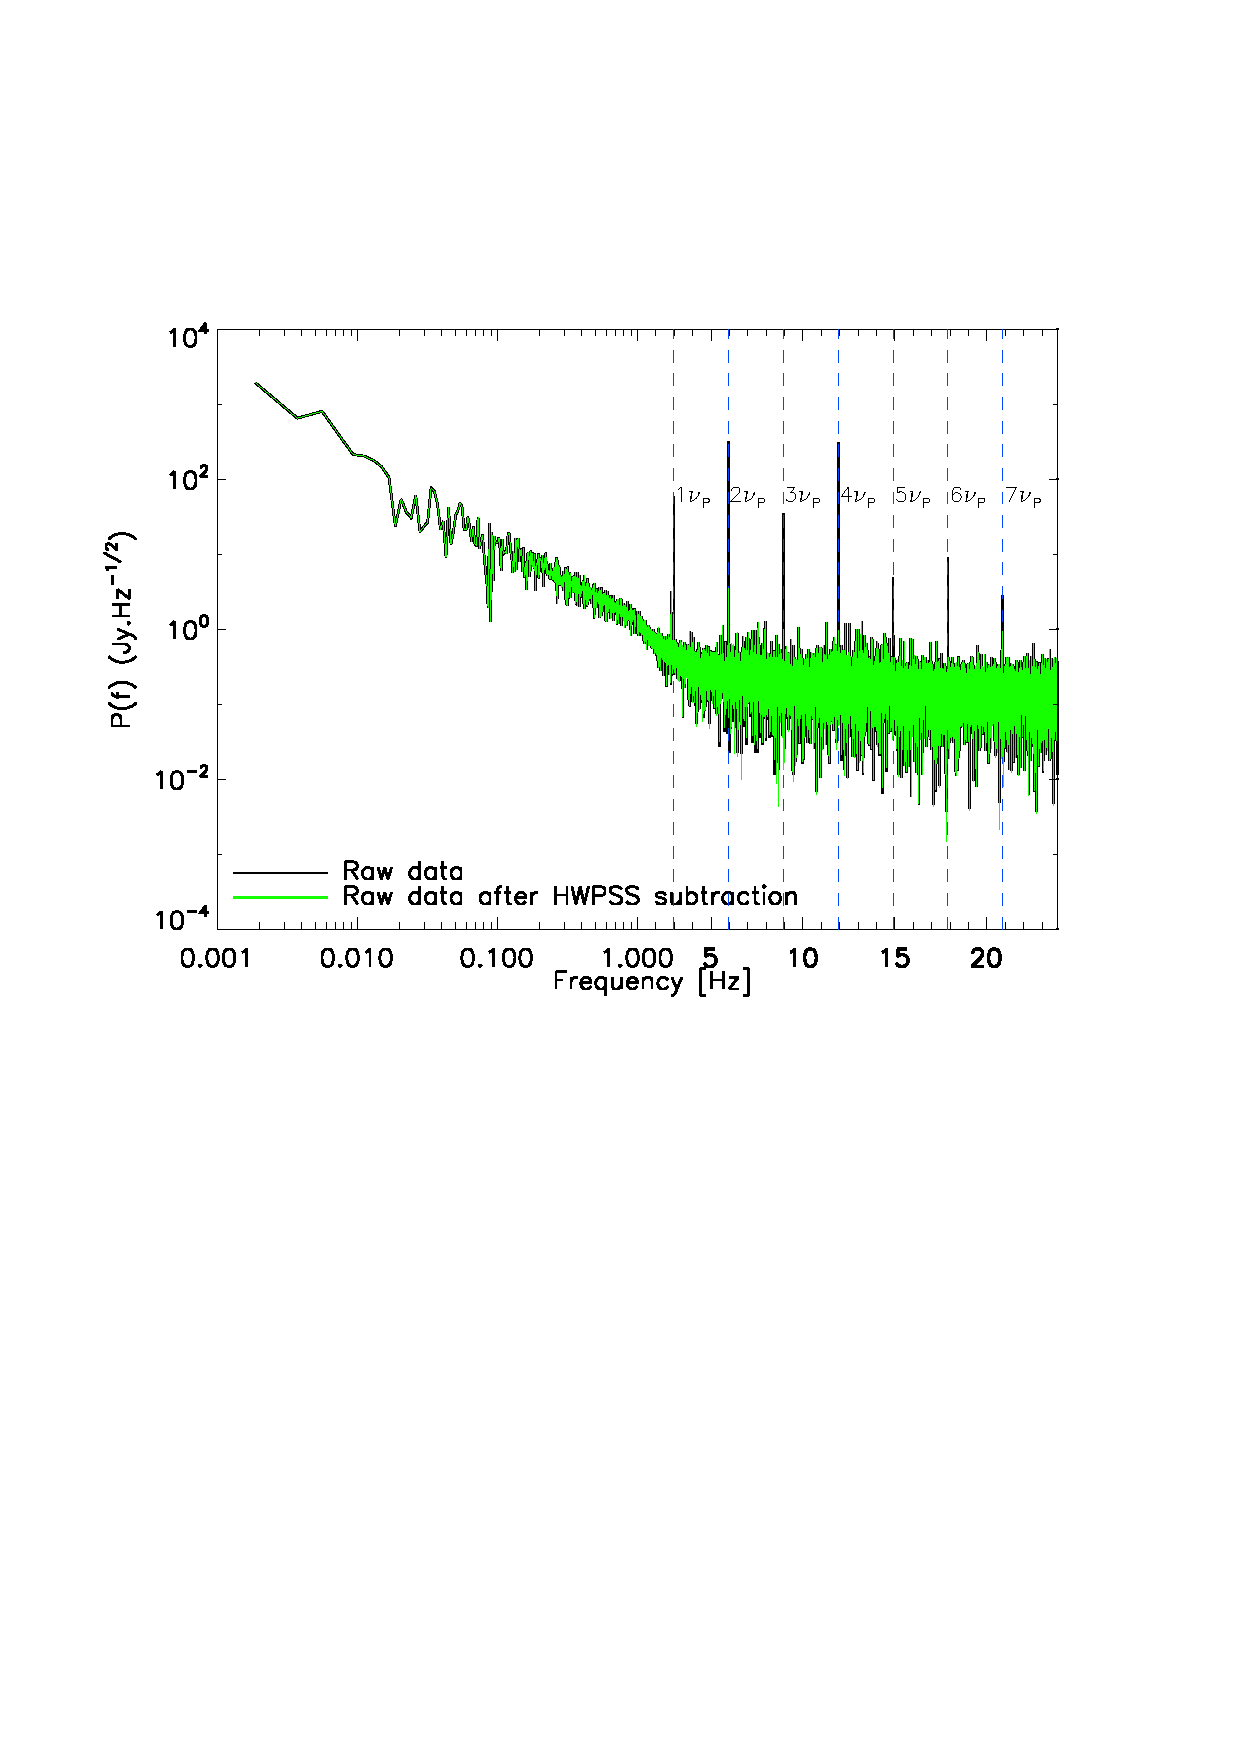
\includegraphics[%
  width=7.5cm, keepaspectratio]{figures/spectre_I_fit}
\caption{TOI (left) and power spectrum (right) of an observation of Orion OMC-1
  for a single KID. Raw data are presented in black and the HWPSS subtracted
  data in green.{\nico refaire le plot du power spec en log/lin, facile.}}
  \label{toi_i}
   \end{center}
   \end{figure*}  
 \begin{figure*}
   \begin{center}
     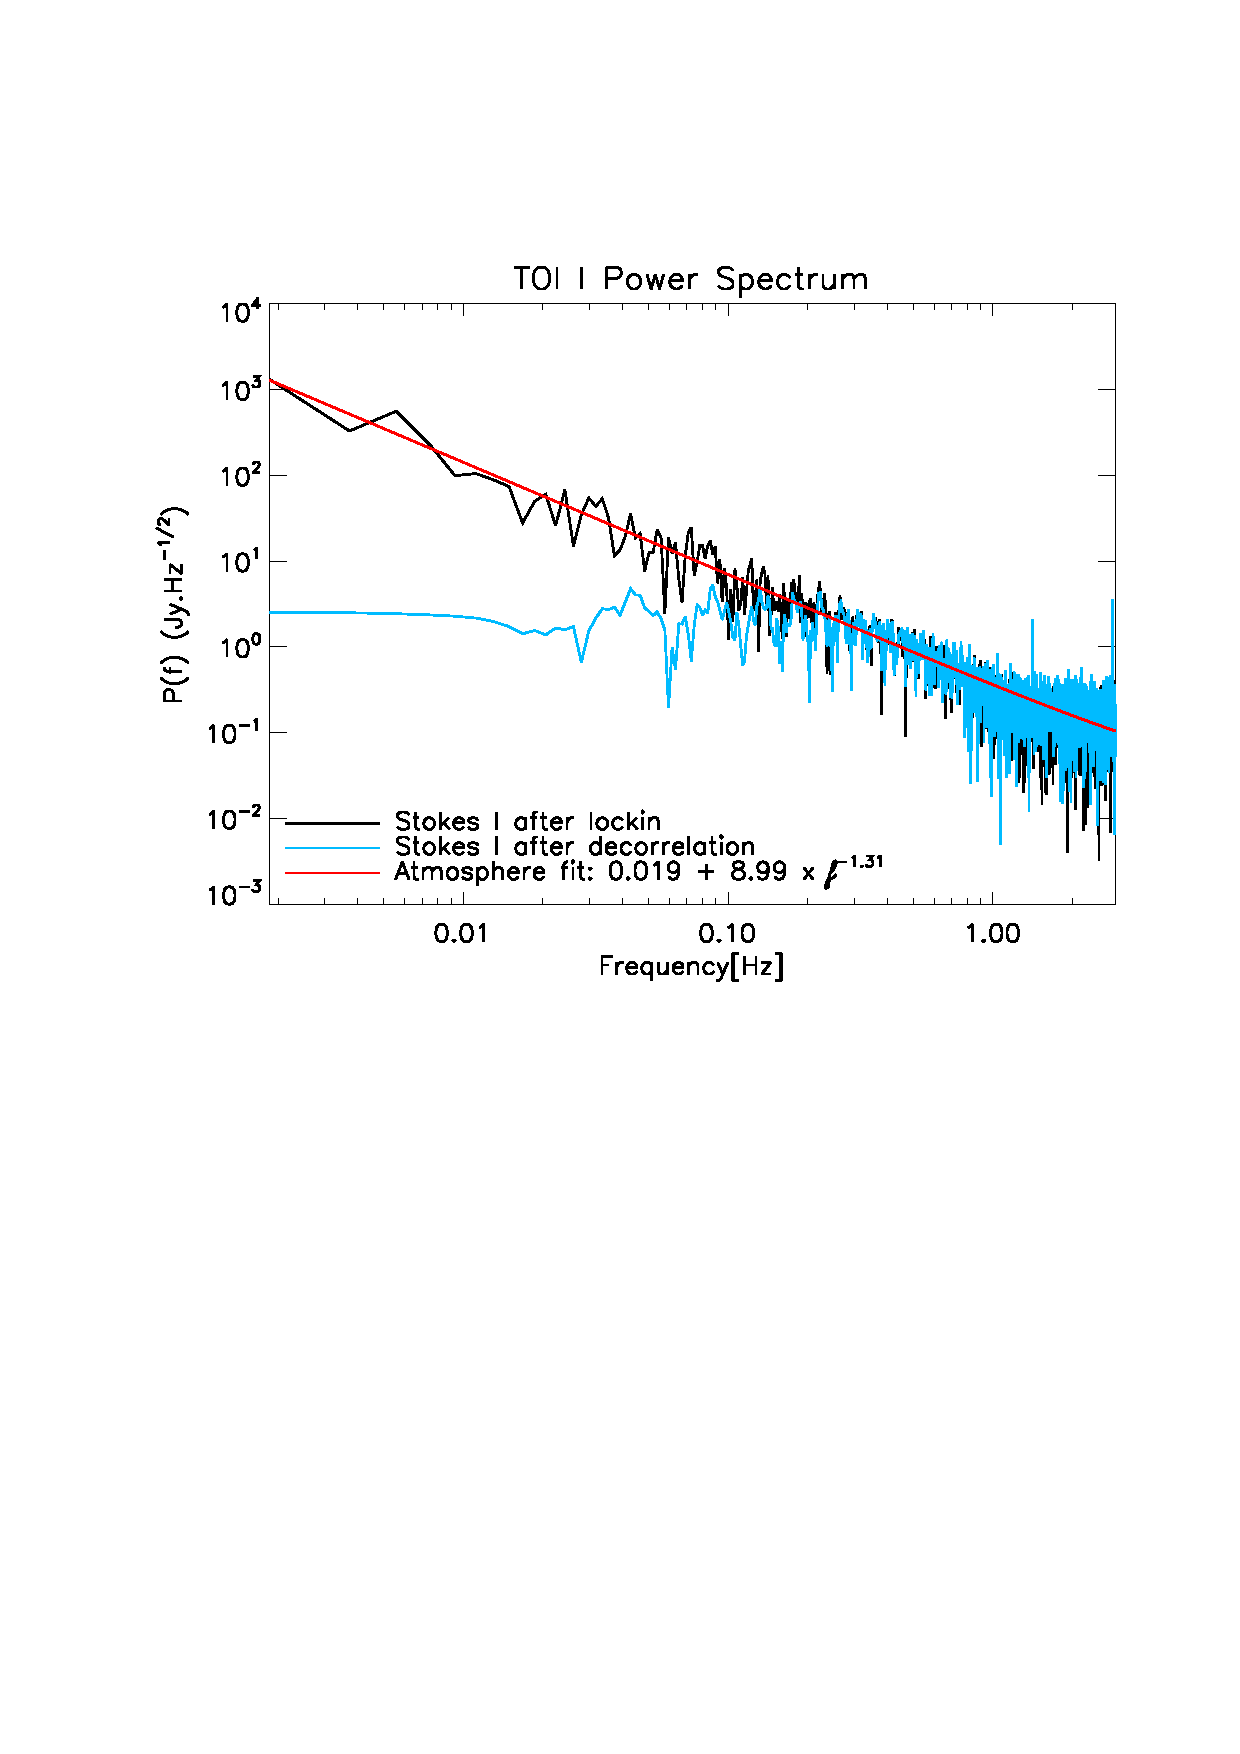
\includegraphics[%
       width=5.8cm,keepaspectratio]{figures/spectre_I_fit_decor}
     \includegraphics[%	
       width=6cm,keepaspectratio]{figures/spectre_Q_fit}
     \includegraphics[%	
       width=6cm,keepaspectratio]{figures/spectre_U_fit}
     \caption{From left to right power spectra of the Stokes $I$, $Q$, $U$ pure
       TOIs (black) after applying the lock-in procedure to the raw data in
       Figure~\ref{toi_i}.  A bandpass filter is applied to reject any high
       frequency noise. In blue we also show the power spectra after applying
       the decorrelation procedure to the demodulated data.  See
       Section~\ref{se:demod_mapmaking} for details.{\nico I'd rather show the
         power spectra after hwpss subtraction and lockin here to illustrate our
       speech more specifically, and avoid questions about the noise boost above
       fcut during decorrelation.}}
     \label{spectre_iqu}
   \end{center}
 \end{figure*}

\begin{figure}
  \begin{center}
    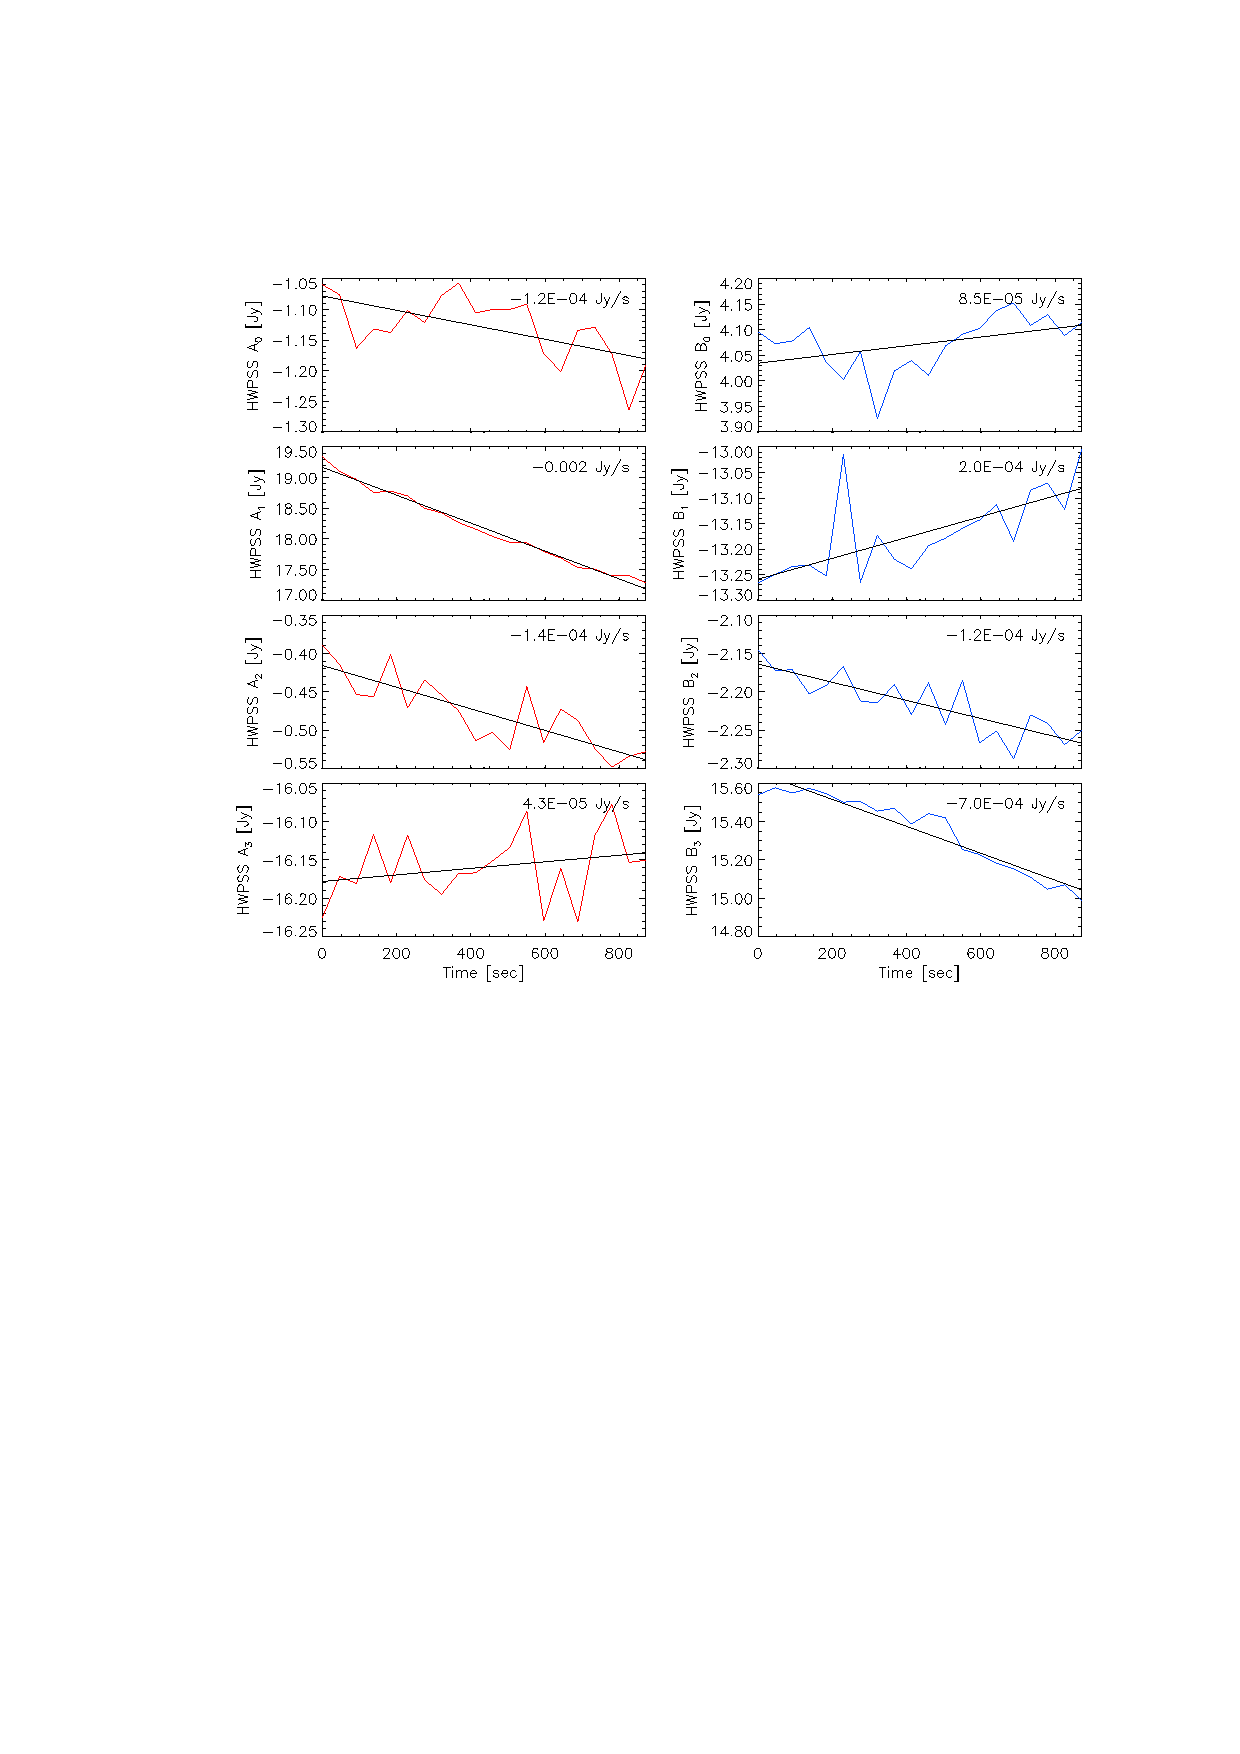
\includegraphics[%
      width=1.\linewidth,keepaspectratio]{figures/template_drift.pdf}
    \caption{\nico Percentage variation per second of the first four amplitudes of the HWP
        parasitic synchronous signal as modelled by eq.~\ref{eq:hwpss}, as
        monitored during a scan of 3C286. {\color{green}Je suis assez curieux du
        point bleu \`a nettement plus de 5 sigma... \`a mon avis il s'est passe un
        truc bizarre sur ce point et on ferait mieux de le virer du plot... ?}}
    \label{time_drift}
  \end{center}
\end{figure}

\begin{figure*}
  \begin{center}
\setlength{\unitlength}{\columnwidth} 
\begin{picture}(2,2.5)
%Uncorrected 1 mm
    \put(0.05,2.48){(a) 1 mm raw (top row) and leakage corrected (bottom row) Stokes $I$,$Q$ and $U$ maps}
     \put(0,1.85){ \includegraphics[width=0.33\linewidth,keepaspectratio]{figures/Uranus_I_map.pdf}}
     \put(0.7,1.85){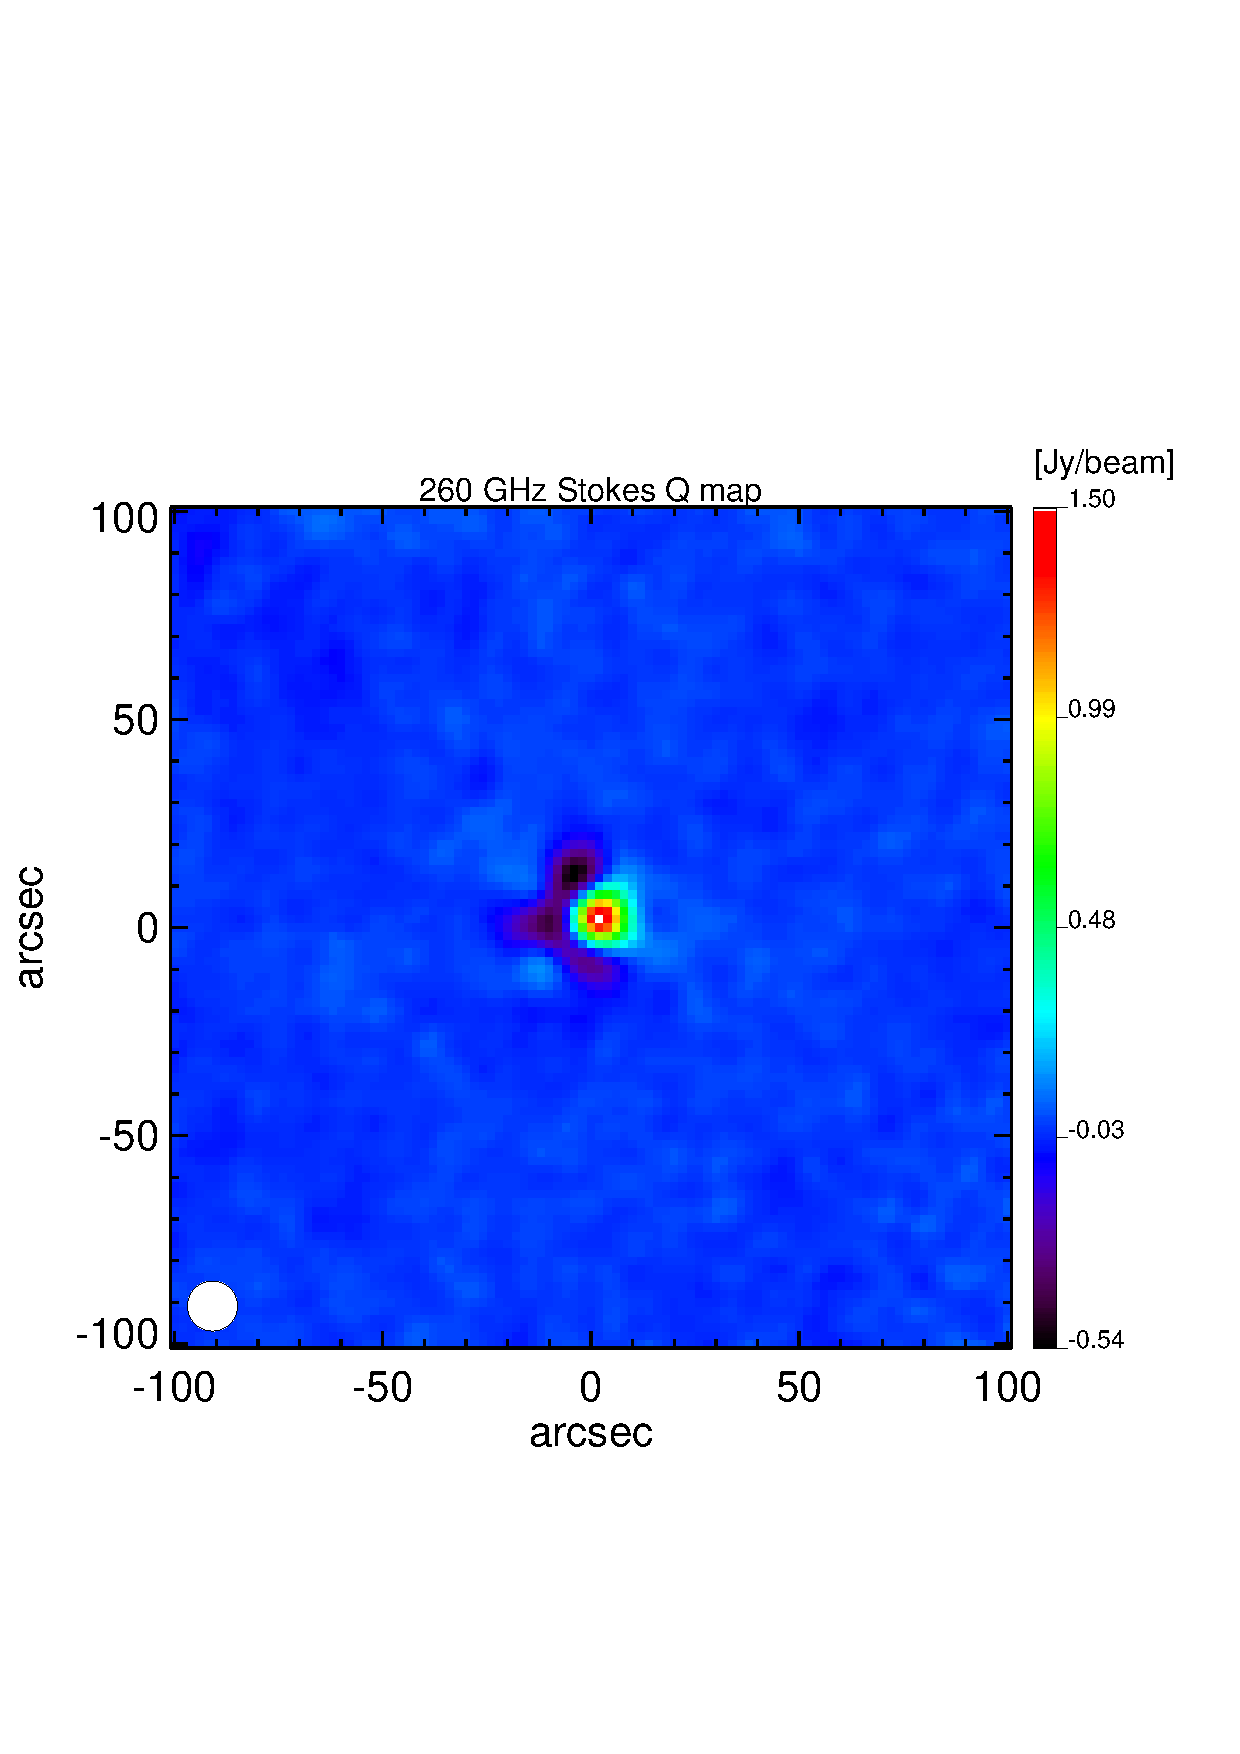
\includegraphics[width=0.33\linewidth,keepaspectratio]{figures/Uranus_Q_map.pdf}}
       \put(1.4,1.85){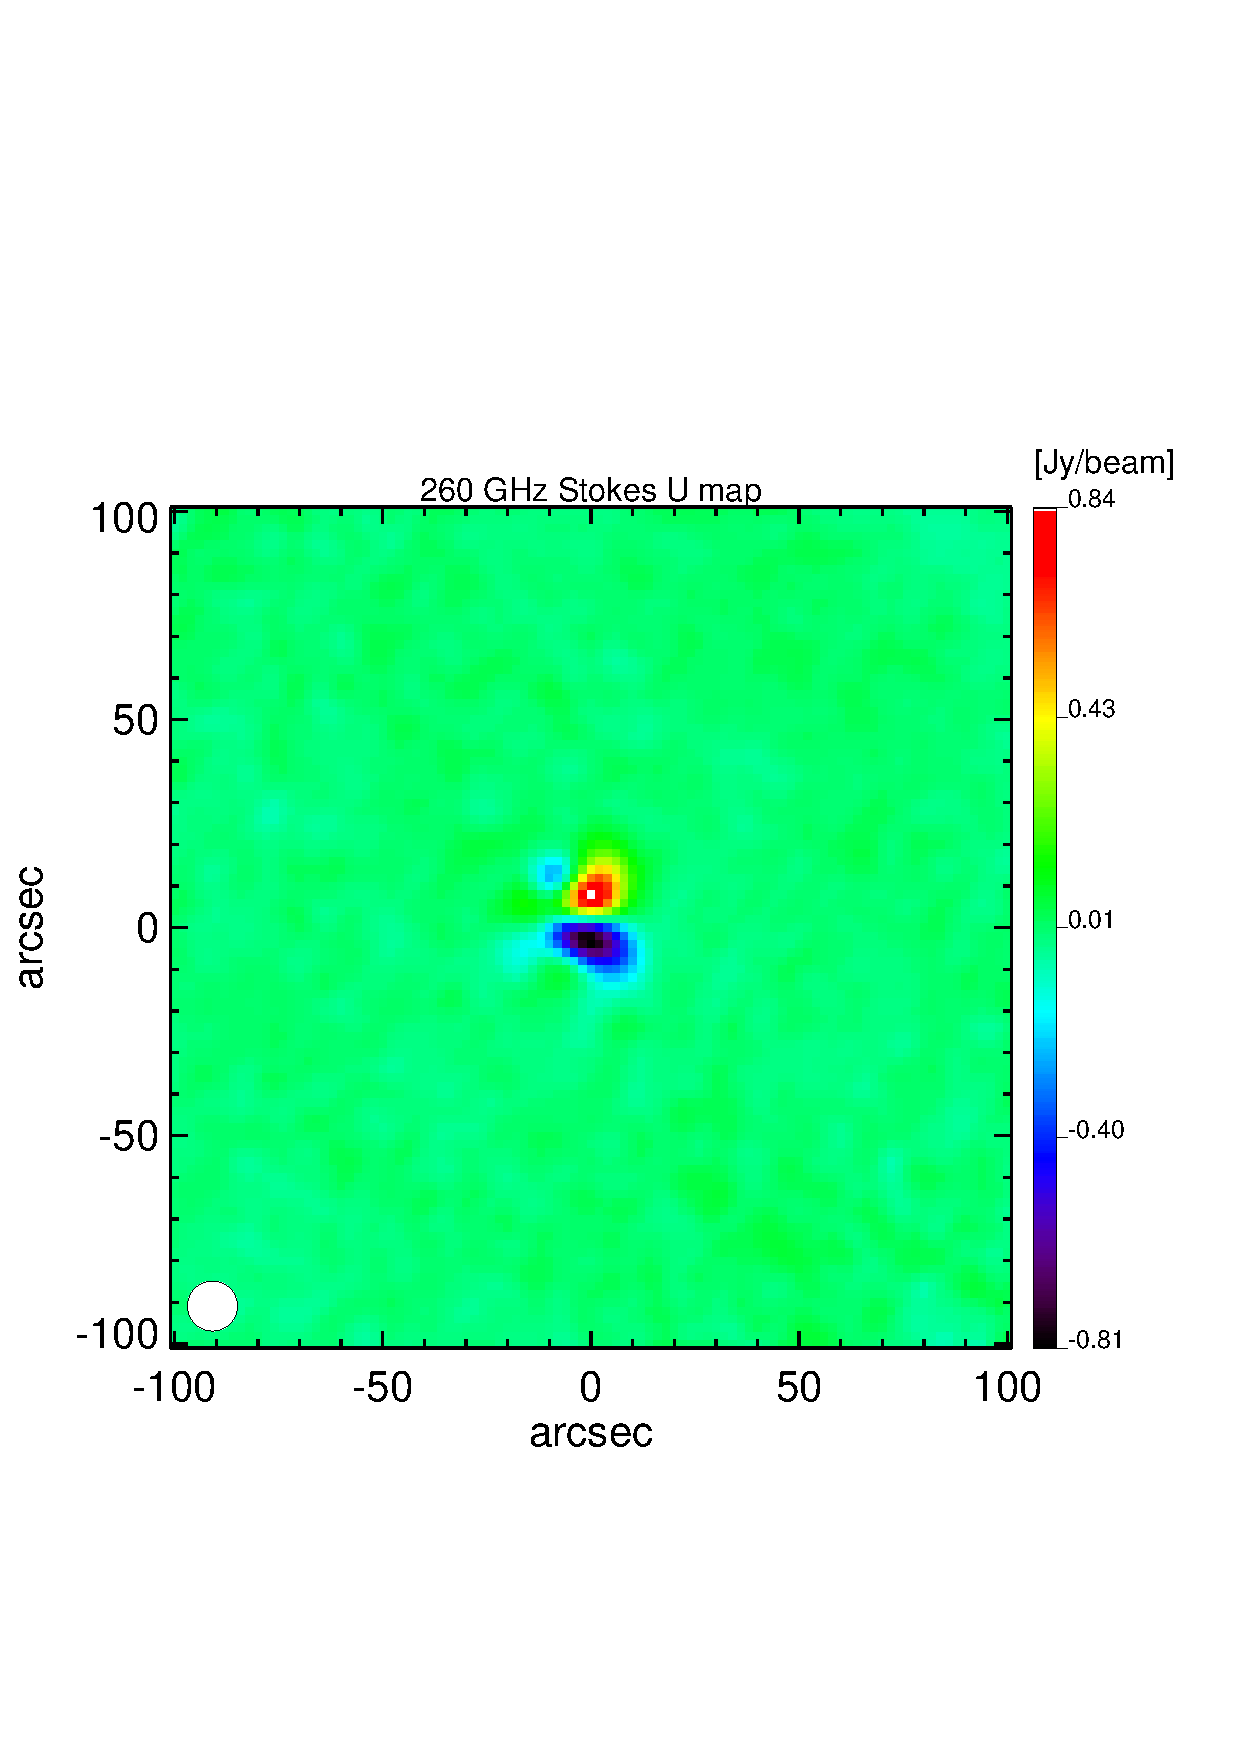
\includegraphics[width=0.33\linewidth,keepaspectratio]{figures/Uranus_U_map.pdf}}
 
 %Corrected 1 mm
     
      \put(0,1.25){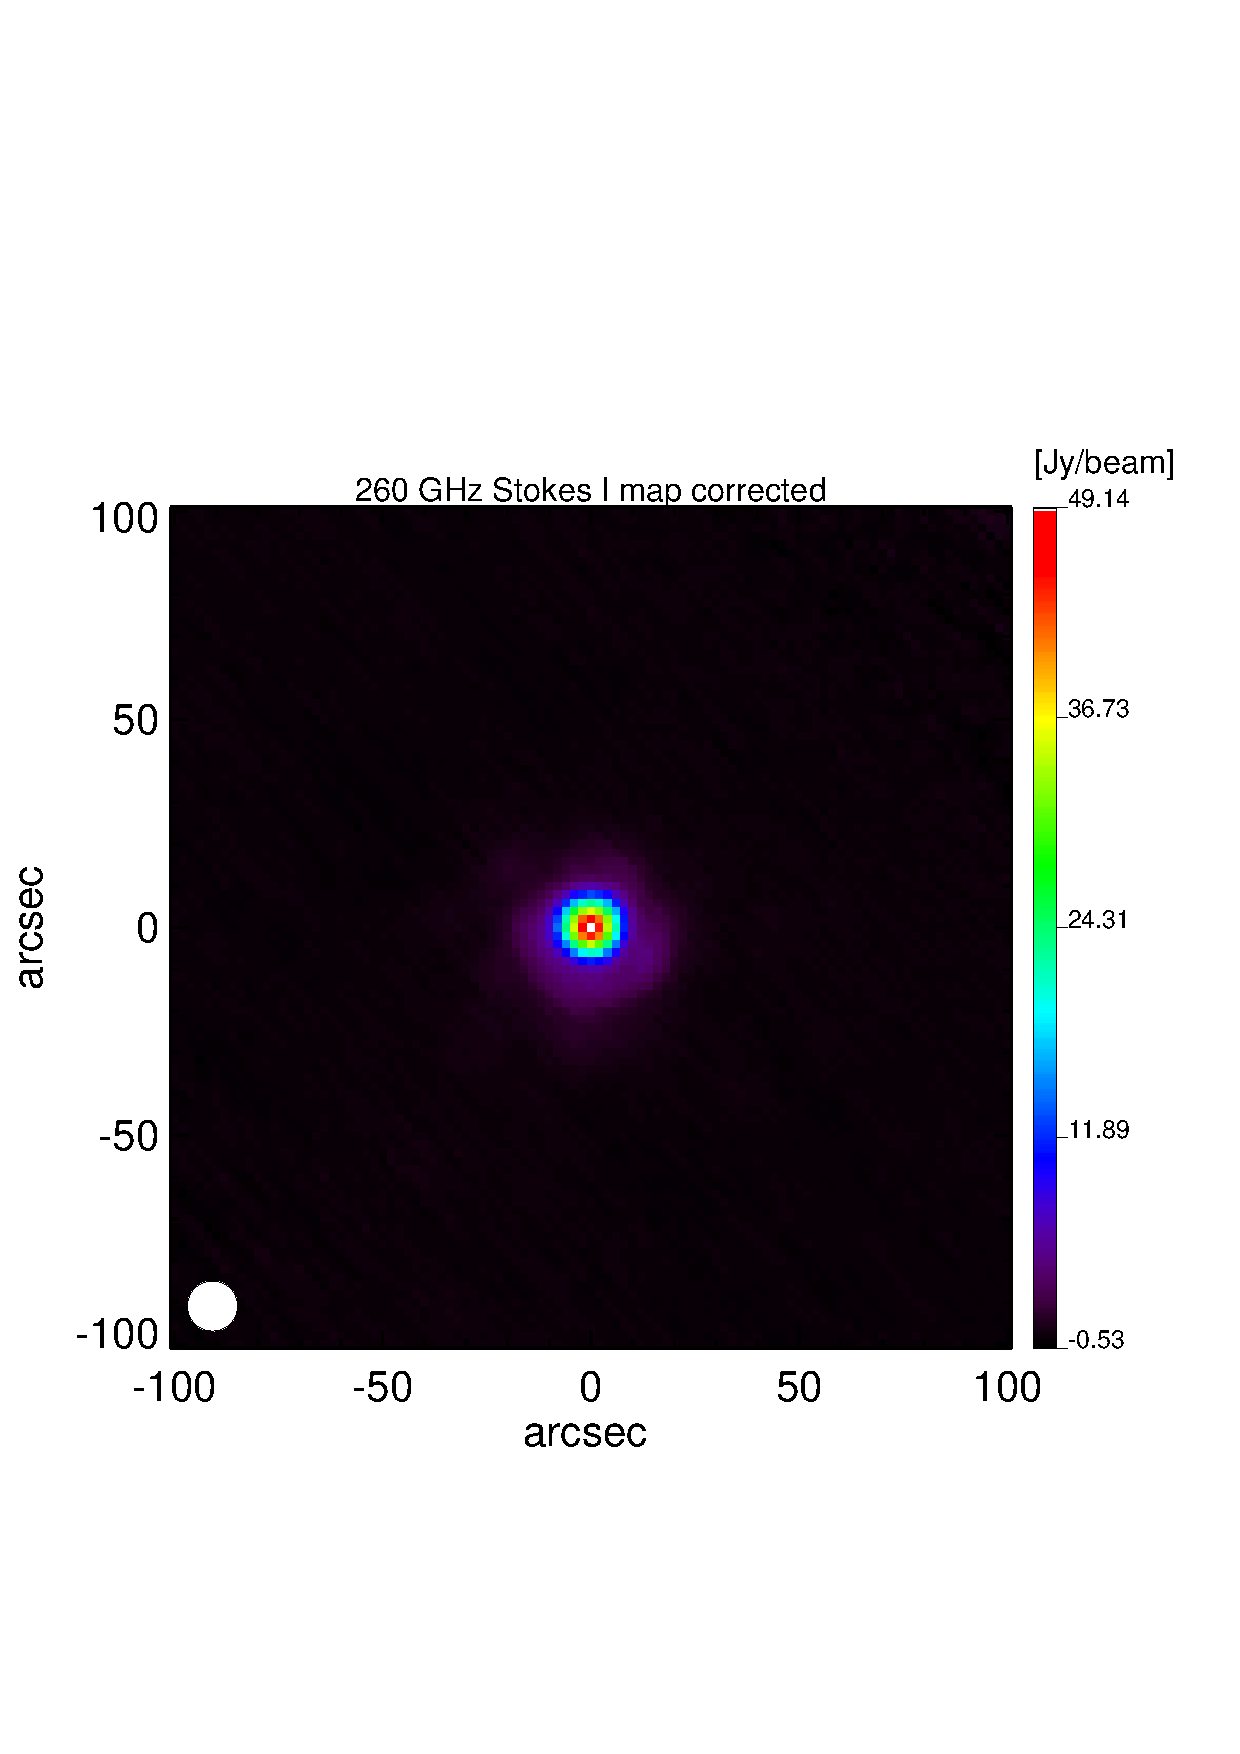
\includegraphics[width=0.33\linewidth,keepaspectratio]{figures/Uranus_I_map_corr.pdf}}
     \put(0.7,1.25){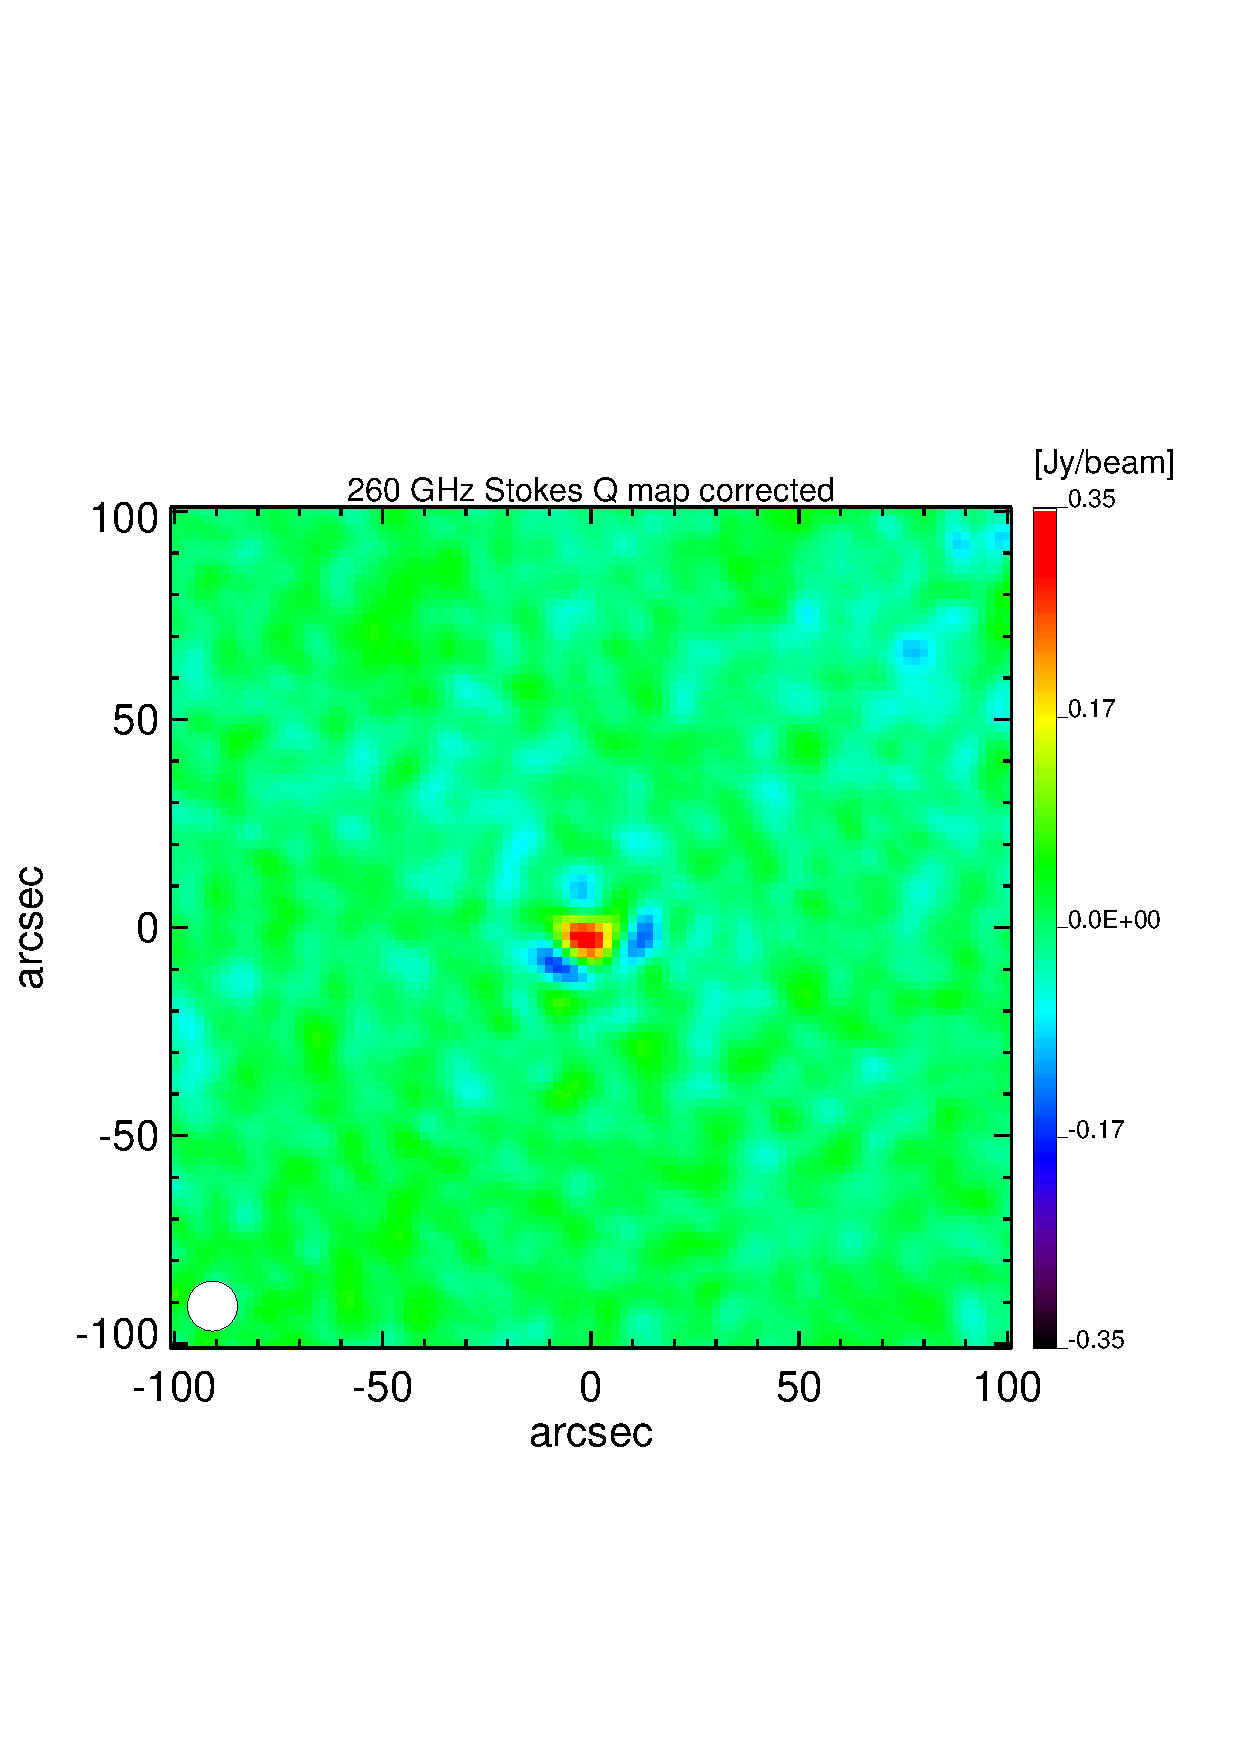
\includegraphics[width=0.33\linewidth,keepaspectratio]{figures/Uranus_Q_map_corr.pdf}}
     \put(1.4,1.25){ 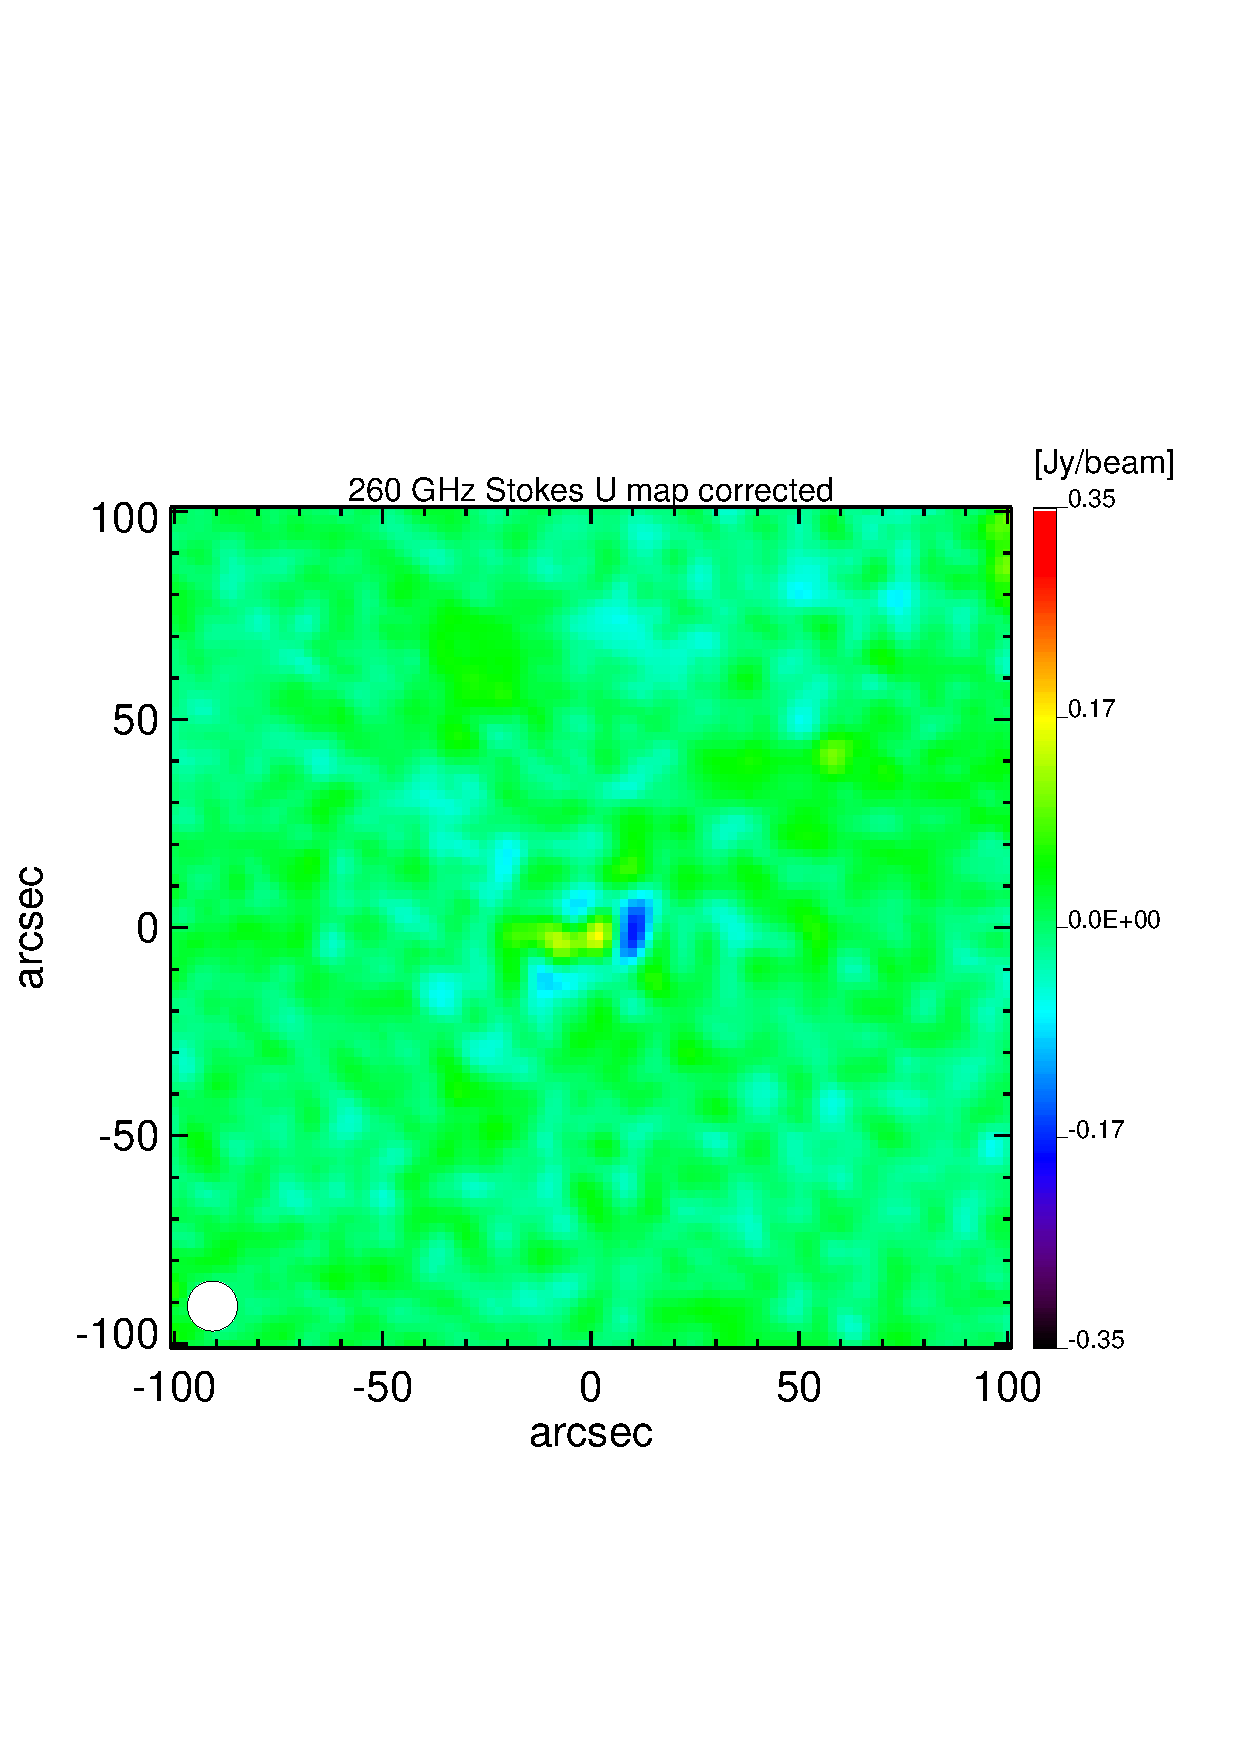
\includegraphics[width=0.33\linewidth,keepaspectratio]{figures/Uranus_U_map_corr.pdf}}

%Uncorrected 2 mm
  
    \put(0.05,1.2){(b) 2 mm raw (top row) and leakage corrected (bottom row) Stokes $I$,$Q$ and $U$ maps}

      \put(0,0.6){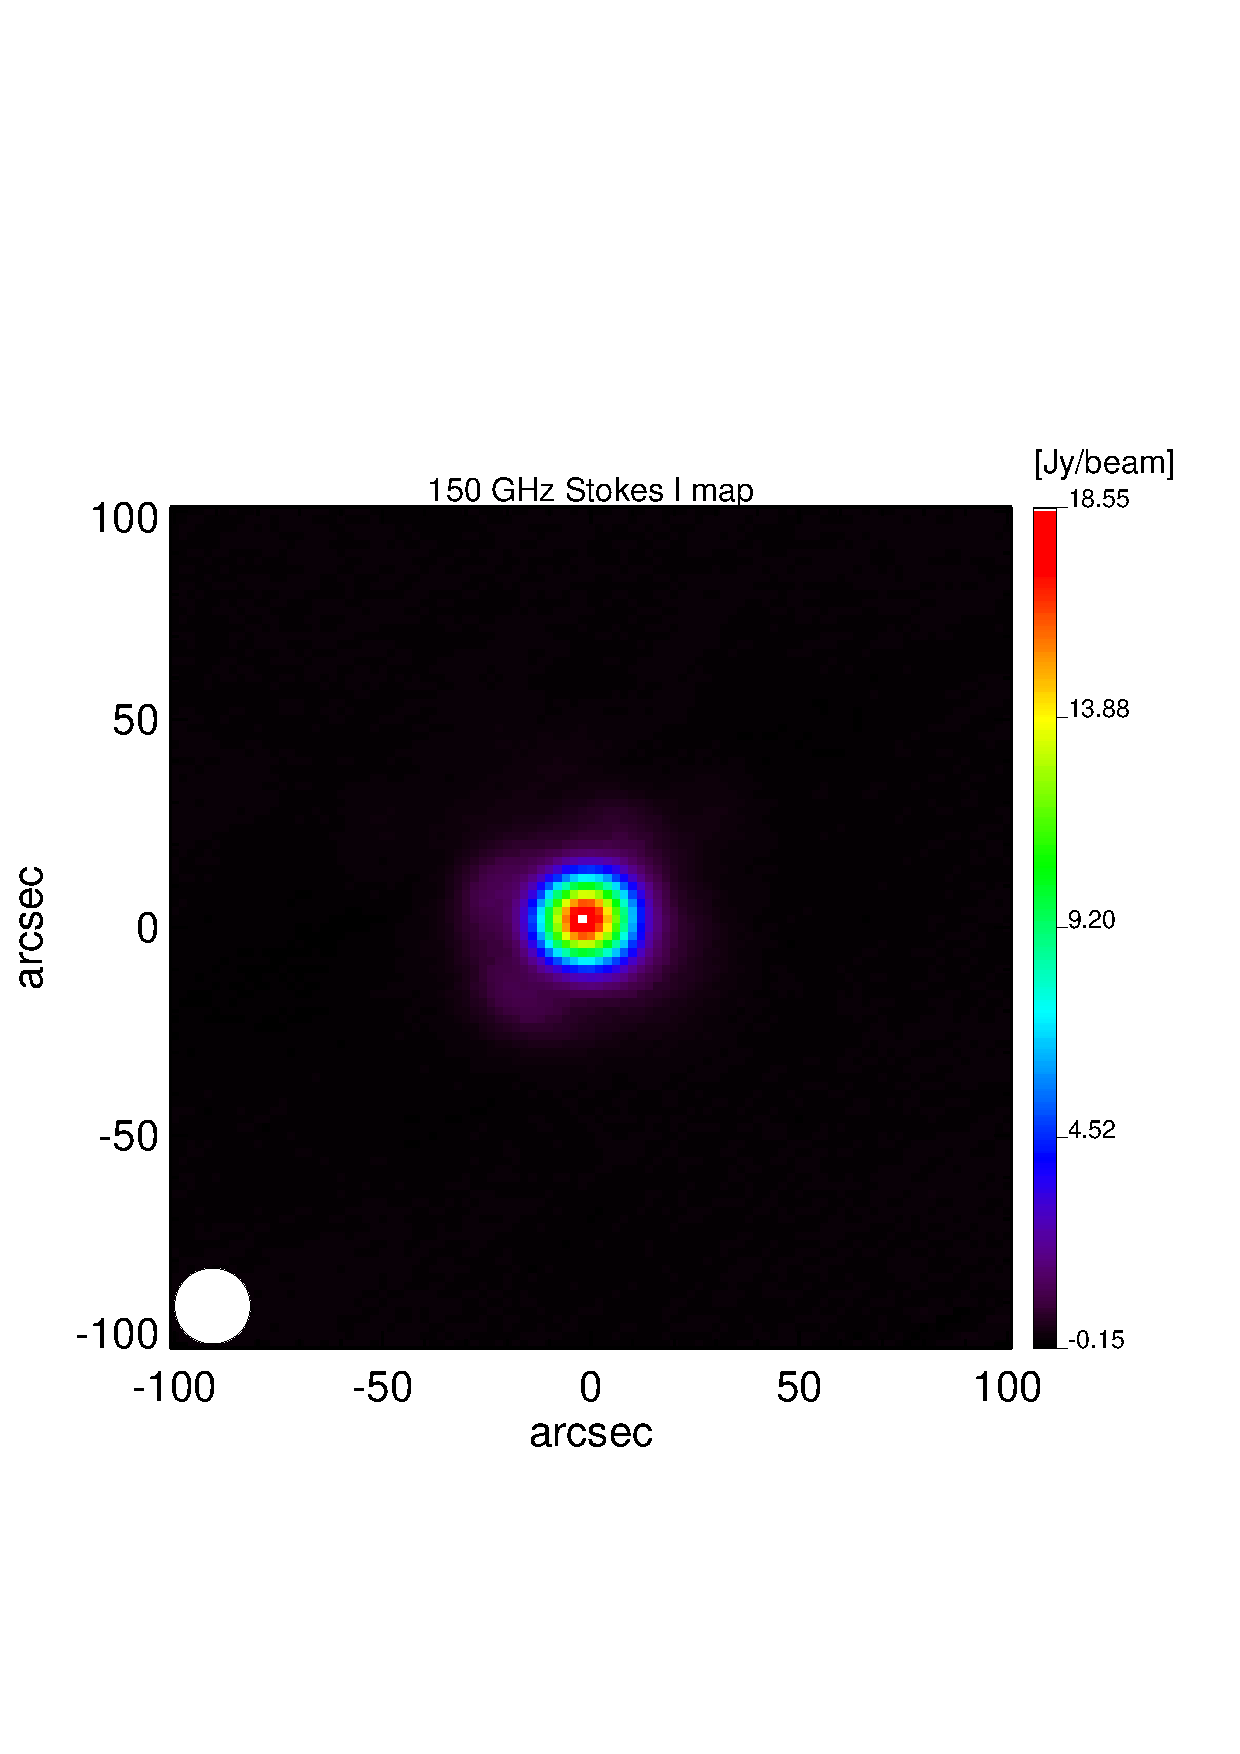
\includegraphics[width=0.33\linewidth,keepaspectratio]{figures/Uranus_I_map_2mm.pdf}}
      \put(0.7,0.6){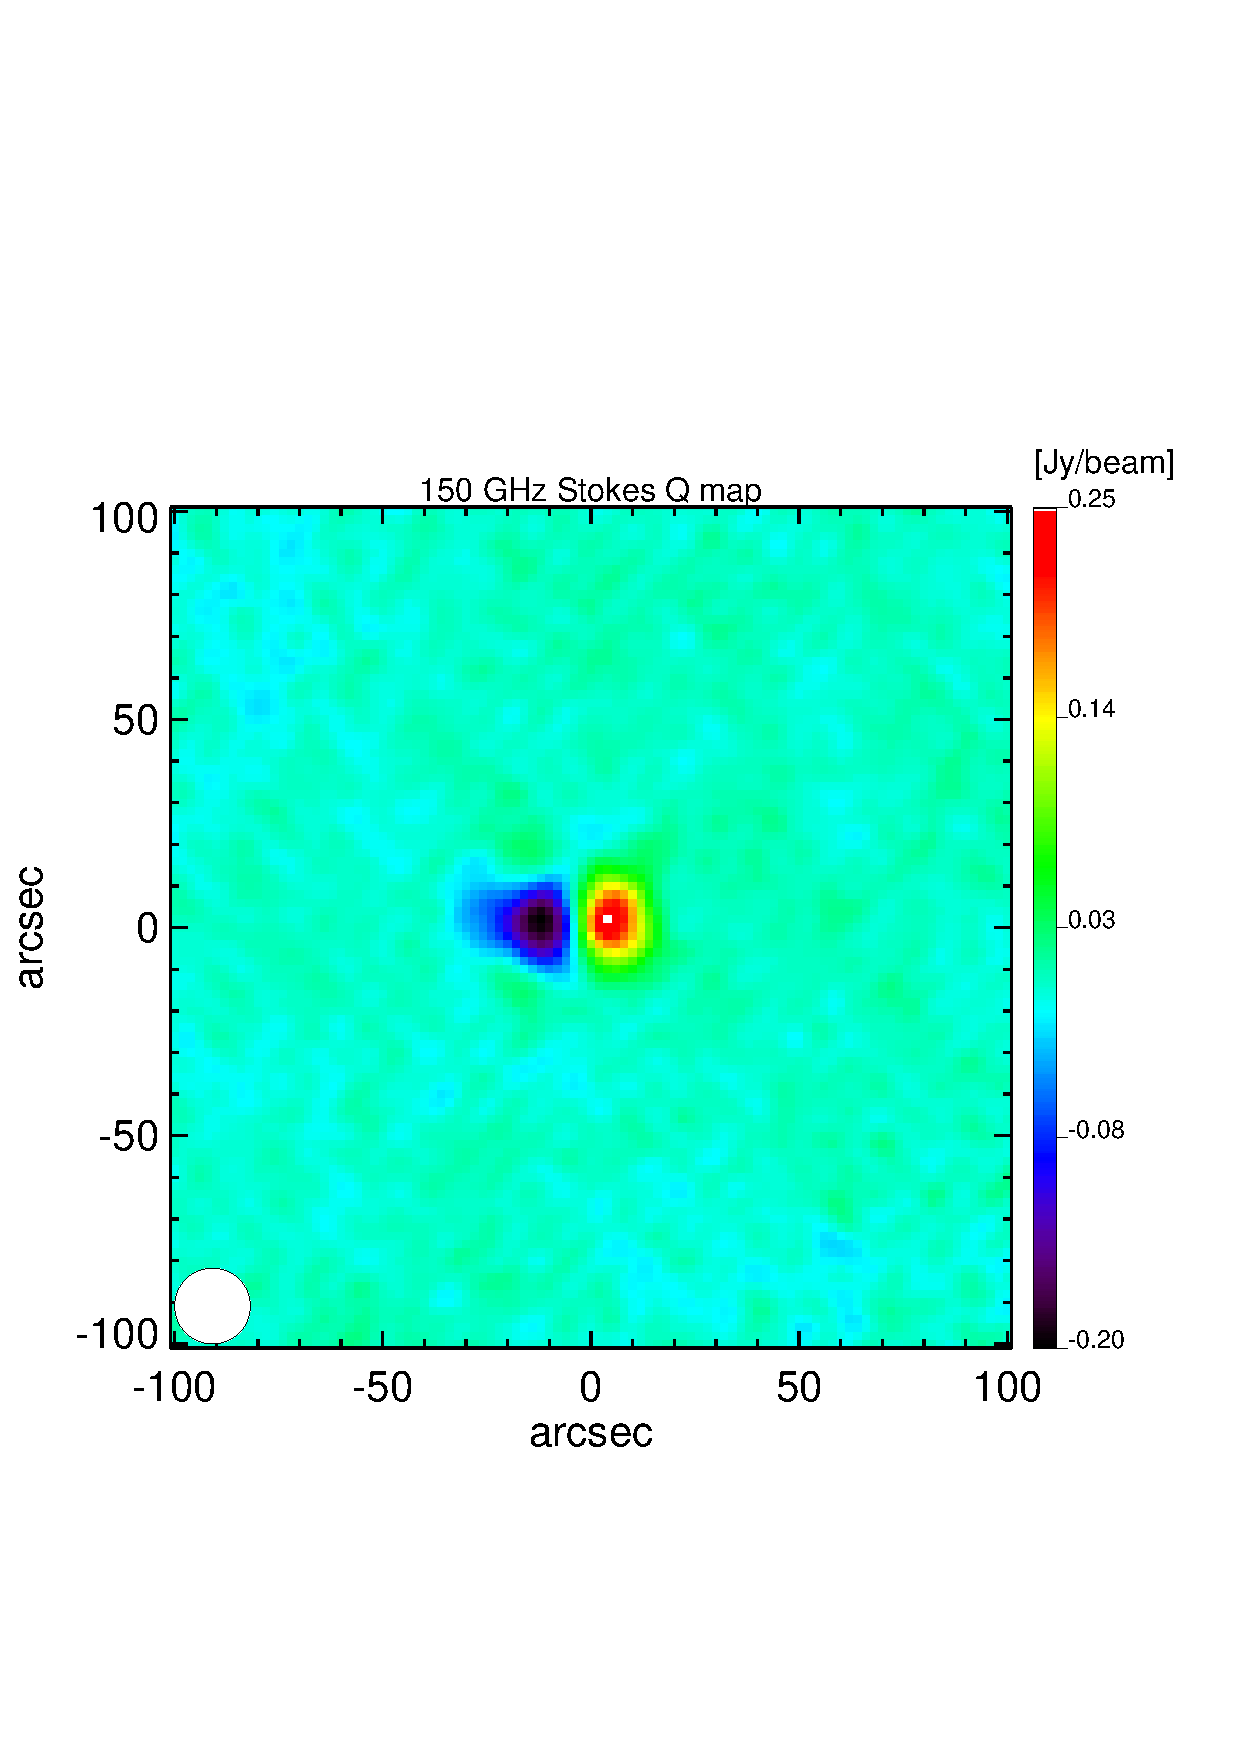
\includegraphics[width=0.33\linewidth,keepaspectratio]{figures/Uranus_Q_map_2mm.pdf}}
     \put(1.4,0.6){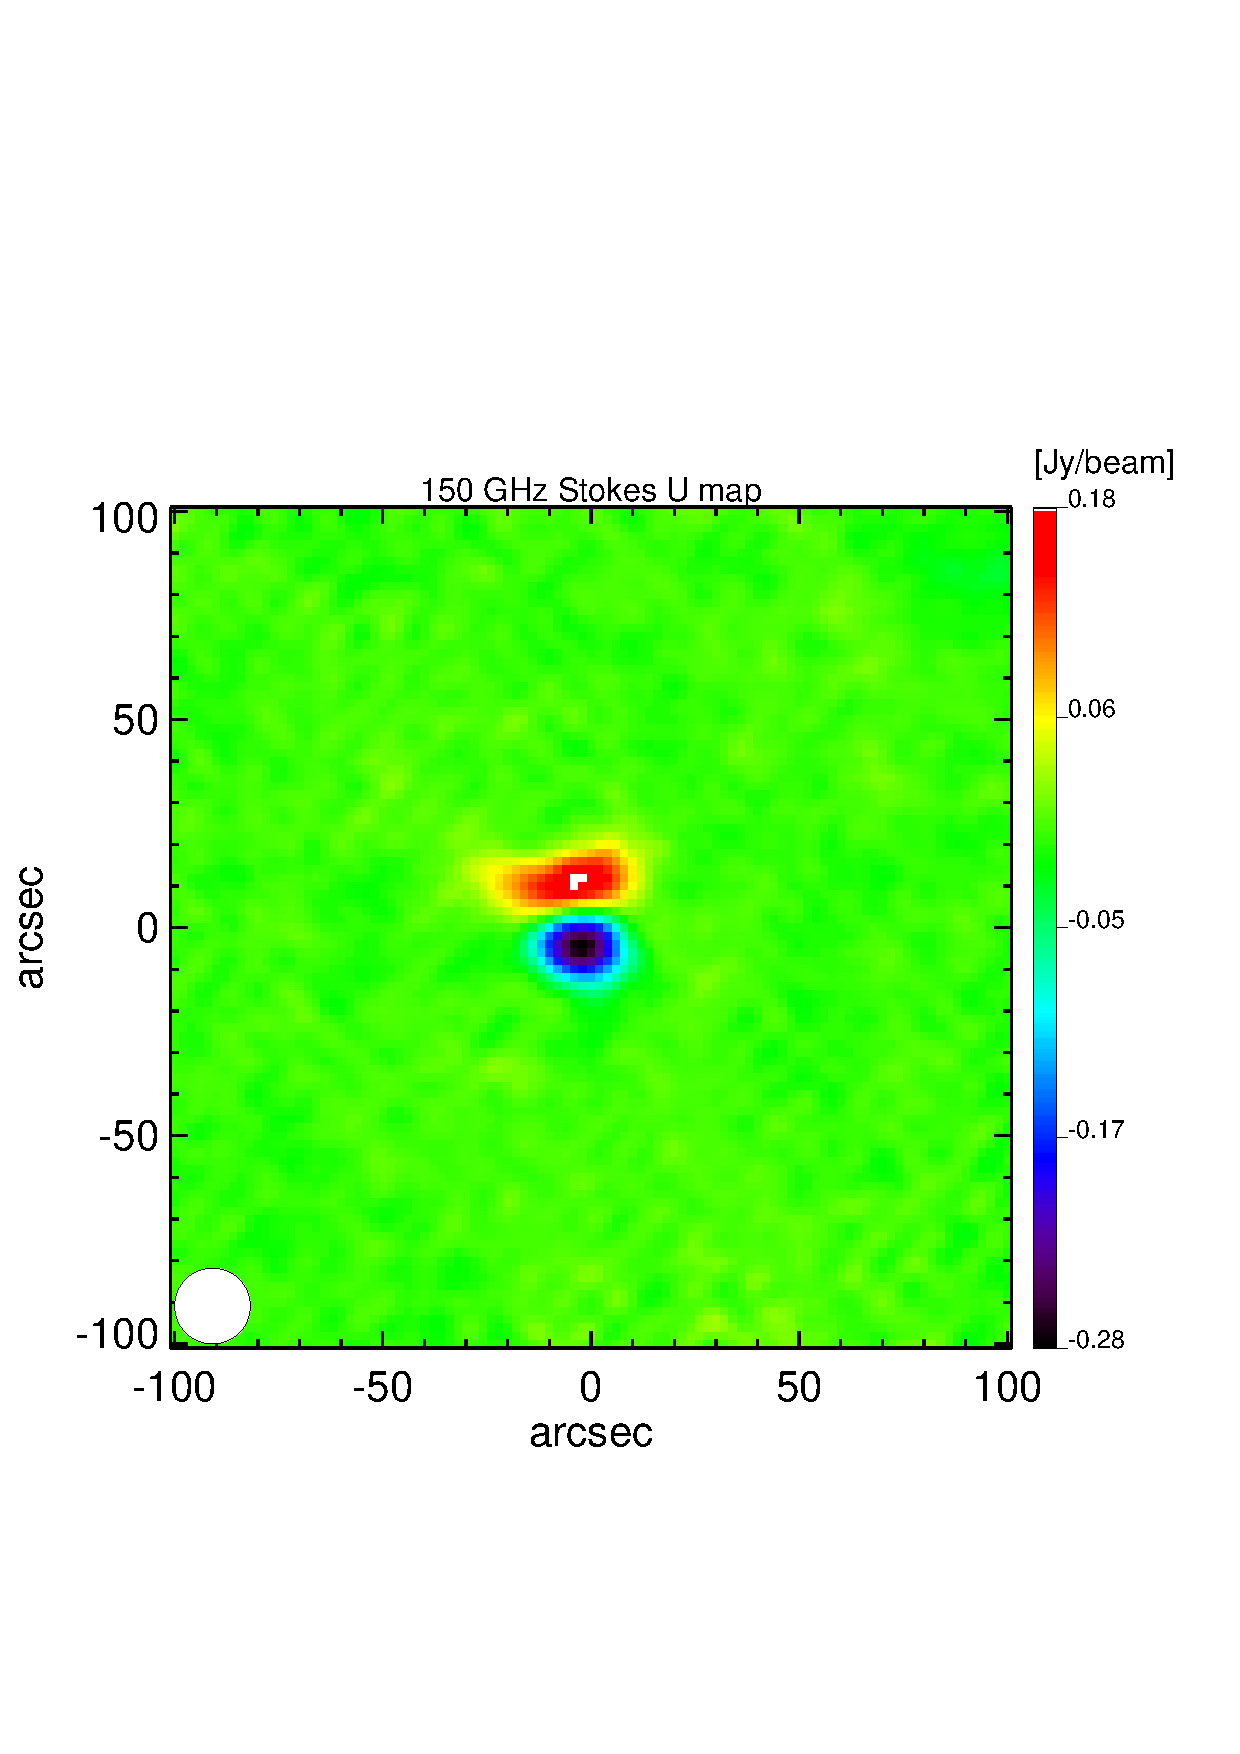
\includegraphics[width=0.33\linewidth,keepaspectratio]{figures/Uranus_U_map_2mm.pdf}}
  %Corrected 2 mm
      \put(0,0){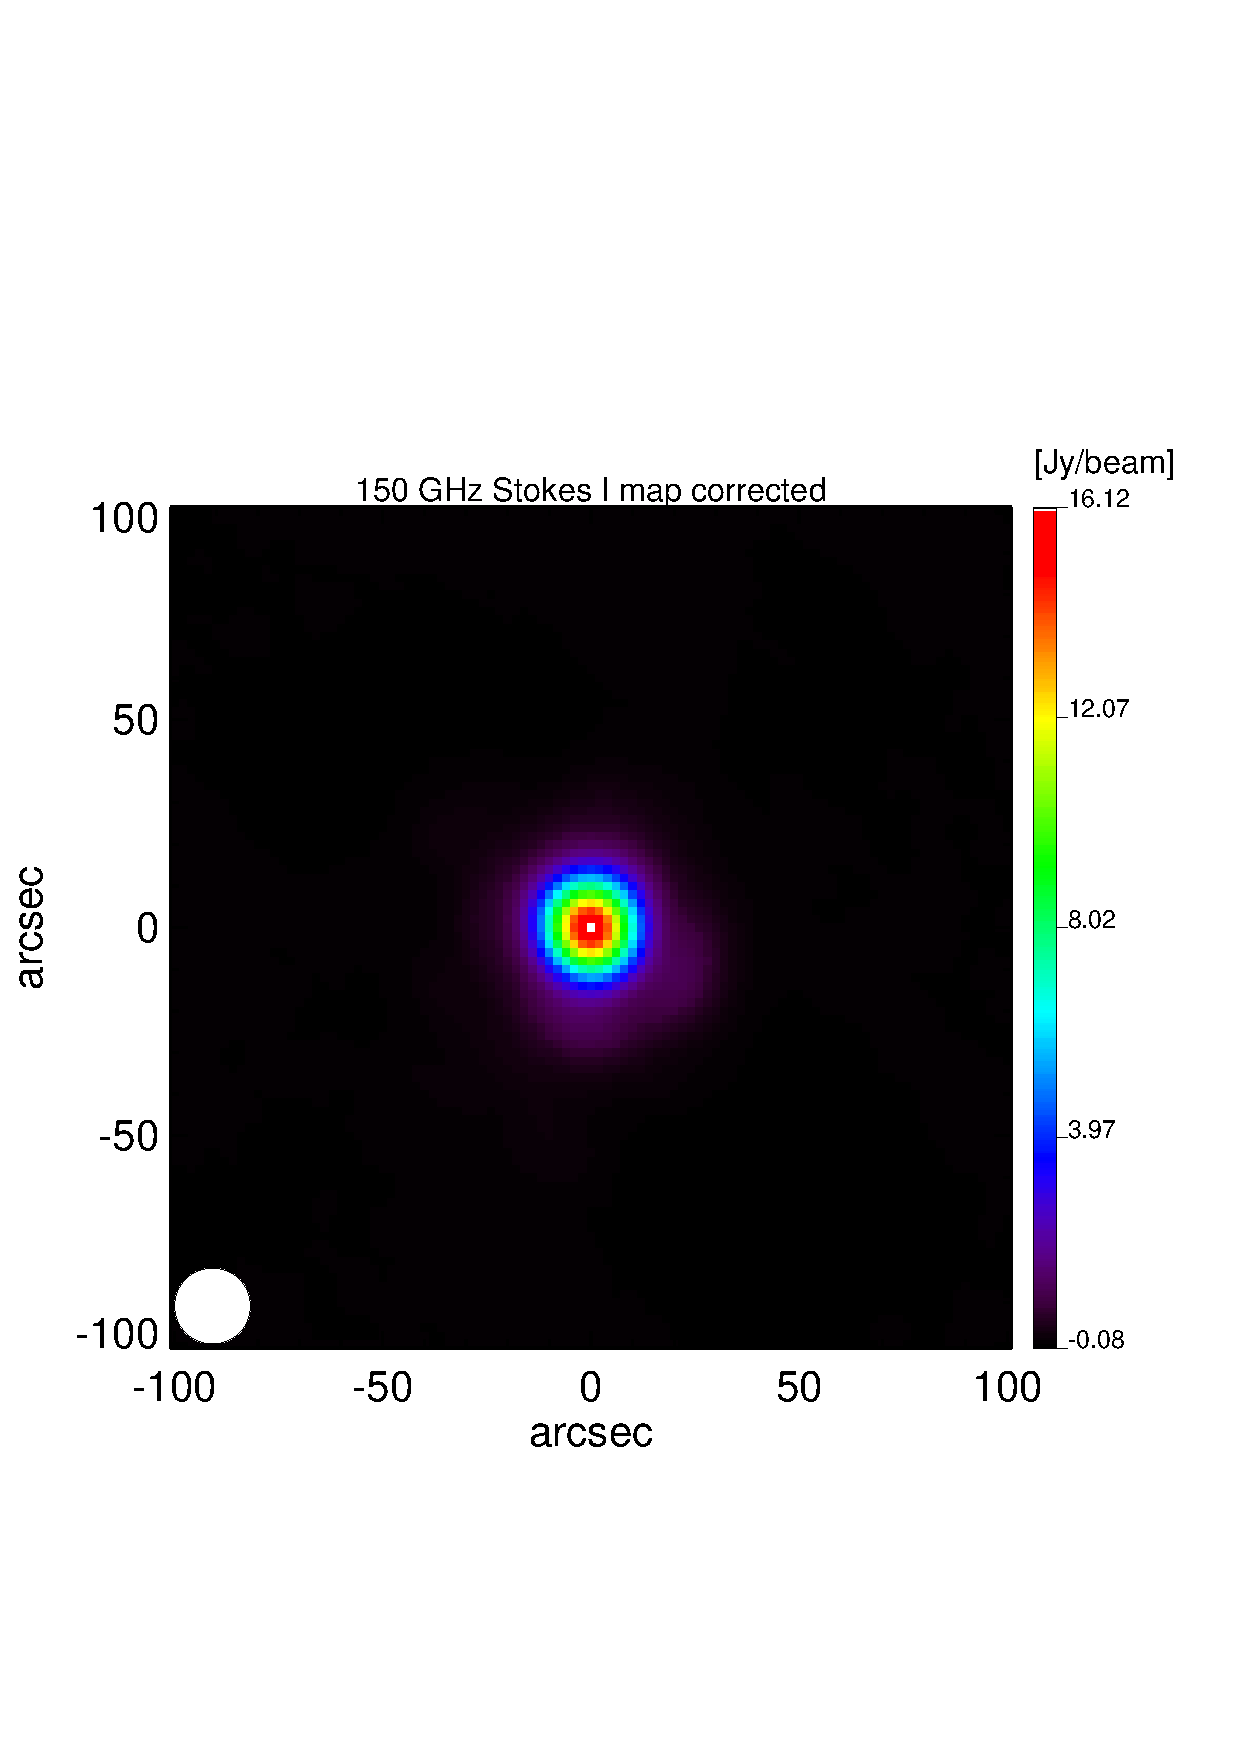
\includegraphics[width=0.33\linewidth,keepaspectratio]{figures/Uranus_I_map_2mm_corr.pdf}}
     \put(0.7,0){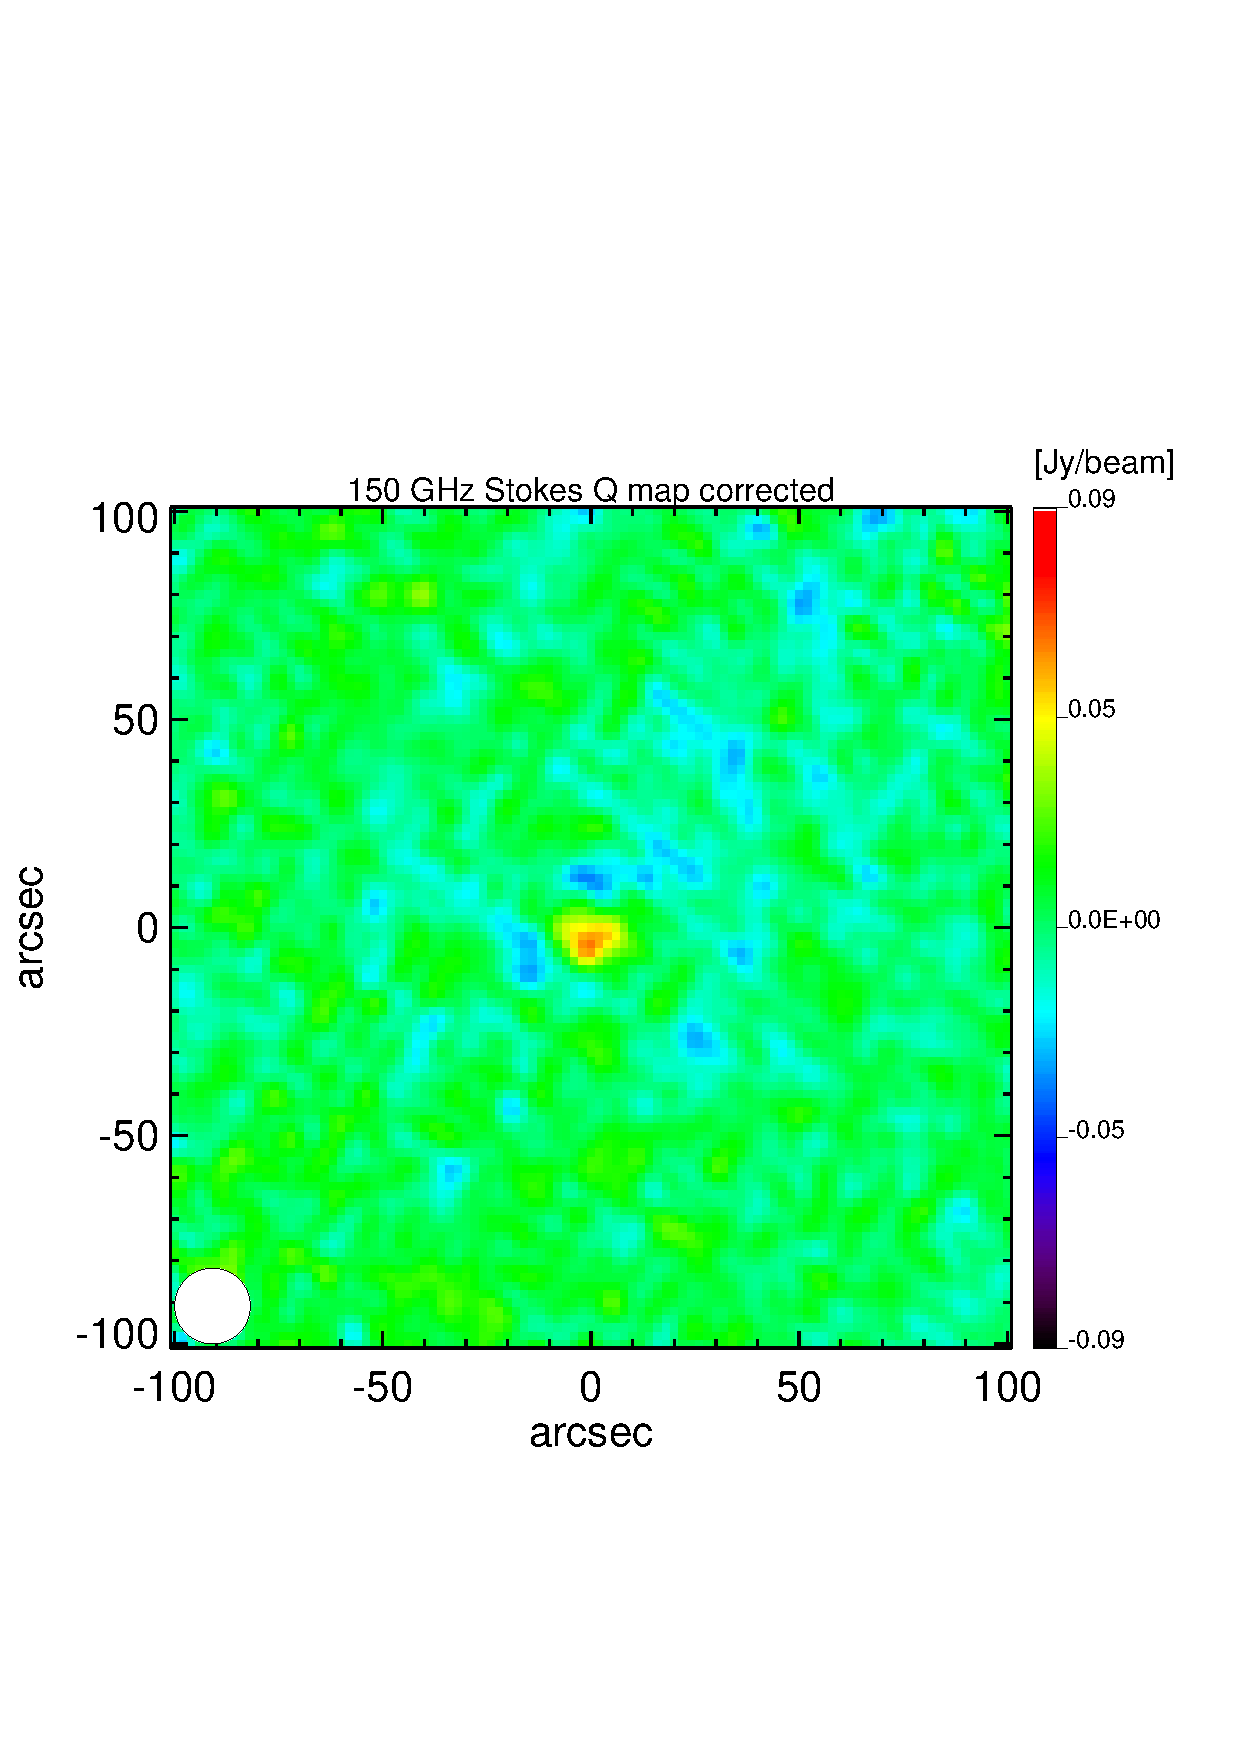
\includegraphics[width=0.33\linewidth,keepaspectratio]{figures/Uranus_Q_map_2mm_corr.pdf}}
     \put(1.4,0){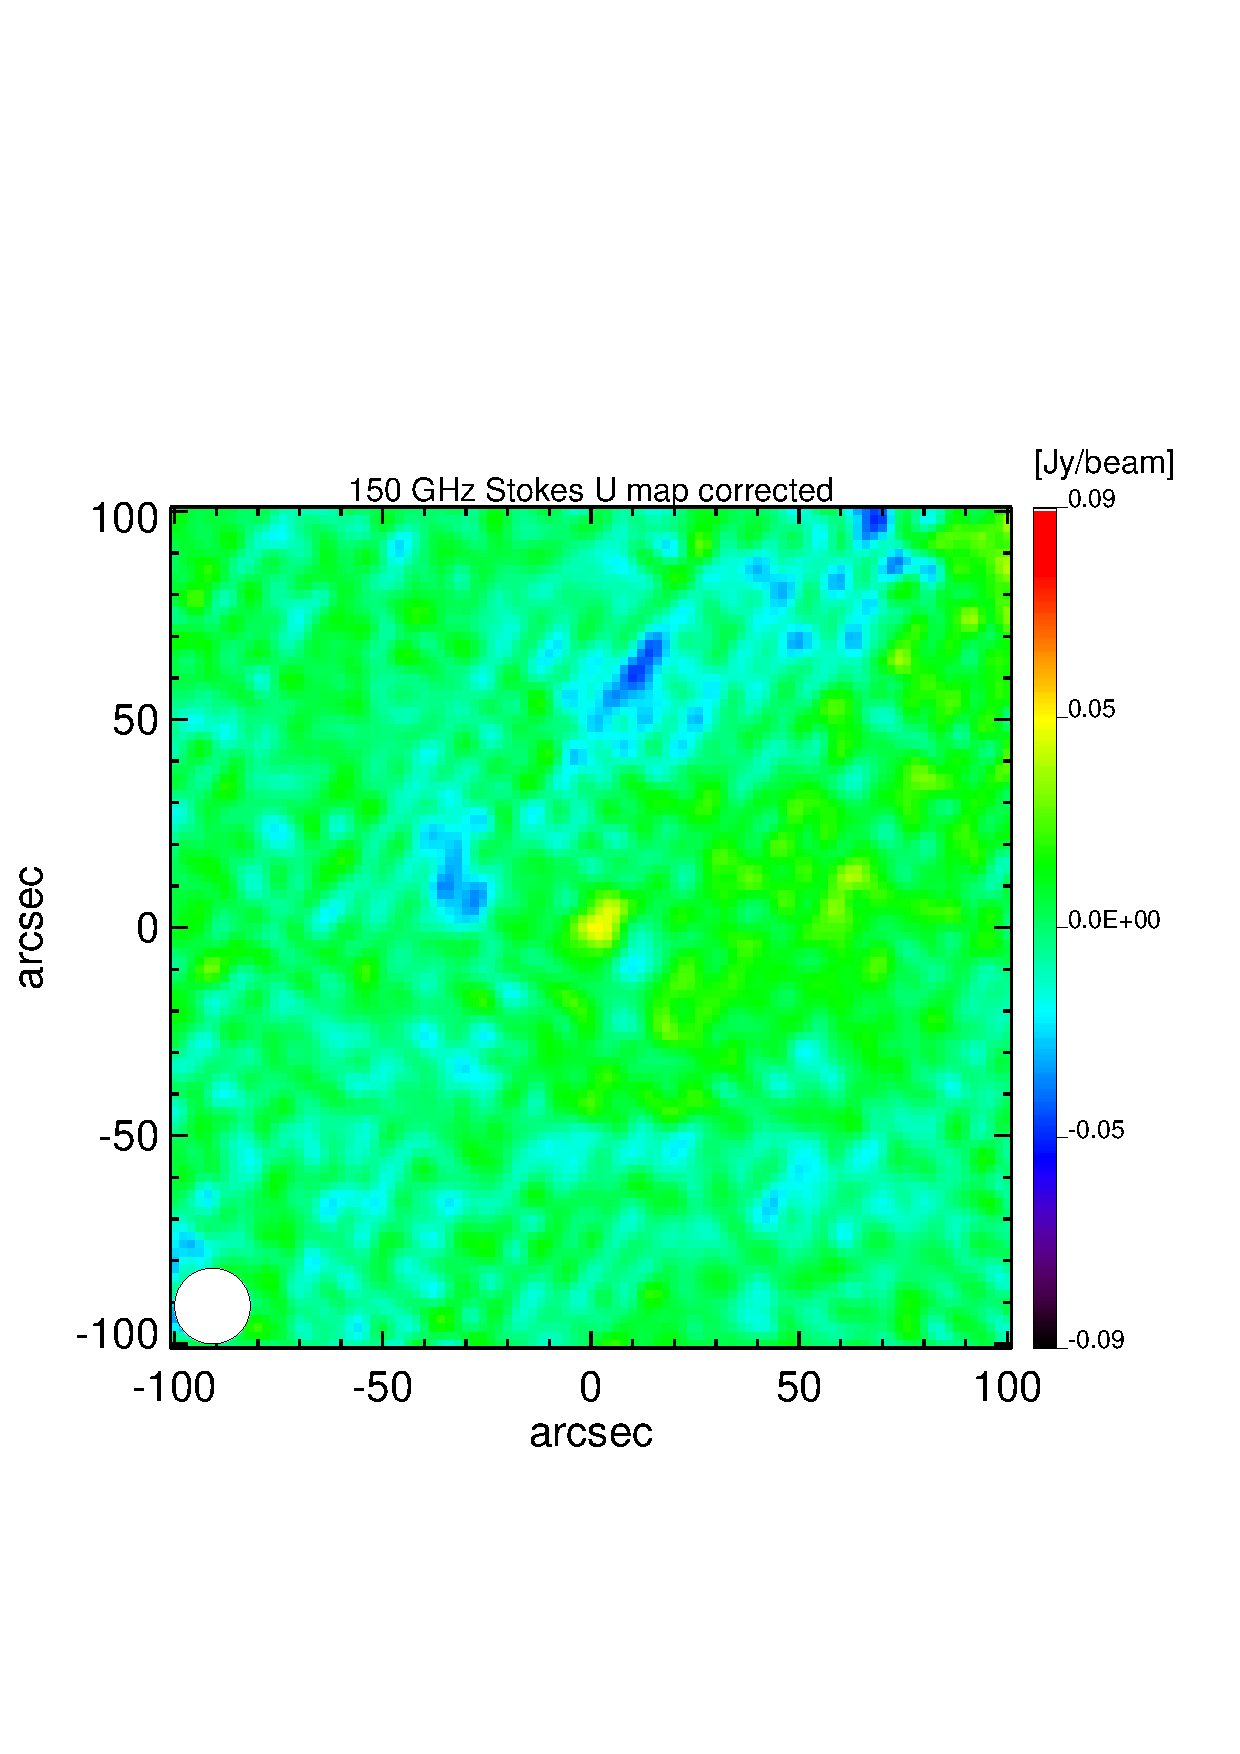
\includegraphics[width=0.33\linewidth,keepaspectratio]{figures/Uranus_U_map_2mm_corr.pdf}}

\end{picture}

  \caption{ Uranus Stokes $I$, $Q$ and $U$ maps in Nasmyth coordinates at 260
    GHz (a) and 150 GHz (b) before and after leakage correction. {\nico dire un
      mot de la polar instrumentale qui reste \`a la fin ici dans la caption et
      montrer qu'on peut la corriger aussi, m\^eme si elle est petite, histoire
      qu'on ne laisse pas croire qu'on ne l'a pas vue...}}
  \label{fig:uranus_lkg}
  \end{center}
\end{figure*}

\begin{figure}
  \begin{center}
     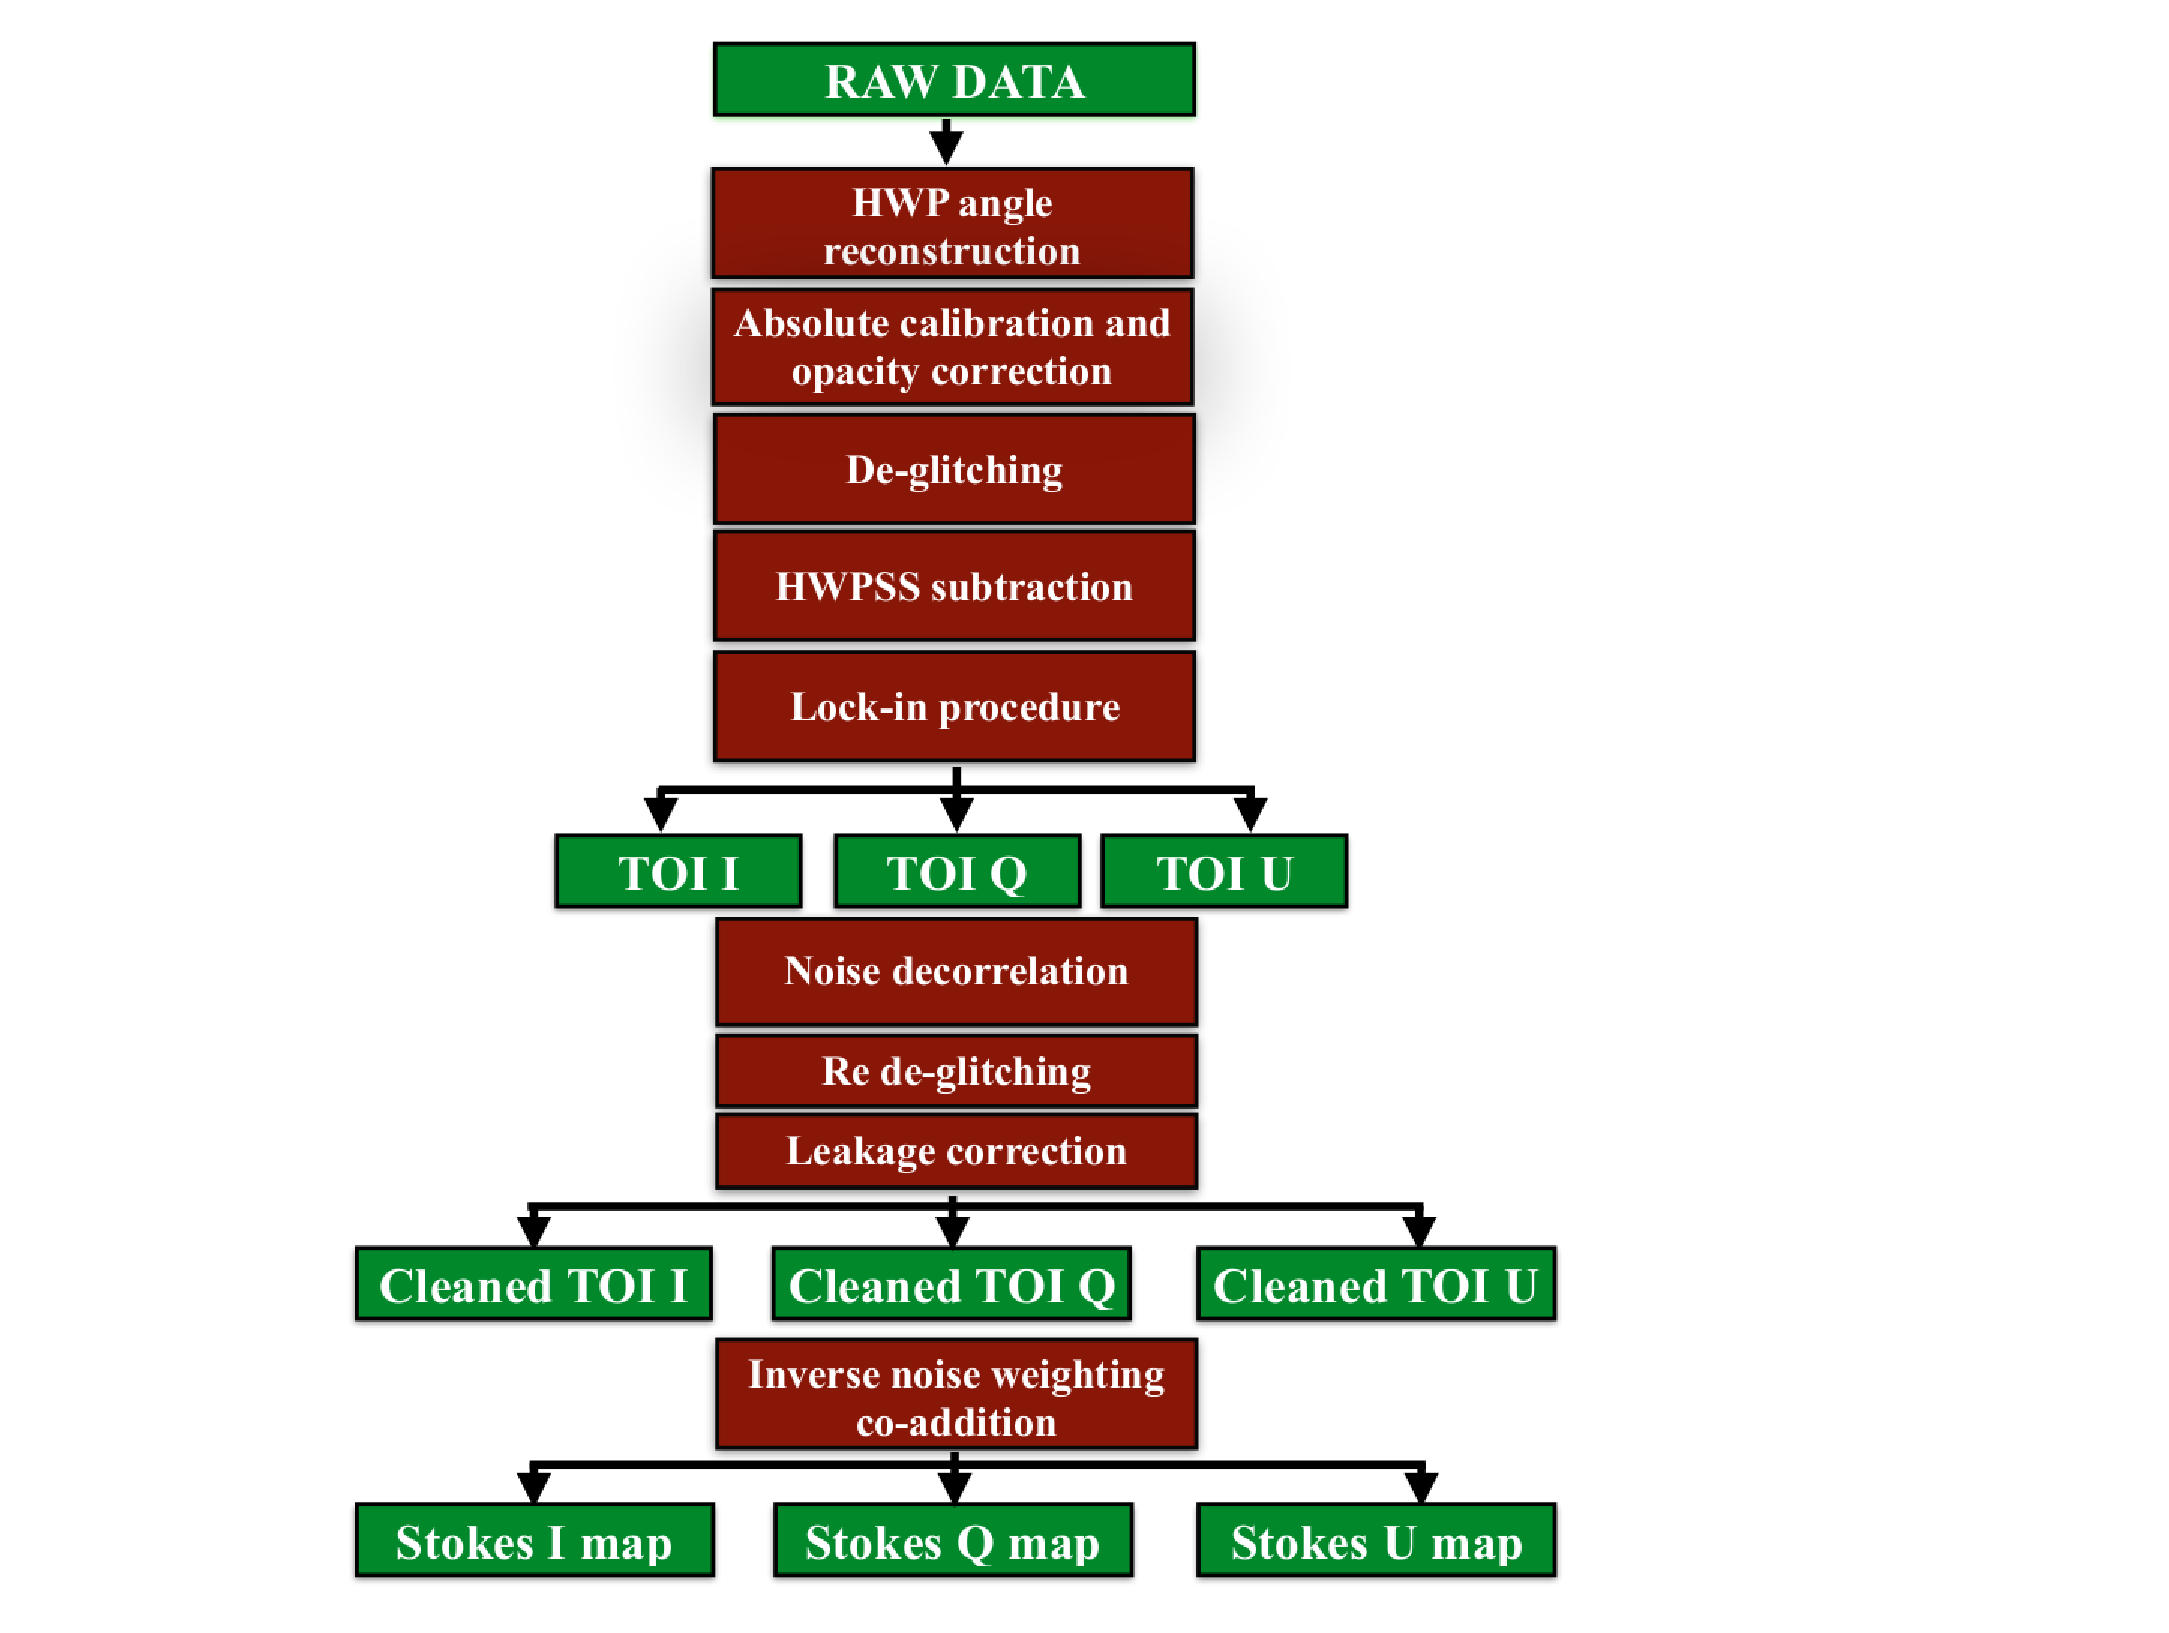
\includegraphics[%
      width=1.3\linewidth,keepaspectratio]{figures/pipeline_scheme_v2.pdf}
\end{center}
\caption{Schematic view of the main procedures of the data processing pipeline from raw data to sky maps. \label{pipe fig}}
\end{figure}

% beginning of Nico's revisions
% beginning of Alessia's revisions
\section{The \nika~ Instrument}
\label{nika instrument}
An extended description of \nika\ {\nico **} and its intensity performances can be found
in \citep{catalano2014, monfardini2010, monfardini2011, Calvo2013}, we here give only a brief
summary of the instrument and focus on the extra module that was added to
provide \nika\ with polarimetric capabilities.

\subsection{\nika: a dual band LEKID camera}
 \nika\ is a dual band camera consisting of two arrays filled by Lumped Element
 Kinetic Inductance Detectors (LEKIDs) with a Hilbert geometry
 \citep{roesch}. LEKIDs are superconducting resonators. When photons are
 absorbed, they break Cooper pairs in the superconducting resonant element. This
 changes the density of quasi-particles and modifies the kinetic inductance, and
 hence the resonant frequency of the LEKID \citep{Doyle2008}. The absorbed power
 can be directly related to the shift of the resonant frequency
 \citep{Calvo2013}. The two LEKID arrays are cooled down to their optimal
 temperature of about 100~mK using a 4K cryocooler combined to a closed-cycle
 $^3$He-$^4$He dilution. The optical coupling between the telescope and the
 detectors is achieved by warm aluminum mirrors and cold refractive optics
 \citep{catalano2014}. The camera observes the sky in two millimeter channels,
 at 1.25 mm and 2 mm corresponding to bandwidths of 220-270 GHz and 137-172 GHz
 with central frequencies of 260~GHz and 150~GHz, respectively. \nika\ has a
 Field of View (FoV) of about 1.8 arcminutes and angular resolutions (FWHM) of
 18.5 arcsec and 12.5 arcsec at 150~GHz and 260~GHz, respectively
 \citep{catalano2014, adam2014}.{\nico we have to decide on 12-18 or 12.5-18.5
   and be consistent.}
 	%The classical design \citep{monfardini2011} was sensitive to the polarization, therefore the efficiency of the imaging experiment was reduced. So it has been chosen a new design, the LEKID Hilbert geometry \citep{roesch} that make the pixels sensitive to both orientations of the linear polarization.

%	\subsection{NIKA POLARIMETER} 

\subsection{The polarimetric module}
\label{sec:pol_module}


%\begin{figure}
% \begin{center}
%   \includegraphics[width=6cm, keepaspectratio]{figures/SETUP.pdf}
%    \caption{ Laboratory instrumental setup. From left to right,
%     the {\it NIKA} cryostat, the HWP in a fixed position and a Martin-Puplett
%      interferometer.}
%    \label{fig:setup_lab}
%  \end{center}
%\end{figure}

The polarization setup of the \nika\ camera consisted of a continuously rotating
HWP and an analyser, at room temperature, facing the \nika\ camera window. The
Hilbert geometry \citep{roesch} of the \nika\ LEKIDS was specifically optimized
for intensity observations and as a consequence \nika\ LEKIDs were not sensitive
to polarization. Therefore, for polarization observations an analyser was placed
after the HWP at a distance of 6 cm of the cryostat window as shown in the two
configurations of Figure~\ref{polarsetup}. The analyser, consisting of a
lithographic kapton coper polarimeter, was {\nico tilted by 10 degrees} with
respect to the optical axis to avoid standing waves with the cold optical
filters inside the cryostat. The HWP was placed before the analyser {\nico and
  shared} the same holder.  We used a hot-pressed metal mesh HWP designed and
built at Cardiff University \citep{pisano}. The HWP was especially designed to
allow {\nico an} approximately constant phase shift of the transmitted radiation
over a broad spectral band including the two \nika\ bands. A two-layer broadband
anti-reflection coating was added to the HWP to maximize the transmission across
the band. The HWP was mounted into a mechanical modulator actioned by a stepper
motor synchronously controlled by the \nika\ acquisition system. The power of
the motor was chosen so that a typical stable rotation frequency of 5~Hz could
be achieved during observational campaigns of at least one week. We chose a
Sanyo Denki 103H8221-5141, which is a 2-phase stepping motor.

The combined action of the continuously rotating HWP and the analyser leads to a
modulation of the input linear polarization at four times the mechanical
rotation frequency, $\omega_{\rm P} = 2 \pi \nu_{P}$. Thus, letting aside
calibration and system imperfections, each LEKID in the focal plane measures the
following combination of the three Stokes parameters
\begin{equation}
m = I + \rho_{\rm pol} \lbrace Q \cos ( 2 \psi(t) + 4 \omega_{\rm P} \ t) + U \sin ( 2\psi(t) + 4 \omega_{\rm P} \ t) \rbrace.
\label{photoequ}
\end{equation}
$\psi(t)$ is the angle between the analyser and the {\nico ``reference'' rather
  than horizontal (it
  actually is vertical in most cases :)} axis of the polarization reference
frame {\nico i.e. the direction along which $U=0$ and $Q>0$.}
$\rho_{\rm pol}$ is the polarization efficiency of the full system. 
{\nico I also suppress the sentence about the Nasmyth ref frame. At this stage,
  we are more general than this and the equation stands for any reference frame,
radec, nasmyth, azel}
%which was set perpendicular to the light propagation direction in the cabin Nasmyth reference frame.


% \nika~LEKIDs
%are sensitive to both polarizations and the polarizer placed behind the HWP
%plays the role of an analyser. It is rotated at constant pace by a stepper motor
%({\color{red} give a bit more details on this rotator...}
  
%%%\begin{figure}[h!]
%%\begin{figure}
%% \begin{center}
%%\includegraphics[width=8.5cm, , keepaspectratio]{figures/setup_polar.png}
%%\caption{ Observational polarimeter scheme. From left to right we
%%  observe the rotating HWP, the polarizer and the {\it NIKA} cryostat containing
%%  the arrays of LEKID detectors.}
%%\label{fig:setup_polar}
%%\end{center}
%%\end{figure}

\section{Laboratory characterisation of the polarimetric module}
\label{sec:lab_characterisation}

%\begin{figure}[h!]


%{\color{red}
%\begin{itemize}
%\item[-] {\color{green} the ``cryostat'' used in these lab tests actually was \nika, right
%  ? let's mention it then and rephrase the sentence. {\color{cyan} non, it was not.}}
%\item[-] need to add a word on what was done in Cardiff and
%  why we do or do not report on this here.
%\item[-] Need to justify what previous experience allows us to assume that the
%  polarizer is perfect.
%\item[-] I don't understand why we talk about distortion of the bandpass with
%  the HWP rotation ? Do you mean ``attenuation'' instead ?
%\item[-] {\bf We need to explicit an equation to explain why it's a 45 deg
%  rotation that separates max and min transmissions (add formula somewhere somehow)}
%\item[-] I've removed the mention to the ``linear shift'' between the two bands
%  because it's not shown on any plot and not dicussed. If we do have sthg to say
%  about this, we should develop more. We should definitely say and show that the
%  HWP is achromatic.
%\end{itemize}
%}
We start this section by introducing the main parameters used in the
characterisation of the \nika\ HWP. {\nico Following Savini et al XXX}, the
Mueller matrix of a general realistic HWP can be written as

\begin{strip}
 %\begin{widetext}
  \begin{eqnarray} \label{equ.HWP}
%    \begin{split}
      M_{HWP}=\frac{1}{2} \left(\begin{array}{lll} \\
        \alpha^2+\beta^2              & (\alpha^2-\beta^2)\cos2\theta & (\alpha^2-\beta^2)\sin2\theta \\
        (\alpha^2-\beta^2)\cos2\theta & (\alpha^2+\beta^2)\cos^22\theta +
        2\alpha\beta\sin^22\theta\cos\phi &
        (\alpha^2+\beta^2-2\alpha\beta\cos\phi)\cos2\theta\sin2\theta \\
        (\alpha^2-\beta^2)\sin2\theta &
        (\alpha^2+\beta^2-2\alpha\beta\cos\phi)\cos2\theta\sin2\theta &
        (\alpha^2+\beta^2)\sin^22\theta + 2\alpha\beta\cos^22\theta\cos\phi
%        \label{eq:mueller_mat}
      \end{array}\right)
   % \end{split}
  \end{eqnarray}

%\end{widetext}
\end{strip}

\noindent {\nico ** $\alpha$ and $\beta$ **} represent the normalised
transmission coefficients on the ordinary and extraordinary axes of the HWP.
The HWP phase shift angle between the ordinary and extraordinary axes is noted
as $\phi$.  $\theta$ represents the angle of the HWP ordinary and extraordinary
axes with respect to the polarization reference frame.

A first characterisation of the properties of the \nika\ HWP was carried out
after fabrication at Cardiff University. In particular the HWP phase shift angle
$\phi$ was measured over the full bandwidth from 100 to 350~GHz as shown in the
top panel of Figure~\ref{fig:spectre}.
%pour trouver maximum on prend trois spectre dans la region maximale et puis on prend le plus haut 
%{\color{red} \bf alpha et beta : 8 spectres a difference angles
%nombre de pas MPI: 80
% spectral resolution of about 3.5GHz (about 44 mm of excursion of the roof mirror)
%temps de me sure: 9.16 min
%characterisation axes optique ->  mesures int�gres sur la bande et on a cherche le maximum et le minimum}
Furthermore, in order to estimate the performance of the whole polarization
chain, we performed laboratory measurements of the system transmission.  We used
a polarizing Martin Puplett Fourier Transform Spectrometer (MPFTS) to
characterize the spectral transmission of the system.  The MPFTS produces the
difference between the power of two input polarized beams that come from two
black bodies at different temperatures (ambient eccosorb and warmed eccosorb)
modulated by a rotating wire-grid polarizer.  An array of LEKIDs was placed
facing the MPFTS inside a \nika\ type dilution cryostat, which cools down the
optics, the analyser and the LEKIDs to 100 mK.  The analyser consists of a
wire-grid and it will be considered as ideal in the following.  A schematic
view of the instrumental setup is shown on the left panel of
Figure~\ref{polarsetup}.

We have performed a total of eight independent measurements by varying the angle
of the \nika\ HWP axis with respect to the optical axis.  For each transmission
measurement the HWP was kept fixed during data taking. We achieved a spectral
resolution of about 3.5 GHz, which corresponds to about a 44 mm excursion of the
roof mirror of the MPFTS. We covered the bandwidth of interest by considering a
total of 80 steps by transmission measurement for total of 9 minutes of
integration time.  As the MPFTS polariser and the analyser transmission axis
were set perpendicularly to each other, prior to any measurement we rotated the
\nika\ HWP to find a zero point initial position, which maximized the measured
LEKID signal.  By rotating the HWP for each measurement we rotated the
polarization of the MPFTS output signal.  As the analyser was kept at fixed
position, this induced an attenuation of the signal measured by the LEKIDs.
This can be observed in the bottom panel of Figure~\ref{fig:spectre} where we
present the measured transmission as a function of frequency for four HWP
positions going from the maximum (black solid line) to the minimum of
transmission (dashed solid line) spectra.  As expected the relative HWP angle
between the maximum and minimum transmission is about 45 degrees.{\nico why
  don't we say compatible within our uncertaintites with the expected 45 degrees ?}
%When the HWP
%aligns the polarization with the analyser, we have maximum transmission ($46.8
%\pm 1.8^{\circ}$), when it aligns it in the orthogonal direction, we have
%minimum transmission ($86.4\pm1.8^\circ$). The nearly $45^\circ$ difference
%between these two HWP positions agrees with
%Eq.~(\ref{eq:hwp_and_polarizer}). Note that we cannot expect zero transmission
%because of the wide band of the instrument ({\color{red} Please confirm this or
%  give explanations why we do not measure strictly 45 deg within error bars :)
%  Actually, the absolute error is not 1.8 deg but 3.6 deg, which is now
%  compatible with the 5 deg difference between 45 theoretical and 40 measured,
 % but we need to make clear in the paper, that the stepper motor is very well
 % controlled and that the error on each individual angle is much less than 3.6
%  deg.}. 

We used previous transmission spectrum measurements to determine
the $\alpha$ and $\beta$ transmission coefficients describing the HWP.
Taking as a reference the maximum transmission spectrum described above,
we fit for the other transmission spectra taken at different angles of the HWP
with respect to the reference polarization axes. We assumed the 
HWP model in Equation~\ref{equ.HWP} and accounted for the analyser facing
the LEKID array. The phase shift angle, $\phi$, was set to the values per frequency measured
at Cardiff University and presented above.
%birefringent axes. $\theta$ is the angle of the incident polarization with
%respect to the reference frame defined by these axes and {$\phi$} is the phase
%shift introduced by the plate between the two orthogonal polarizations. $\phi$
%is a vector of values found during the simulations carried out by Cardiff group
%when the HWP was manufactured in order to optimize the trasmission of the
%polarized light. 
Notice that as we are using the maximum transmission
spectrum as a template we are not sensitive to an overall attenuation amplitude.
Therefore, to simplify the procedure we fixed $\alpha$ to one and we
only fitted for $\beta$. Using a least square minimisation we find $\beta = 0.994\pm0.005$ at 1.25
mm and $\beta = 0.924\pm0.005$ at 2 mm. The best fit models obtained for each position
of the HWP are plotted in red in Figure~\ref{fig:spectre}.

Defining the polarization efficiency as $\rho_{pol} = (1-2\gamma)/2$ where
$\gamma = \frac{\alpha \beta \cos(\phi)}{\alpha^2 + \beta^2}$ we find $\rho_{\rm
  pol} = 0.994 \pm 0.01$ at 1.25 mm and $0.986 \pm 0.01$ at 2 mm. These values
are accounted for in the final absolute calibration of our polarization
maps. Finally, as a consequence of the small difference observed between the
$\alpha$ and $\beta$ transmission coefficients we expect the modulation the
incoming intensity and polarization around the second harmonic of the HWP
rotation ({\nico see Fig.}~\ref{spectre_iqu}). However, as presented in Sect.~\ref{se:demod_mapmaking}, we are not
sensitive to this effect in the final maps as it is accounted for in the data
processing.
%% of the for each wavelength due to the linear relation
%% between the phase shift and the wavelength. This effect is expected to be quite
%% weak because the HWP is achromatic \citep{moncelsi2014}. First we measured a
%% spectrum with the HWP aligned to its ordinary axis. This corresponds to the
%% maximum signal in which we expect to have no distortion {\color{red} see
%%   comment} of the {\it NIKA}
%% bandpass, as measured in intensity \citep{catalano2014}. This is taken as a
%% reference spectrum. Rotating the HWP we found an attenuation as shown in
%% fig. \ref{fig:spectre}, here the maximum transmission is represented by the
%% spectrum at about 46.8$^{\circ}$ $\pm$ 1.8$^{\circ}$ with respect to the HWP
%% zero.

% The polarized transmission is therefore of $\sim$ 100\% in the {\it NIKA} band
% frequency with a polarized transmission loss of 0.6 $\%$ in the 1mm channel and
% of 1.4$\%$ in the 2mm channel.
 
%In the 1mm channel the polarization loss is very low so we consider to work with
%an ideal HWP assuming the $\rho_{pol}$ = 1 in the following data reduction
%analysis. In the 2mm channel we take into account for the coefficient
%$\rho_{pol}$ in the calibration factor.

%\landscape
\begin{table*}
%\begin{landscape}
\begin{center}
\caption{\nika\ measured intensity and polarization fluxes, polarization degree and angle at 260 GHz and at 150 GHz for the quasars observed during the February 2015 campaign. }

%\begin{tabular}{ccccccccccccc}
\begin{tabular}{ccccccccc}
\hline
\hline
Source & Frequency & I flux & Q flux &  U flux  & p & $\chi$  \\ %& I flux & Q flux &  U flux  & p & $\psi$ \\
            & [GHz]         & [Jy] & [Jy] & [Jy] & [\%] & [$^\circ$] \\ % & [Jy] & [Jy] & [Jy] & [\%] & [$^\circ$] \\
%            & 260 GHz & 260 GHz & 260 GHz & 260 GHz & 260 GHz & 150 GHz & 150 GHz & 150 GHz & 150 GHz & 150 GHz\\
\hline
\hline
3C279 & 260 &  8.51$\pm$0.97 &  0.260$\pm$0.005 & 0.79$\pm$0.09 & 9.8 $\pm$ 2.2 & 35.9$\pm$1.4(stat) $\pm$1.8(syst)  \\
            & 150 &  12.4$\pm$1.4 &  0.51$\pm$0.06 &  1.05$\pm$0.12 &  9.5$\pm$2.2 & 31.9$\pm$1.8(stat)$\pm$1.8(syst) \\
\hline
3C273 & 260 &  6.3 $\pm$0.7 & -0.22 $\pm$ 0.01 & -0.009 $\pm$0.001 &  3.8$\pm$0.4 & -88.6$\pm$0.2(stat)$\pm$1.8(syst) \\
            & 150 & 10.04 $\pm$1.12 & -0.17$\pm$ 0.02 & -0.10$\pm$ 0.01 &  2.0 $\pm$ 0.5 & -74.1 $\pm$ 2.1(stat) $\pm$ 1.8(syst) \\
\hline
3C286 & 260 &  0.27$\pm$0.03 & 0.020$\pm$0.002 & 0.033$\pm$0.004 & 14.1$\pm$3.2 & 29.0$\pm$2.1(stat) $\pm$ 1.8(syst) \\
            & 150 & 0.51$\pm$0.10 & 0.037$\pm$0.004 & 0.05$\pm$0.01 & 12.9$\pm$2.9 &  27.7$\pm$2.1(stat) $\pm$ 1.8(syst) \\
\hline
3C345 & 260 &  1.08$\pm$0.12 & 0.035$\pm$0.002 & 0.003$\pm$ 0.004 & 3.2$\pm$ 0.7 & 2.7$\pm$0.4(stat) $\pm$ 1.8 (syst ) \\
            & 150 &  1.82 $\pm$ 0.20 & 0.031$\pm$0.003 & 0.010$\pm$0.001 & 1.8$\pm$0.4 &  9.2$\pm$1.4(stat) $\pm$ 1.8(syst) \\
\hline
1749+096 & 260 & 1.64$\pm$0.19 & 0.005$\pm$0.004 & 0.063$\pm$0.007 &  3.9$\pm$0.9 & 43.0$\pm$0.3(stat) $\pm$ 1.8(syst) \\
	         & 150 & 1.93$\pm$0.20 & -0.0016$\pm$0.0002 & 0.07$\pm$0.01 & 3.6$\pm$0.8 & 45.6$\pm$ 0.1(stat) $\pm$ 1.8(syst)  \\
\hline
0851+202 & 260 & 3.27$\pm$0.37 & -0.105$\pm$0.002 &  0.02$\pm$0.002 & 3.3$\pm$0.7 & 84.0$\pm$0.9(stat) $\pm$ 1.8(syst)  \\
                 & 150 &  4.36$\pm$0.51 & -0.10$\pm$0.01 & 0.08$\pm$0.01 & 2.9 $\pm$ 0.7 & 70.3 $\pm$2.3(stat) $\pm$ 1.8(syst)  \\
\hline
0923+392 & 260 & 2.04$\pm$0.23 & -0.002 $\pm$0.005 & -0.07 $\pm$ 0.01 & 3.3$\pm$0.7 & -45.8$\pm$0.1(stat) $\pm$ 1.8(syst) \\
                 & 150 & 3.25$\pm$0.41 & -0.016$\pm$0.002 &  -0.09 $\pm$ 0.01 & 2.7$\pm$0.6 & -50.3$\pm$0.8(stat) $\pm$ 1.8(syst)  \\
\hline
0415+379 & 260 & 1.29$\pm$0.15 & 0.017$\pm$0.006 & -0.025$\pm$0.003 & 2.4$\pm$0.5 &  -28.4$\pm$2.1(stat) $\pm$ 1.8(syst) \\
                 & 150 & 1.8$\pm$0.2 & 0.010$\pm$0.001 & -0.028$\pm$0.003 & 1.7$\pm$0.4 & -34.2$\pm$1.6(stat) $\pm$ 1.8(syst)\\
\hline
\end{tabular}
\label{tab:table_quasar}
\end{center}


%\begin{center}
%\caption{ Results of the parallel session of observation between XPOl and {\it NIKA} for polarization degree and angle for the quasars 3C273, 1749+096, 0851+202, 0415+379. The {\it NIKA} angle uncertainty takes into account for both statistical and systematic error.}
%\begin{tabular}{cccccccccccc}
%\hline
%\hline
%Source & p  & p  & p  & p  & $\psi$ & $\psi$ & $\psi$  & $\psi$\\
 %& [$\%$] & [$\%$] & [$\%$] & [$\%$] & [$^\circ$] &[$^\circ$] &[$^\circ$]&[$^\circ$] \\
% & {\it NIKA} 1.25 mm & {\it NIKA} 2.05 mm & XPOl 1.3 mm & XPOl 3 mm & {\it NIKA} 1.25 mm  & {\it NIKA} 2.05 mm & XPOl 1.3 mm & XPOl 3 mm \\
 
%\aline
%3C273 & 3.8$\pm$0.4       & 2.0 $\pm$ 0.5 & 3.6$\pm$ 0.2  & 1.1$\pm$ 0.1 & -88.6$\pm$2.0 & -74.1 $\pm$ 3.9  & -76.8$\pm$ 1.6 & -37.8$\pm$ 0.9\\
%1749+096 & 3.9$\pm$0.9 & 3.6$\pm$0.8 & 2.0$\pm$0.3      & 0.9$\pm$0.1 &  43.0$\pm$2.1 & 45.6$\pm$ 1.9 & -83.0$\pm$3.7 & 75.0$\pm$1.6 \\
%0851+202 & 3.3$\pm$0.7 & 2.9 $\pm$ 0.7 & 2.8$\pm$0.3    & 1.1$\pm$0.1 & 84.0$\pm$2.7 & 70.3 $\pm$4.1 & -67.5$\pm$2.4  & -38.5$\pm$1.7 \\
%0415+379 & 2.4$\pm$0.5 & 1.7$\pm$0.4 & 2.2$\pm$1.5     & 0.4$\pm$0.1 & -28.4$\pm$3.9  & -34.2$\pm$3.4 & 74.2 $\pm$19.3  & -14.2 $\pm$7.2\\
%\hline
%\end{tabular}
%\label{tab:calib_degree}
%\end{center}

\begin{center}
\caption{Degree and angle of polarization of the \nika\ observed quasars as measured by external experiments.}
\begin{tabular}{ccccccccc}
\hline
\hline
Source & Experiment & Wavelength & p & $\chi$ & Observation date & Comments\\
 & & & $[ \%]$&[$^\circ$]\\
\hline
\hline
3C279 &  SHARP Polarimeter &  350 $\mu$m, (3.5, 7, 13) mm &  10 $\%$-12 $\%$ & 32-41 &  2014, March & Variable source\\
           &  XPOL & 1.25 mm & 11.79  $\pm$ 0.29  & 45.6 $\pm$ 0.7 & 2016, January \\	
%           &  {\it NIKA}  & 1.25 mm & 9.8 $\pm$2.2 & 35.9 $\pm$3.2 & 2015, February  \\ 
%	   &  {\it NIKA}  & 2.05 mm & 9.5 $\pm$2.2 & 31.9$\pm$3.9 & 2015, February\\ 
\hline
3C286 & XPOL & 1.3 mm & 14.4 $\pm$ 1.8 & 33.1 $\pm$5.7 & 2006-2012 & Calibration source\\
	   & CARMA & 1.3 mm & & 39.1$\pm$ 1 & 2015, May \\
%	   & {\it NIKA}  &  1.25 mm &  14.1 $\pm$ 3.2 & 29.0 $\pm$ 3.9 & 2015, February\\	
%	   & {\it NIKA}  &    2.05 mm &  12.9 $\pm$ 2.9 & 27.9 $\pm$3.9 & 2015, February \\
           & XPOL & 3 mm & 13.5 $\pm$0.3 & 37.3 $\pm$0.8 & 2006-2012 \\
\hline
0923+392 &  XPOL & 1.25 mm & 6.1  $\pm$ 2.3  & -52.59 $\pm$ 10.97 & 2016, January \\
% 		 & {\it NIKA} &  1.25 mm & 3.3$\pm$0.7 & -45.8$\pm$0.1 & 2015, February\\
% 		 & {\it NIKA} &  2.05 mm & 2.7$\pm$0.6 & -50.3$\pm$0.8 & 2015, February\\
\hline
3C273 & XPOL &   1.3 mm  &  3.6 $\pm$0.2 & -76.8$\pm$1.6 & 2015, February & \nika\ - XPOL joint session \\
	  &  XPOL &  1.25 mm & 1.59  $\pm$ 0.18  & -71.8 $\pm$ 3.1 & 2016, January \\
	  & XPOL &    3 mm    &   1.1$\pm$0.0 & -37.8$\pm$0.9 & 2015, February\\
%        	   & {\it NIKA}   &   1.25 mm & 3.8$\pm$0.4 & -88.6$\pm$2.0 & 2015, February\\
%          & {\it NIKA}  &    2.05 mm & 2.0$\pm$0.5 & -74.1$\pm$3.9 & 2015, February\\
\hline
1749+096 & XPOL &   1.3 mm & 2.0$\pm$0.3  & -83.0$\pm$3.7 & 2015, February & \nika\ - XPOL joint session \\
                 & XPOL &  3 mm & 0.9$\pm$0.1  & 75.0$\pm$1.6  & 2015, February & \nika\ - XPOL joint session \\
\hline
0851+202 & XPOL &   1.3 mm & 2.8$\pm$0.3 & -67.5$\pm$2.4 & 2015, February & \nika\ - XPOL joint session \\
                 & XPOL &  3 mm & 1.1$\pm$0.1 & -38.5$\pm$1.7 & 2015, February & \nika\ - XPOL joint session \\
\hline
0415+379 & XPOL &   1.3 mm & 2.2$\pm$1.5 & 74.2 $\pm$19.3 & 2015, February & \nika\ - XPOL joint session \\
                 & XPOL &  3 mm & 0.4$\pm$0.1 & -14.2 $\pm$7.2 & 2015, February & \nika\ - XPOL joint session \\
\hline
\hline
\end{tabular}
\label{tab:tab_quasar}
\end{center}
%\end{landscape}
\end{table*}
%\endlandscape


\section{Reconstruction of the \nika\ Stokes parameter maps}
\label{data_analysis}

We here describe the specificities of \nika's polarization modulation strategy
and data analysis. We start by giving more details on the fast and continuous
rotation of the HWP and how it impacts the signal. We then present specific
systematics associated to the rotating HWP and the optics, and how we cope with
them. 
%We postpone the determination of the absolute polarization angle on the
%sky and of the absolute calibraiton to the following section.

 
\subsection{Polarization modulation with a continuously rotating HWP}
\label{se:lockin}

%: a scan in azimuth at constant elevation and constant speed
%$v$, an elevation step smaller than the beam FWHM, another azimuth scan at this
%new elevation, this sequence being repeated until we have scanned the desired
%sky area. In such a case, the point source signal appears in time domain at
The key point for reconstructing polarization with \nika\ is the rotating HWP,
which modulates the input polarization signal.  Thus, we recall here the main
lines guiding polarization modulation by a continously rotating HWP and its
subsequent data analysis. For the sake of clarity, we consider the case of a
polarized point source, which is observed under a classical raster scan strategy
{\nico with constant declination while scanning along right ascension $\alpha$}
at speed $\dot{\alpha}$. This type of scan being pseudo-periodical, the Fourier
transform of the detector observed time ordered data (TOI) shows peaks at
harmonics of the scanning frequency (Fig.~\ref{fig:toi_simu}), each peak containing the sum of the
unpolarized and polarized fluxes of the source (see
equation~\ref{photoequ}). These peaks are damped by the instrument resolution at
high frequency. Assuming a Gaussian beam pattern of width $FWHM$, the cut off at
high spatial resolution turns into a high temporal frequencies cutoff with
typical gaussian width $FWHM_\nu = \dot{\alpha}/2\pi FWHM$. This beam cutoff
defines the signal band. According to eq.~(\ref{photoequ}), when we rotate a HWP
in front of an analyser, the polarized fraction of the signal is modulated at
four times the mechanical rotation frequency of the HWP. This shifts the
polarized content of the signal at higher frequencies and recenters the signal
band around the fourth harmonic of the mechanical rotation of the HWP (see
Fig.~\ref{fig:toi_simu}-top). It is then clear, that a lowpass filter applied to
the data above the beam cutoff and below the polarization signal band will
preserve the unpolarized signal band while rejecting the polarized content and
high frequency noise. We will refer to this type of timelines as ``pure-$I$''
timelines in the following. To recover the polarization Stokes parameters $Q$
and $U$, we use a demodulation procedure pioneered by \cite{johnson2007}. We
build two reference signals $\cos(2\psi(t) + 4\omega_Pt)$ and $\sin(2\psi(t) +
4\omega_Pt)$. We multiply our timelines by these reference signals and according
to eq.~(\ref{photoequ}) obtain e.g. $Q/2 + I\cos[2\psi(t)+4\omega_Pt] +...$ $Q$
and $U$ terms around the 8th harmonics of the HWP rotation. We have thus
``demodulated'' the $Q$ content of the timeline and brought it back at low
frequencies, while rejecting the $U$ and $I$ content at high frequencies. A low
pass filter above the beam cutoff and below the tail of the modulated intensity
therefore provides a ``pure-$Q$'' timeline (see the bottom panel of
Fig.~\ref{fig:toi_simu}). Equivalently multiplying by
$\sin\left[2\psi(t)+4\omega_Pt\right]$ we obtain a ``pure-$U$'' timeline.


\subsection{Polarization measurements at the telescope}
\label{polsetup}
The \nika\ polarization setup at the telescope was similar to the one in the laboratory as shown on the right panel of Figure~\ref{polarsetup}.
The HWP and analyser were placed in the same mount facing the cryostat window in the optical axis of the Nasmyth cabin. Thus, the polarization reference
frame was defined perpendicularly to the optical axis in Nasmyth coordinates. Notice that the image at the Nasmyth cabin was rotated by
45.4 degrees with respect to the sky. This rotation is accounted for when reconstructing polarization on sky coordinates. 
As in the laboratory case the analyser was slightly tilted (about 10 degrees) with respect to the
HWP to avoid standing waves. 

During polarization observations the HWP was continuously rotated to modulate
the input polarization signal as discussed in Sect~\ref{se:lockin}. The optimal
HWP rotation speed is constrained by several factors including scanning speed
and the scale of atmospheric variations. Usual scanning speeds for \nika\ were
of the order of few tens of arcsec/s. Atmospheric turbulence and variations
across the scan transforms into $1/f$ like noise with typical knee frequency
below 1-2~Hz for reasonable atmospheric conditions. For illustration, we show on
Figure~\ref{toi_i} the measured raw TOI (black curve) for a single detector as a
function of sample number (left) and the corresponding power {\nico **} spectrum
(right).  Atmospheric emission fluctuations are observed as low frequency drifts
in the TOI that {\nico correspond} to a $1/f$ like structure in the power
spectrum. In addition to the atmospheric noise a subdominant detector
correlated-noise component had been found in the \nika\ data and identified as
electronic based noise.
%Electronics noise becomes
%subdominant above 1~Hz as well {\color{red} exact value TBC}. 
Rotating the HWP such that 4 times its rotation speed places the polarization
signal well above 2~Hz {\nico **} permits a natural rejection of these two major
noise components. If the rotation is also fast compared to the scanning speed
and the angular resolution, the three Stokes parameters can be derived
quasi-simultaneously, thus rejecting further residual low frequency
drifts. Finally, a fast rotation places possible parasitic signals at harmonics
of the rotation frequency outside the signal band (see sect.~\ref{se:hwpss} for
more details). Both the polarization modulation and parasitic signals can be
clearly observed on Figure~\ref{toi_i} as high frequency peaks in the TOI
spectrum at harmonics of the HWP rotation frequency.

Fast rotation sets tight mechanical constraints on the stepper motor and impose
a faster data acquisition with respect to {\nico unpolarized} observations. That
is why, as discussed above, we {\nico chose} to acquire data at 47.7~Hz, rotate
the HWP at 2.98~Hz and {\nico to limit} our scanning speed to 26~arcsec/s. This
provides 5 measures of $I$, $Q$ and $U$ per FWHM, well within the Nyquist limit,
even at a LEKID timeline level. {\nico Each of these 5 measures results from the
  combination of four data samples taken at four different HWP angles. To
  conclude, we are then able to reconstruct all the Stokes parameters per
  detector, with high spatial and temporal redundancy and to reject atmospheric
  noise from the polarization signal band.}

\subsection{Systematic HWP synchronous signal correction}
\label{se:hwpss}
 
Imperfections of the HWP modulate the background and lead to a strong
additionnal parasitic signal, highly peaked at harmonics of the HWP rotation
frequency $\nu_P$ as shown on the left panel of Fig.~\ref{toi_i}. Such a HWP
Synchronous Signal (HWPSS) was previously observed by Maxima \citep{johnson2007}
and EBEX \citep{ebex}, {\nico although the HWP driving mechanisms were
  different}. Like them, we find that the signal is well fitted by a sum of
harmonics of the HWP rotation frequency, $\nu_P$, with amplitudes slowly and
linearly drifting. This is illustrated in Figure~\ref{time_drift} where we plot
the relative time variation of the cosine (blue) and sine (red) component
amplitudes of the first four harmonics of the HWP rotation frequency for
consecutive observation scans of the quasar 3C286. We observe that the relative
variation is generally less than 0.02 \% per second within a given scan and
stable across scans.

We therefore model this additional parasitic signal as a Fourier series of 
the harmonics of the HWP rotation frequency
\begin{eqnarray}
HWPSS(t) &= \sum_{n=1}^{8}& (A_n+ \epsilon_{A_n}t)\cos n\omega_Pt\nonumber\\
&& +(B_n+\epsilon_{B_n}t)\sin n\omega_Pt.
\label{eq:hwpss}
\end{eqnarray}
We consider up to 8 harmonics of $\nu_{P}$ and explicitly force a linear variation of the
amplitude coefficients both for the sine and cosine components. 
%We collect all samples of a kid into a vector ${\bf v}$, build a matrix $T$
%whose columns are $\cos n2\pi\nu_Pt$, $t\cos n2\pi\nu_Pt$, $\sin n2\pi\nu_Pt$
%and $t\sin n2\pi\nu_Pt$. We then perform a maximum likelihood fit giving the
%same weight to all samples ${\bf a} =
%(T^TT)^{-1}T^T{\bf v}$ to derive ${\bf a}$, a vector containing amplitudes $A_n$,
%$B_n$ and $\epsilon_{A_n}$ and $\epsilon_{B_n}$. With this amplitudes in hand,
%we can build a model of the HWPSS in the kid timeline and subtract it.
We perform a simple linear fit of the previous model to the full calibrated and
opacity corrected (see Section~\ref{se:calib} for details) raw TOI to derive the
best-fit amplitude coefficients. {\nico With these coefficients in hand,} we
construct a template of the HWPSS which is then subtracted {\nico from} the raw
calibrated TOI. An illustration of this procedure is shown in the left panel of
Figure~\ref{toi_i} where the raw TOI is shown before (black) and after (green)
subtraction of the HWPSS template. Equivalently, the right panel of the figure
presents the power spectrum of the raw TOI before (black) and after (green) the
subtraction of the HWPSS template. We observe that after template correction
the contribution from the harmonics of the HWP rotation frequency is reduced to
the noise level. {\nico need one more word on this and its characterization at
  the map level}.

%We could in principle improve this fit by using only data 
%samples far from the source when possible. However, the HWPSS 
%is much stronger than the brightest astronomical signals we observe, and not sky
%synchronous. We thus found that it did not make any difference to take this
%extra precaution, and as far as this technical run is concerned, we did not
%apply this masking. {\color{red} we need to conclude this section by a plot
%showing how well this model subtracts the ``true'' HWPSS. We must also repeat
%that we actually care only about effects around $4\nu_P$}\\


\subsection{\nika\ demodulation procedure and map making}
\label{se:demod_mapmaking}

%In order to extract the polarized signal from the unpolarized foreground we use
%the modulation/demodulation technique: by means of a polarization modulator, the
%HWP in our case, the polarized component of the incoming radiation is modulated
%at a precise frequency.
%A total power detector such as a LEKID or a bolometer, hit by a
%  polarized light, measures a combination of the three Stokes parameters. The
%  relative weights of the Stokes parameters are then a function of the
%  orientation of the incoming polarization and at least three different
%  orientations are needed to separate $I$, $Q$ and $U$ in principle. The
%  rotation of the HWP in front of the analyser provides this rotation following
%  Eq.~(\ref{signal_polar}).

After {\nico subtraction} of the HWPSS we use the lockin procedure {\nico **}
described in Section~\ref{se:lockin} to separate the raw TOI per KID into pure
Stokes $I$, $Q$ and $U$ TOIs. {\nico do we actually see improvement with this
  decorrelation ? If not, we should not do it, if yes, we should call it
  ``residuals'' of atmosphere and/or electronics, because we've claimed to
  reject both already in the previous sections thanks to the modulation}. These
TOIs are decorrelated from the atmospheric and electronic noise, and then
projected into Stokes $I$, $Q$ and $U$ maps.  We use the same decorrelation
procedures than in the case of intensity only \nika\ observations
\citep[see][for details]{adam2014,catalano2014}. A {\nico low} pass filter is
also applied to the pure Stokes $I$, $Q$ and $U$ TOIs to reject high frequency
noise. The frequency cutoff is set slightly {\nico below} the HWP rotation
frequency.  For the projection we use an inverse noise weighting procedure and
account for instrumental flags indicating unreliable data samples or detectors
\citep[see][for setails]{adam2014,catalano2014}. In the case of the $Q$ and $U$
maps this map making procedure is almost equivalent to optimal map making
because the noise is expected to be nearly white in the pure Stokes $Q$ and $U$
TOIs. {\nico This is illustrated on} Figure~\ref{spectre_iqu} where we present
in black the power spectra of the pure Stokes $I$, $Q$ and $U$ TOIs obtained by
applying the lockin procedure to the raw TOI of Figure~\ref{toi_i}. We observe
that the power spectra of the pure Stokes $Q$ and $U$ TOIs are nearly flat
indicating, as expected, a significant, but not complete, reduction of the
contribution from atmospheric fluctuations.  By contrast the power spectrum of
the pure Stokes $I$ shows a $1/f$ like shape, which can be explained by the
combination of the atmospheric and electronic noise.  Fitting the power spectra
of the pure Stokes $I$, $Q$ and $U$ TOIs to a model of the form $ P(f) = k
f^{\beta}$ we find negligible $1/f$ like components for $Q$ and $U$ and a
dominant one for $I$. The best-fit power spectrum models are presented in red on
Figure~\ref{toi_i}. Using simulations we have proved that the residual $1/f$
like component in $Q$ and $U$ is consistent with residual atmospheric emission
induced by intensity to polarization leakage as discussed in
Section~\ref{sec:polleak}{\nico ok, we need to talk again about the residual
  after leakage subtraction, see below}. We also show in blue the power spectra
after applying the decorrelation procedure. This leads to a significant
reduction of the $1/f$ like noise in the pure Stokes $I$ TOI power spectrum but
has little effect on the pure Stokes $Q$ and $U$ TOIs.
	
%% This technique allows the quasi-simultaneous measurements of the three Stokes
%% parameters ($I$, $Q$, $U$) on a given sky position. The polarized signal is
%% expected modulated at four times the mechanical rotation frequency of the HWP.
%% The polarized signal is extracted using demodulation procedure detailed in
%% \citep{johnson2007}.

%% The expected signal measured by a KID $k$ is:
%% \begin{equation}
%%  m_{k} =  \frac{1}{2}\{I + {\rho}_{\rm pol}[Q\cos(4{\omega}t + 2{\alpha}_{\rm Sky}(p_{\rm t})) +  U\sin({4{\omega}t} + 2{\alpha}_{\rm Sky}(p_{\rm t}))]\}
%%  \label{signal_polar}
%%  \end{equation}
%%  where ${\rho}_{\rm pol}$ is the polarization efficiency


 
\subsection{Absolute calibration and inter-calibration}
\label{se:calib}

Absolute calibration is performed in the same way as for the intensity only
\nika\ observations \citep{adam2014,catalano2014}. We use Uranus as our main
absolute flux calibrator and compute calibration factors per KID by fitting a 2D
Gaussian to the data. We measure FWHM's of 13.5~arcsec at 1.25~mm and
18.4~arcsec at 2.05~mm {\nico, again, we need to harmonize with the rest of the
  paper}. For the data presented in this paper we have 15\% uncertainty on
absolute calibration at 1.25~mm and 10\% at 2.05~mm.  After calibration the data
are given in units of $Jy/beam$.  We also correct the raw data from atmospheric
absorption using the \nika\ instrument as a taumeter following the procedure
described in~\cite{catalano2014}. The procedure is based on the fact that the
response - the change in resonant frequency for a given change in absorbed power
- of KIDs is linear and a {\nico is a} constant property of each detector.

\subsection{Polarization instrumentation and leakage}
{\nico Is it the true section title or rather ``Instrumental polarization and
  leakage'' ?}
\label{sec:polleak}
%% {\color{green} to be rephrased and placed somewhere else: As we have discussed
%%   above the power spectrum of the TOIP is consisting with a flat spectrum. The
%%   negative and positive beam observed in the leakage maps compensate each other
%%   and smooth the effect.  Taking a convolution between the atmospherical spread
%%   signal, the Stokes intensity $I$ map with the characteristic 1/f component of
%%   noise, and the leakage beam in $Q$ and $U$ we found that the two component
%%   compensation drowning the effect in a white noise.}

{\nico Like most authors, we define instrumental polarization as the ability of
  the instrument to convert incident unpolarized total power into a polarized
  signal. This conversion can then take various forms, as we describe in this
  section. To estimate the level of {\nico **} instrumental polarization at the
  telescope we repeatedly observed {\nico **} Uranus, which is unpolarized,
  bright (47.2~Jy at 1mm, 16.4~Jy at 2mm), has an apparent diameter at the time
  of observations of 3~arcsec and can then be considered as a point source
  compared to our beams.} Figure~\ref{fig:uranus_lkg} shows Stokes $I$, $Q$ and
$U$ maps of Uranus in Nasmyth {\nico (i.e.~cabin)} coordinates at 1 and 2 mm in
panels (a) and (b), respectively.  For each panel the top row shows the raw
\nika\ maps after projection of the decorrelated pure Stokes $I$, $Q$ and $U$
TOIs. We observe a significant {\nico signal} in $Q$ and $U$ that {\nico signs a
  non zero level of instrumental polarization}. We identify mainly a dipolar
pattern, partially consistent between the two bands, with a peak to peak
amplitude at the level of 3\% of the total intensity peak. Such an effect has
already been observed on other experiments, e.~g.~BICEP2 and Keck
array~\citep[][]{2015ApJ...806..206B} {\nico check references and advocated
  physical explanations}.  We have performed a large number of observations of
Uranus at different elevation angles. From these observations we have concluded
that the observed leakage effect is fixed in Nasmyth {\nico **} coordinates.  \\

%%  therefore in the case of
%%   Uranus observations can only be explained as intensity to polarization
%%   leakage.
%% %Not only do we find non zero polarization, but the shapes of $Q}$ and $U}$ maps
%% %also differ significantly from that of total power beam

\noindent {\nico Although we still lack ** a convincing physical interpretation
of the observed signal, we can model it} as leakage from total intensity $I$ into
$Q$ and $U${\nico, ** and} write the observed Stokes parameters in Nasmyth
coordinates as
\begin{eqnarray}
\hat{I}_{N}  & = & B_{I} * I_{N} + {\cal{N}}_{I} \nonumber \\
\hat{Q}_{N}  & = & B_{I} * Q_{N} + {\cal{L}}^{IQ}_{N} * I_{N} + {\cal{N}}_{Q} \nonumber \\
\hat{U}_{N}  & = & B_{I} * U_{N} + {\cal{L}}^{IU}_{N} * I_{N} + {\cal{N}}_{U} 
\label{eq_leak}
\end{eqnarray}
where $I_{N}$, $Q_{N}$ and $U_{N}$ are the original sky Stokes parameters in Nasmyth coordinates. $B_{I}$ represents
the \nika\ beam pattern and $*$ denotes spatial convolution. The different noise contributions discussed above are accounted for
in ${\cal{N}}_{I,Q,U}$. Finally, we model the leakage term as the convolution of the original intensity map with beam pattern
like kernels ${\cal{L}}^{IQ}_{N}$ and ${\cal{L}}^{IU}_{N}$ for $Q$ and $U$, respectively. These two kernels are
directly estimated from the $Q_{N}$ and $U_{N}$ maps of Uranus presented in Figure~\ref{fig:uranus_lkg}, which as discussed above
can be considered a point source. Notice that we assume here no modification of
the intensity signal and account for any loss of power at {\nico the}
calibration {\nico stage}. \\

%We denote quantities unaffected by any beam with a $_0$ index and with a $^N$ superscript,
%quantities evaluated in Nasmyth coordinates. Like in Sect.~\ref{se:pol_module},
%$\psi$ is the polarization observation angle that accounts for both the HWP
%angle and the parallactic angle. Leaving noise aside for the sake of
%readability, we model the noise less measurement of a kid $k$ at time $t$ such
%as the sum of the signal convolved by the instrumental main beam $B_I$ and of an
%extra leakage term from the signal intensity into $Q$ and $U$:
%\begin{eqnarray}
%S_k &=& B_I * (I^N_0 + Q^N_0\cos2\psi + U^N_0\sin2\psi) \nonumber \\
%       &&+ L_{IQ}*I^N_0\cos2\psi + L_{IU}*I^N_0\sin2\psi,
%\label{eq_leak}
%\end{eqnarray}

%where $*$ denotes convolution. As Uranus can be considered as a point source
%with respect to the \nika's angular resolution, the $Q^N$ and $U^N$ maps give
%directly the $L_{ IQ}$ and $L_{ IU}$ beams, up to an absolute calibration factor
%that is straightforward to scale by comparing to the $I$ map. All that is needed
%now to subtract the leakage terms from the measurements is an estimate of
%$I^N_0$. While we cannot deconvolve the observed $I$ map from the instrumental
%beam $B_I$ with perfect accuracy, this is actually not needed since $I^N_0$ must
%be convolved back by $L_{IQ}$ and $L_{IU}$. This sets a scale in Fourier space
%up to which division by the instrumental beam $B_I$ remains accurate enough
%compared to knowledge on $B_I$ and on map noise, and above which multiplication
%by the leakage beams ensures a regularizing damping. We thus summarize our
%correction process as:

\noindent To correct for this leakage effect we have developed a dedicated algorithm
based on the above model.
\begin{enumerate}
\item With the demodulation and projection techniques presented in
  Sect.~\ref{data_analysis}, build maps of Stokes $I$, $Q$ and $U$ of the
  observed signal in equatorial coordinates. These maps can be the result of
  multiple observation scans to obtain the best possible signal to
  noise. {\nico We only need the $I$ map in the following to derive the leakage signal that we want to subtract}.
\item Rotate the $I$ map into Nasmyth coordinates to obtain {\nico $\hat{I}_N$
  (added hat to I and suppressed words} for
  a given scan. The needed rotation angle, which is the combination of the
  elevation and the parallactic angles, varies {\nico along} the scan. However, we find
  that not accounting for this variation leads to negligible {\nico differences}.
\item Build Fourier space convolution/deconvolution kernels of the form
  ${\cal{L}}_{IQ}/B_I$ and ${\cal{L}}_{IU}/B_I$ from observations of the planet
  Uranus. Notice that directly dividing the leakage kernels by the beam pattern
  in Fourier {\nico space} ensures a regularising damping.
\item Multiply the Fourier transform of $I^N$ by the above kernels 
  and transform the result back into real space to build maps of leakage from $I$ into $Q$ and $U$.
\item Deproject the obtained maps with the actual scanning strategy to produce $Q$ and $U$ TOIs that
 are then subtracted from the decorrelated pure Stokes $Q$ and $U$ TOIs presented in Sect~\ref{se:demod_mapmaking}.
\item Project these corrected TOIs onto final maps following the same map making
  procedure {\nico as} in Sect~\ref{se:demod_mapmaking}.
\end{enumerate}

%In the above procedure the rotation from equatorial to Nasmyth coordinates introduces some uncertainties.
%Indeed, We find that no accounting for this variation leads to negligible un 
%Ideally, we should rotate the
%equatorial map continuously in time. Although doable in principle, at the
%expense of computation speed, this only an uncertainty on the error and is thus
%of second order.


%% The deconvolution/convolution steps 3 and 4 are performed at the same time in Fourier
%% space:
%% 
%% \begin{equation}
%% (I^N_0*L_{IQ})(k) = I^N_0(k) \times L_{IQ}(k) \simeq I^N(k)/B_I(k)\times L_{IQ}(k)
%% \end{equation}

%% The ratio $L_{IQ}(k)/B_I(k)$ is tapered so that the division by decreasing terms
%% of $B_I(k)$ when $k$ increases is counterbalanced by the deaming of
%% $L_{IQ}(k)$.
In Figure~\ref{fig:uranus_lkg} the bottom rows of panels (a) and (b) show the final Nasmyth coordinate Uranus Stokes  $I$, $Q$ and $U$ maps after leakage correction
using the above algorithm. Notice that to compute the leakage kernels we use a set of independent Uranus observations to cross check the efficiency of the procedure. 
We observe that after leakage correction the residual leakage in the $Q$ and $U$ maps of Uranus drops well below 1 \%. Furthermore, the dipolar shape of the leakage signal is transformed 
into a point like structure, of few arcsec size, at the centre of the map.{\nico
  we may want to comment a bit more on this, it looks like ``straightforward''
  instrumental polarization in the common sense of the term (i.e. $Q,U \propto
  I$ directly!)...}
%Fig.~\ref{uranus} shows $I$, $Q$, $U$ maps of Uranus (expected to be unpolarized) exhibiting the systematic effect (top panel) observed in $Q$ and $U$ maps as discussed above.  The algorithm of correction is then applied at an other observational scan to check the residual instrumental polarization.
%The algorithm used has dropped from 3\% of the total intensity to below 1\%.  



% polarization maps the
%% instrumental residual polarization is estimated to be below 0.1 $\%$ as shown in
%% Fig. \ref{Uranus_corrected}. $I, Q, U$ maps are shown in order to compare
%% directly with the maps uncorrected represented in Fig. \ref{uranus}.
%Note that this effect does not lead to a direct scaling of the sky noise into polarization at the 3\% level because in this
%case of diffuse emission, the integral of the term and not only the peak value
%must be considered. At best, it therefore creates a contamination at the
%{\color{red} XXX exact level TBC and complement this sentence with a remark on
%  the possibility to decorrelate Q and U timelines like I.}
% To cross check the reliability of our results we have produced a simulated raw data TOI.  We first fitted the power spectrum of the pure Stokes $I$ TOI to a $(1/f)^beta$ model and then draw a random realisation from the best-fit model, which is plotted in red in the left figure.
%We applied the 


\subsection{Summary of data processing pipeline}
\label{se:sumpipe}
Figure~\ref{pipe fig} presents a schematic view of the main procedures used
{\nico to} convert the raw \nika\ data into leakage corrected Stokes $I$, $Q$ and $U$
maps. The main steps are
\begin{enumerate}
\item Reading of raw data
\item Reconstruction of the position of the HWP and the corresponding angle with respect to the zero reference
\item  Absolution calibration and correction for atmospheric absorption
\item  Apply a basic de-glitching algorithm to remove spikes on the raw \nika\ TOIs
\item  Reconstruction and subtraction of the HWPSS
\item  Apply lock-in procedure to the raw \nika\ TOIs to build pure Stokes $I$, $Q$ and $U$ TOIs
\item  Apply the decorrelation procedure to the pure Stokes $I$, $Q$ and $U$ TOIs
\item  Apply a basic de-glitching algorithm to remove spikes on the pure Stokes $I$, $Q$ and $U$ TOIs
\item  Apply the leakage correction algorithm to the decorrelated pure Stokes $I$, $Q$ and $U$ TOIs
\item  Apply the map making procedure to the decorrelated and leakage corrected pure Stokes $I$, $Q$ and $U$ TOIs
\end{enumerate}

%%==========================================================================================



%% In real conditions there is an additional parasitic signal at harmonics of 1{$\omega$}, 2{$\omega$}, 3{$\omega$} etc, due to imperfections of the HWP. Furthermore, the atmospheric and electronic noise need to be taken into account. 
%% Thus Eq. (\ref{signal_polar}) reads:
%% \begin{eqnarray}
%%  m_{k} &=& \frac{1}{2}\{I + {\rho}_{ pol}[Q\cos(4{\omega}t + 2{\alpha}_{\rm Sky}(p_{\rm t})) + Usin({4{\omega}t} \nonumber \\
%%  	  &+& 2{\alpha}_{Sky}(p_{\rm t})]+ S_{\rm parasitic} ({\omega}t, 2{\omega}t, 3{\omega}t, ...)\} \nonumber \\
%% 	  &+& {\rm atmosphere} + {\rm noise}_{\rm detector}
%%  \label{pol_eq}
%%  \end{eqnarray}
%%  where $p_{\rm t}$ represents the pixel observed at time $t$ and ${\alpha}_{\rm Sky}$ the angle between the telescope reference frame and the local meridian on the sky. 
%% The angle ${\alpha}_{\rm Sky}$ is measured from north to east in the equatorial system as  ${\alpha}_{\rm Sky} = {\tau} - {\epsilon} - {\eta}$,
%% where ${\epsilon}$ represents the elevation, ${\eta}$ the parallactic angle, and ${\tau}$ = 45.54$^{\circ}$ is the tilt of the switch mirror of the Nasmyth system along the elevation axis, which creates an angular offset of the image of the sky on the detectors arrays. 	
%% 



%%  \section{Data analysis}\label{sec:pipeline}
%% In order to calibrate, filter, and project data onto sky maps we developed a
%% dedicated reduction pipeline based on the intensity one described in
%% \citep{catalano2014, adam2014}. The main steps of the processing consist of:
%% \begin{itemize}
%% \item read data time ordered information (TOI): data ordered per kid and regularly sampled with time.
%% \item TOI calibration: the absolute calibration is applied to these TOIs and an
%%   atmospheric absorption correction performed. The planet Uranus is the primary
%%   calibrator for the {\it NIKA} absolute calibration. The calibration factor is
%%   derived by fitting a Gaussian of fixed angular size on the reconstructed maps
%%   of Uranus \citep{catalano2014}. The sky maps are corrected for the atmospheric
%%   contribution rescaling the observed signal by what that would be obtained in
%%   the absence of the atmosphere. This is achieved via the elevation scan
%%   technique (\emph{skydip}).
%% 
%% The {\it NIKA} atmospheric calibration consist in measuring the variation in the
%% resonance frequencies of the detectors versus the airmass via elevation scans
%% (\emph{skydip} \citep{dicke}) from 65 to 20 degrees above the horizon. This
%% procedure permits to use {\it NIKA} instrument itself as a tau-meter
%% \citep{catalano2014}.
%% \item atmospheric and electronic noise decorrelation: depending on the
%%   scientific target, two basic decorrelation methods are used, 1) a dual-band
%%   decorrelation using a specific channel to obtain a template of the atmospheric
%%   emission and 2) a single-band decorrelation where a sky noise TOI template is
%%   produced by averaging all TOIs of a single array. In both cases we mask the
%%   astrophysical source to select the pixels far from the source to reconstruct
%%   the subtraction template (common mode).
%% \item map-making: TOIs from different detectors of a same frequency band are projected into a single map using a simple coalition. 
%% 
%% \end{itemize}


% PIPELINE POLAR
%% \subsection{polarization specific data analysis}\label{sec:polar_pipe}
%% 
%%   \begin{figure}
%%   \begin{center}
%%   \includegraphics[%
%%   width=1.\linewidth,keepaspectratio]{figures/Residual.pdf}
%% \caption{ HWP template amplitudes residual after linear fit subtraction for a KID and all scans of 3C 286.}
%%   \label{residual}
%%   \end{center}
%%   \end{figure}
  
%%    \begin{figure}
%%   \begin{center}
%%   \includegraphics[%
%%   width=1.\linewidth,keepaspectratio]{figures/ampl_model.pdf}
%% \caption{ HWPSS template model (dotted blue lines), amplitudes fitted (black line) for a KID and 30 chunk of a scan of 3C 286.}
%%   \label{ampl_model}
%%   \end{center}
%%   \end{figure} 
 
%%In order to analyse the polarized data output we have developed a dedicated
%%polarization data reduction pipeline. $I$, $Q$, $U$ Stokes parameters maps in
%%sky coordinates are constructed by applying the following steps
%%
%%\subsubsection{Construct the template of the HWP modulation and removal of parasitic signal.} 
%%
%%
%%%Given a linear polarizing grid aligned with the +$Q$ state and a constant input polarization state, 
%%As discussed above the polarized power transmitted varies as a sinusoid with
%%angular frequency 4$\omega$, with amplitude $\propto$ $\sqrt{Q^2 + U^2}$ and
%%phase $\phi$ $\propto$ $arctan(U/Q)$.
%%
%%To have the polarized signal we extract this 4$\omega$ sinusoid component from
%%the signal recorded by a detector and reconstruct the incident $Q$ and $U$
%%states for making maps.
%%
%%Unfortunately the rotation of the HWP does not simply modulate optical
%%polarization signals into the detector timestream as sidelobes of
%%4$\omega$. Defects in the HWP or non-uniformities in its motion can be expected
%%to generate signals in the detector timestreams at arbitrary harmonics of its
%%rotation frequency.
%%
%%They are stationary in time, and thus appear as spikes in a signal period, which
%%can be completely described in terms of harmonic number, phase, and
%%amplitude. The periodic signal that is the combination of these harmonic terms
%%is called the HWP template.
%% 
%%%We fit this signal before proceeding with further analysis. 
%%Thanks to the synchronization of the detector KID with the acquisition software we can reconstruct the HWP rotation angle and we model the HWP-synchronous signal (HWPSS) \citep{johnson2007} as:
%%
%%\begin{eqnarray}
%% <h_{i}> &=& \sum\limits_{i=1}^N A_i cos(i\omega_{i}) + B_i sin(i\omega) \nonumber \\
%% 	     &+& A_{i}^{'} t cos(i\omega_{i}) + B_{i}^{'} t sin(i\omega_{i})
%% \label{hwpss}
%% \end{eqnarray}
%% A, B, A$^{'}$, B$^{'}$ represent the amplitudes of N = 9 harmonics considered. We call this estimator $<h_i>$ the HWP template. 
 
%% To probe the stationarity of the harmonics with time we plot in
%% Fig. \ref{time_drift} the ratio between the linear fit coefficients estimated on
%% the amplitudes variations with time and the HWP template amplitudes fitted $A$,
%% $B$ reconstructed by the Eq. \ref{hwpss}. This figure show the percentage HWP
%% template harmonics variation of $\sim$ 10$^{-3}$. The weak drift in time permits
%% to assume constant the content of this parasitic signal; the data are cleaned by
%% the subtraction of the template reconstructed.

%We also observe a harmonics total power content correlated to the opacity
%variation at 1mm channel, which is more affected by the atmospherical background
%variation. This correlation is shown in
%Fig. \ref{ampl_opac_1mm}. Fig. \ref{ampl_opac_2mm} shows the harmonics total
%power content for the 2mm channel observations.
 
% \begin{figure}
%  \begin{center}
%  \includegraphics[%
%  width=1.\linewidth,keepaspectratio]{figures/amplitudes_vs_opacity_1mm.pdf}
%\caption{ Total power content for four harmonics of the HWP. The plots represent a KID of the 1mm matrix and the monitoring of the HWP template amplitudes for the quasar 3C 286 during three days of observation.}
%  \label{ampl_opac_1mm}
%  \end{center}
%  \end{figure}
    
%  \begin{figure}
%  \begin{center}
%  \includegraphics[%
%  width=1.\linewidth,keepaspectratio]{figures/amplitudes_vs_opacity_2mm.pdf}
%\caption{ Total power content for four harmonics of the HWP. The plots represent a KID of the 2mm matrix and the monitoring of the HWP template amplitudes for the quasar 3C 286 during three days of observation.}
%  \label{ampl_opac_2mm}
%  \end{center}
%  \end{figure}

 
%% It is built to include terms linear in time to allow for the template amplitude
%% to drift in time which fit quite well the observed drift; the variations in the
%% HWP rotation frequency are naturally considered because the sinusoidal terms are
%% functions of the HWP orientation angle, not of time.
%% 
%% The procedure used in the data reduction software returns the HWP template
%% fitted in order to subtract it from the measured signal $m_k$, see
%% Eq. \ref{signal_polar}.
%% 
%% Fig. \ref{toi_i} (left) shows a timeline for a KID of Orion OMC-1 observation
%% scan, the raw data (black) are atmospheric turbulence affected with a modulated
%% parasitic synchronous signal at all harmonics of the mechanical rotational
%% frequency $\omega$, the blue line represents the raw data subtracted for the
%% synchronous signal template HWPSS.
%% 
%% A chunk of the timeline in Fig. \ref{toi_i} (left) is shown in Fig. \ref{toi_i}
%% (right) where the modulation is clear at several harmonics of the HWP rotational
%% frequency $\omega$. The linear spectrum on the middle show very well the
%% amplitudes of the harmonics 1$\omega$, 2$\omega$, 3$\omega$ and 4$\omega$ where
%% it is also located the polarized signal.

%\subsubsection{Construction of $Q$ and $U$ TOIs.}

%% \subsubsection{Time-ordered polarization informations (TOIPs) extrapolation.} 
%% To build the timelines TOIP (time-ordered polarization information) we use the
%% modulation/demodulation technique \citep{siringo2003}.  The modulation is given
%% by the rotating HWP and the $Q$ and $U$ timelines are extracted from the TOI by
%% demodulation using a phase-locked at the frequency of 4$\omega$ $\sim$ 12 Hz.

%% \subsubsection{Atmospheric noise and projection of the I, Q, U TOIs into I, Q, U maps}
%% Atmospheric emission dominates at low frequencies with a $1/f$ like spectrum but
%% the modulation of the polarized signal imposed by the HWP combined with the
%% scanning strategy allows us to shift the astrophysical signal away from the
%% largest atmospheric contribution \citep{johnson2007}.
%% 
%% Fig. \ref{spectre_iqu} evidences the importance of the rotational detection
%% mode. Spectra of the three timelines TOI $I$ (left), TOI $Q$ (middle) and TOI
%% $U$ (right) are shown.

%The TOI $I$ spectrum shows a $1/f^\beta$ noise with $\beta$ $\sim$ -1.2 due to
%the atmospherical fluctuations, the amplitude is time dependant. This noise
%component affects all detectors and it is easily subtracted using the common
%mode decorrelation.  On the middle and right of the Fig. \ref{spectre_iqu} are
%shown the power spectra for TOIP $Q$ and $U$. The spectra are flats showing a
%typical white noise spectrum $ < 1 Jy/\sqrt{Hz}$. The Q, U timelines could be
%directly projected on maps. This shows the accuracy of this detection strategy.

%%For map making, the demodulation procedure also includes a band-pass filter with
%%high and low-pass edges at 0.01 and 2.9 Hz, respectively, that is used to reject
%%any out-of-band signals. In order to make a $n_{pix}$ map, all samples must be
%%taken into account to include noise correlations (in time and from pixel to
%%pixel) \citep{benoit2004}. Equation \ref{signal_polar} is generalized to:
%%
%%\begin{equation}
%%\mathbf{M} = \mathcal{A} \mathbf{S} + \mathbf{N} 
%% \end{equation}

%% where $\mathbf{M}$ is the time ordered vector of $n_{\rm t}$ x $n_{\rm kid}$
%% measures, $\mathbf{S}$ the (3 $n_{\rm pix}$) - vector Stokes map of the sky,
%% $\mathcal{A}$ the pointing matrix and $\mathbf{N}$ the $n_{\rm t}$ x $n_{\rm
%%   kid}$ noise vector. The least square best fit function is:
%% 
%% \begin{equation}
%% \mathbf{S} = (\mathcal{A}^{T} \mathcal{N}^{-1} \mathcal{A})^{-1} \mathcal{A}^{T} \mathcal{N}^{-1} \mathbf{M}
%%  \end{equation}
%% 
%% with covariance matrix
%% 
%% \begin{equation}
%% \Sigma = (\mathcal{A}^{T} \mathcal{N}^{-1} \mathcal{A})^{-1}
%%  \end{equation}
%% 
%%  The projection on maps follows the methods detailed in \citep{catalano2014,adam2014}.

%Nevertheless the time ordered data contain a significant instrumental signal which is synchronous with the rotation of the HWP, as shown in fig. \ref{toi_i}. The HWP synchronous signal is estimated and subtracted from the raw data, producing the time-ordered information (TOI). 


%When the noise is not correlated from one measurement to another,  $\mathcal{N}$ is diagonal and the inversion of large matrices can be solved. We therefore consider each pixel individually, computing the (3,3)- matrix  $\mathcal{A}^{T} \mathcal{N}^{-1} \mathcal{A}$ and the (3)-vector $\mathcal{A}^{T} \mathcal{N}^{-1} \mathbf{M}$.
  
%%\subsection{Intensity to polarization leakage}
%%In order to estimate the level of the instrumental polarization at the telescope
%%we have observed the planet, Uranus, which is expected to be unpolarized.  From
%%the $I, Q, U$ maps of Uranus, see Fig. \ref{uranus} we identify a systematic
%%effect fixed in NASMYTH coordinates which the cabin reference frame.


%% To first order we assume this effect as a leakage of total power into
%% polarization. In terms of instrumental polarization degree the systematic effect
%% at the peak of the leakage beam maps corresponds to 2 $\%$ and 3 $\%$ of the
%% intensity $I$ at 150 and 260 GHz, respectively.
%% 
%% As we have discussed above the power spectrum of the TOIP is consisting with a
%% flat spectrum. The negative and positive beam observed in the leakage maps
%% compensate each other and smooth the effect.  Taking a convolution between the
%% atmospherical spread signal, the Stokes intensity $I$ map with the
%% characteristic 1/f component of noise, and the leakage beam in $Q$ and $U$ we
%% found that the two component compensation drowning the effect in a white noise.
%%  
%% We have developed an algorithm to take into account for the effect on maps and
%% any additional instrumental polarization signal.  Let's call S$_k$ the
%% instantaneous measure of a kid and denote by a superscript $^N$ the Nasmyth
%% coordinates, we have:
%% 
%% \begin{eqnarray}
%% S_k &=& B_I * (I^N_0 + Q^N_0\cos2\alpha_{\rm Sky} + U^N_0\sin2\alpha_{\rm Sky}) \nonumber \\
%%        &+& L_{IQ}*I^N_0\cos2\alpha_{\rm Sky} + L_{IU} * I^N_0\sin2\alpha_{\rm Sky} + {\rm noise}
%% \label{eq_leak}
%% \end{eqnarray}
%% where $\alpha_{\rm Sky}$ accounts for the HWP angle and sky coordinates rotation and $B$ denotes
%% the instrumental beam. $L_{IX}$ the effective beam of the leakage. As Uranus can be considered a point source with respect to the {\it NIKA} FWHM, the $Q^N$ and $U^N$ maps give directly the $L^{\rm IQ}$ and $L^{\rm IU}$ beams. 
%% The algorithm used for the polarization leakage effect is:
%% \begin{enumerate}
%% \item Build a map of $I$, $Q$ and $U$ of the observed source in R.A. and
%%   Dec. This map can be the combination of multiple scans to have the best signal
%%   to noise S/N.
%% \item Rotate this map in Nasmyth coordinates to obtain $I_N$, $Q_N$ and $U_N$.
%% \item Deconvolve $I_N$ from the instrumental beam to have an estimate of
%%   $\hat{I}_0$ of the unprojected intensity.
%% \item Convolve $\hat{I}_0$ with the Uranus $Q^N$ and $U^N$ maps to obtain an estimation of the polarization leakage signal. 
%% \item Deproject these maps to produce timelines and subtract these timelines from the
%%   original data.
%% \item Project these corrected data onto final Stokes parameters maps.
%% \end{enumerate}
%% 
%% The deconvolution/convolution steps 3 and 4 are performed at the same time in Fourier
%% space:
%% 
%% \begin{equation}
%% (I^N_0*L_{IQ})(k) = I^N_0(k) \times L_{IQ}(k) \simeq I^N(k)/B_I(k)\times L_{IQ}(k)
%% \end{equation}
%% The ratio $L_{IQ}(k)/B_I(k)$ is tapered so that the division by decreasing terms
%% of $B_I(k)$ when $k$ increases is counterbalanced by the deaming of
%% $L_{IQ}(k)$. Once this correction is applied on Uranus polarization maps the instrumental residual polarization is estimated to be below 0.1 $\%$ as shown in Fig. \ref{Uranus_corrected}. $I, Q, U$ maps are shown in order to compare directly with the maps uncorrected represented in Fig. \ref{uranus}.
%% 
%% In order to show the effect of the algorithm leakage correction we show the maps obtained at 150 GHz of the quasar 3C 273  shown in Fig. \ref{3c273_ex}, projected in RA, Dec coordinates. The maps show the systematic effect in the polarized maps $Q$ and $U$ (top) and the efficiency of our algorithm correction in the corrected maps on bottom.  
%% 

\begin{figure*}
  \begin{center}
  \includegraphics[%
      width=0.25\linewidth,keepaspectratio]{figures/3C273_I_map_2mm.pdf}
    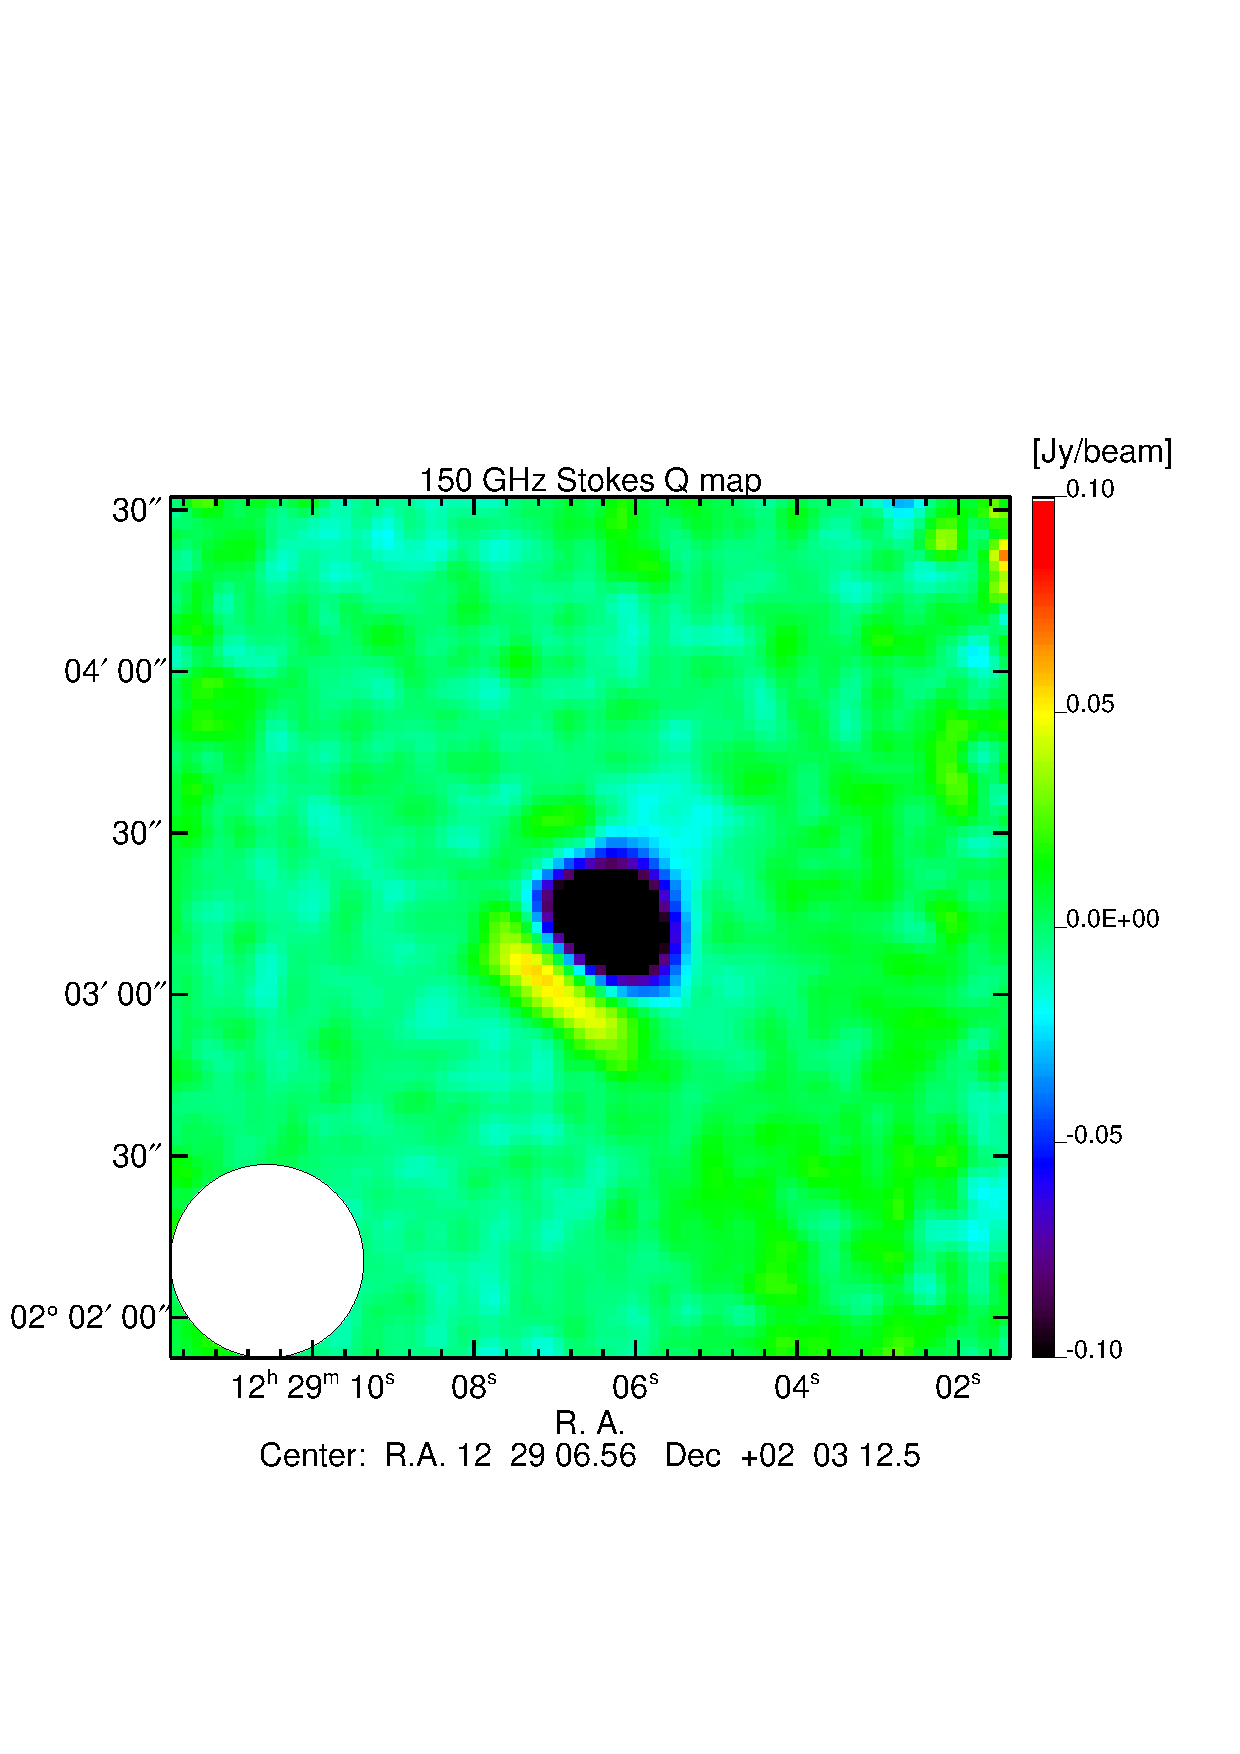
\includegraphics[%
      width=0.25\linewidth,keepaspectratio]{figures/3C273_Q_map_2mm.pdf}
        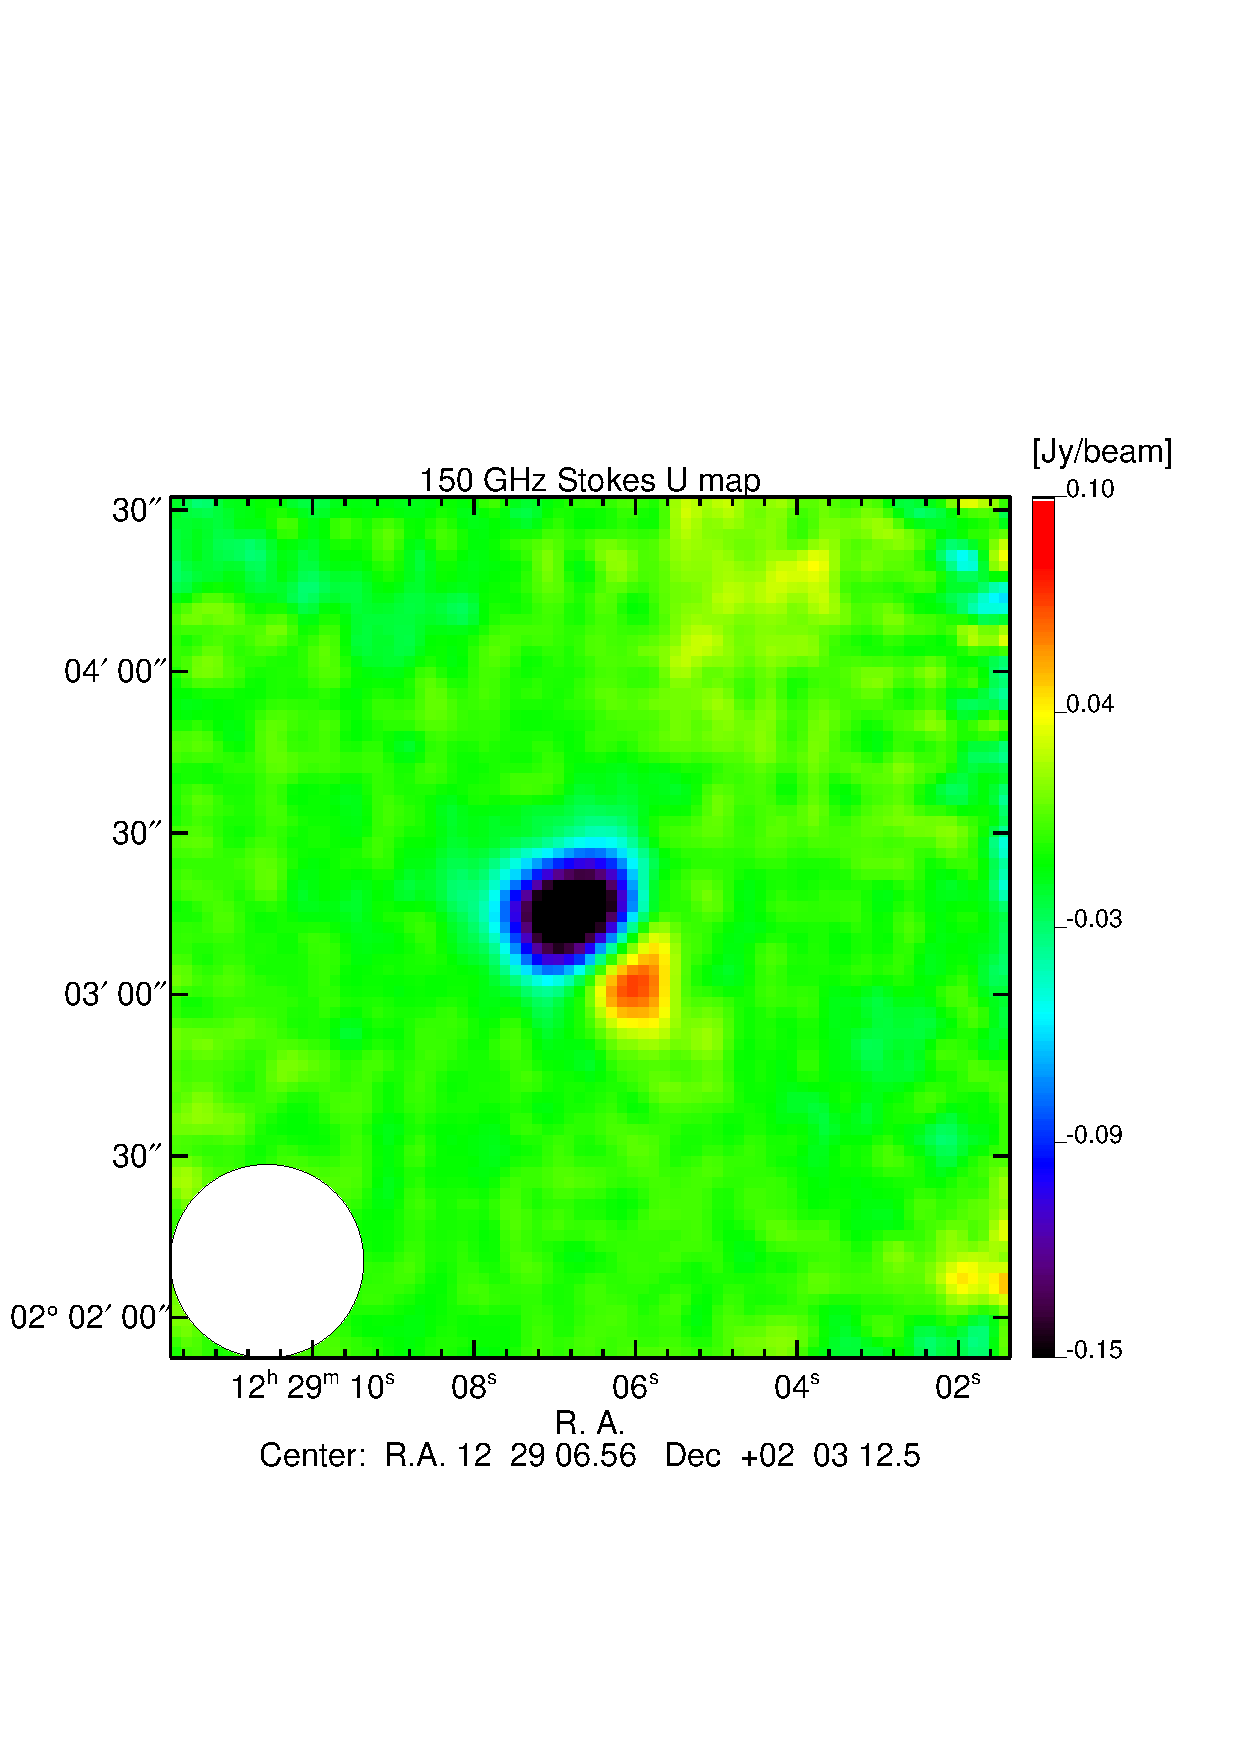
\includegraphics[%
      width=0.25\linewidth,keepaspectratio]{figures/3C273_U_map_2mm.pdf}
       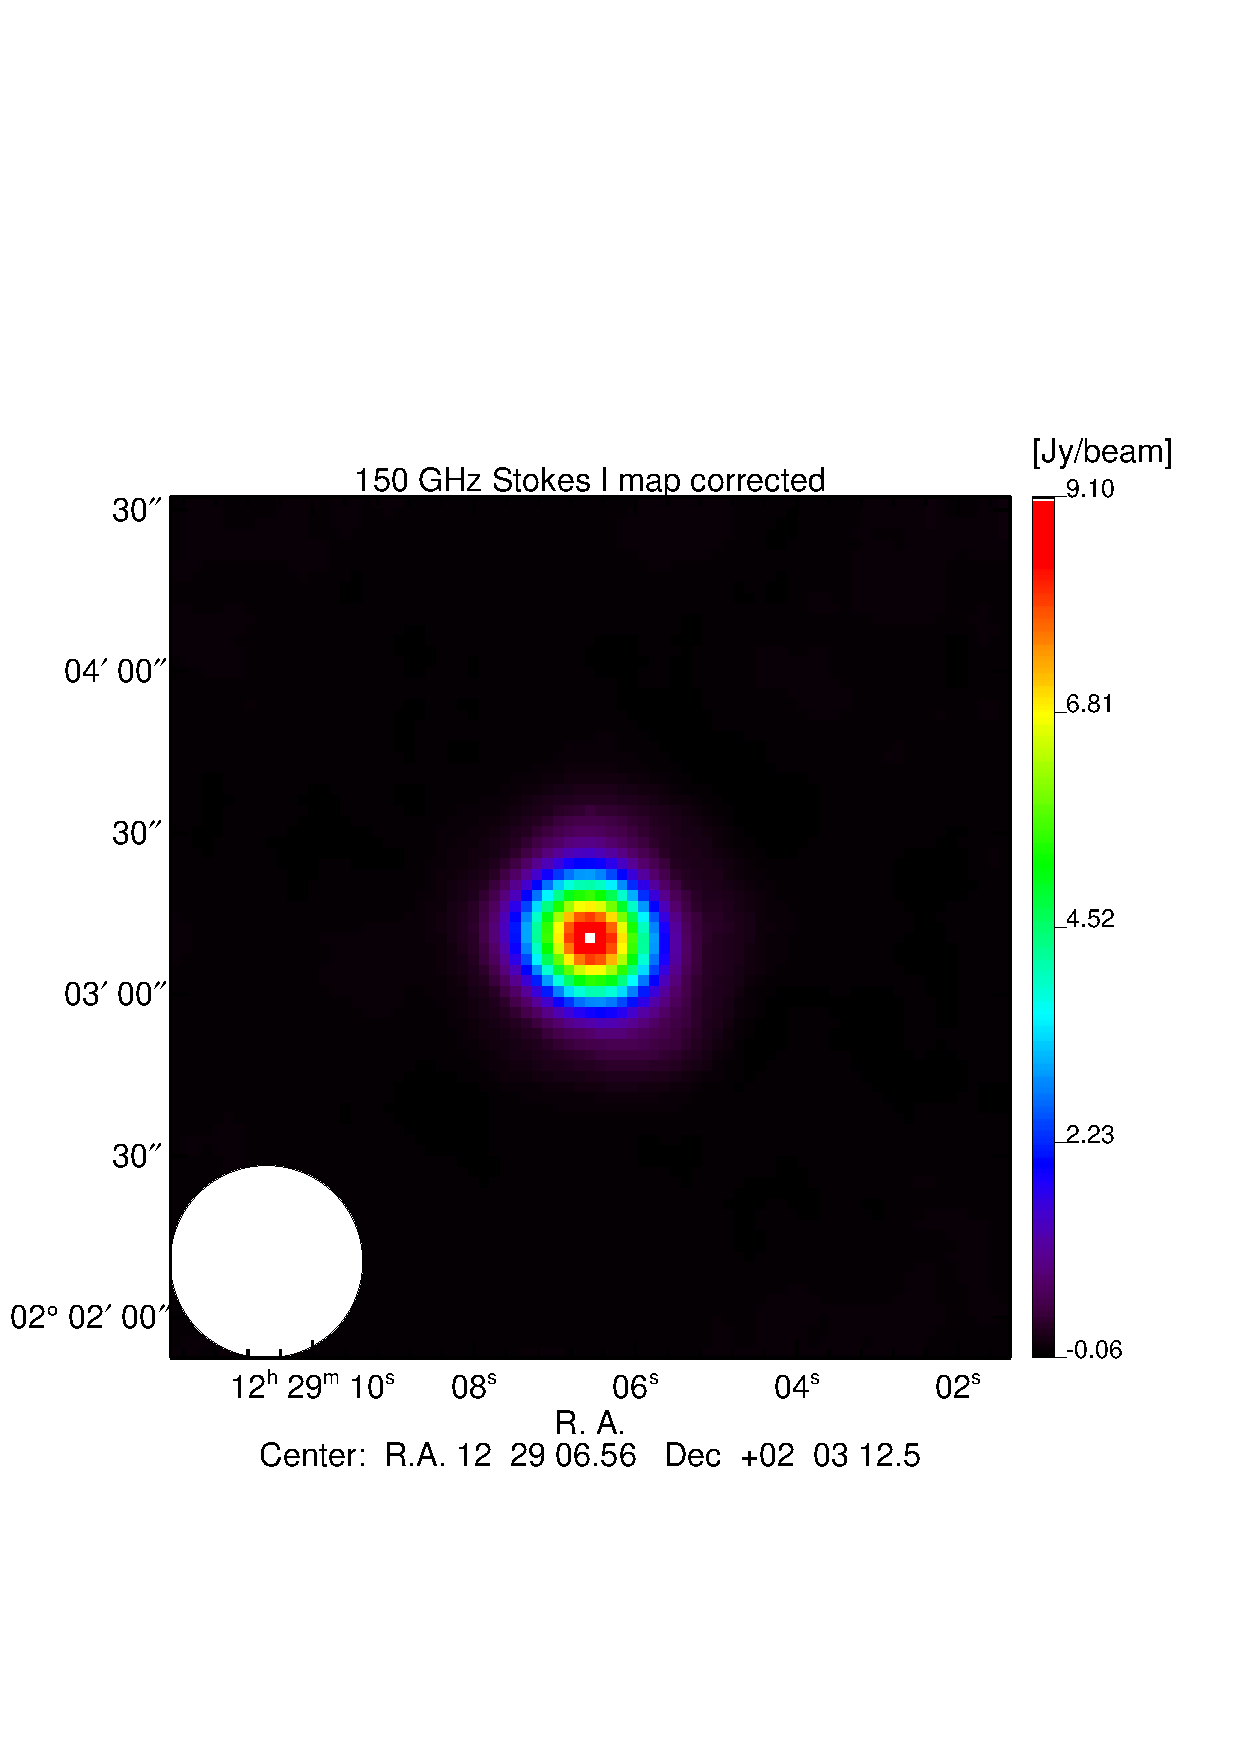
\includegraphics[%
      width=0.25\linewidth,keepaspectratio]{figures/3C273_I_map_2mm_corr.pdf}  
   \includegraphics[%
      width=0.25\linewidth,keepaspectratio]{figures/3C273_Q_map_2mm_corr.pdf}
    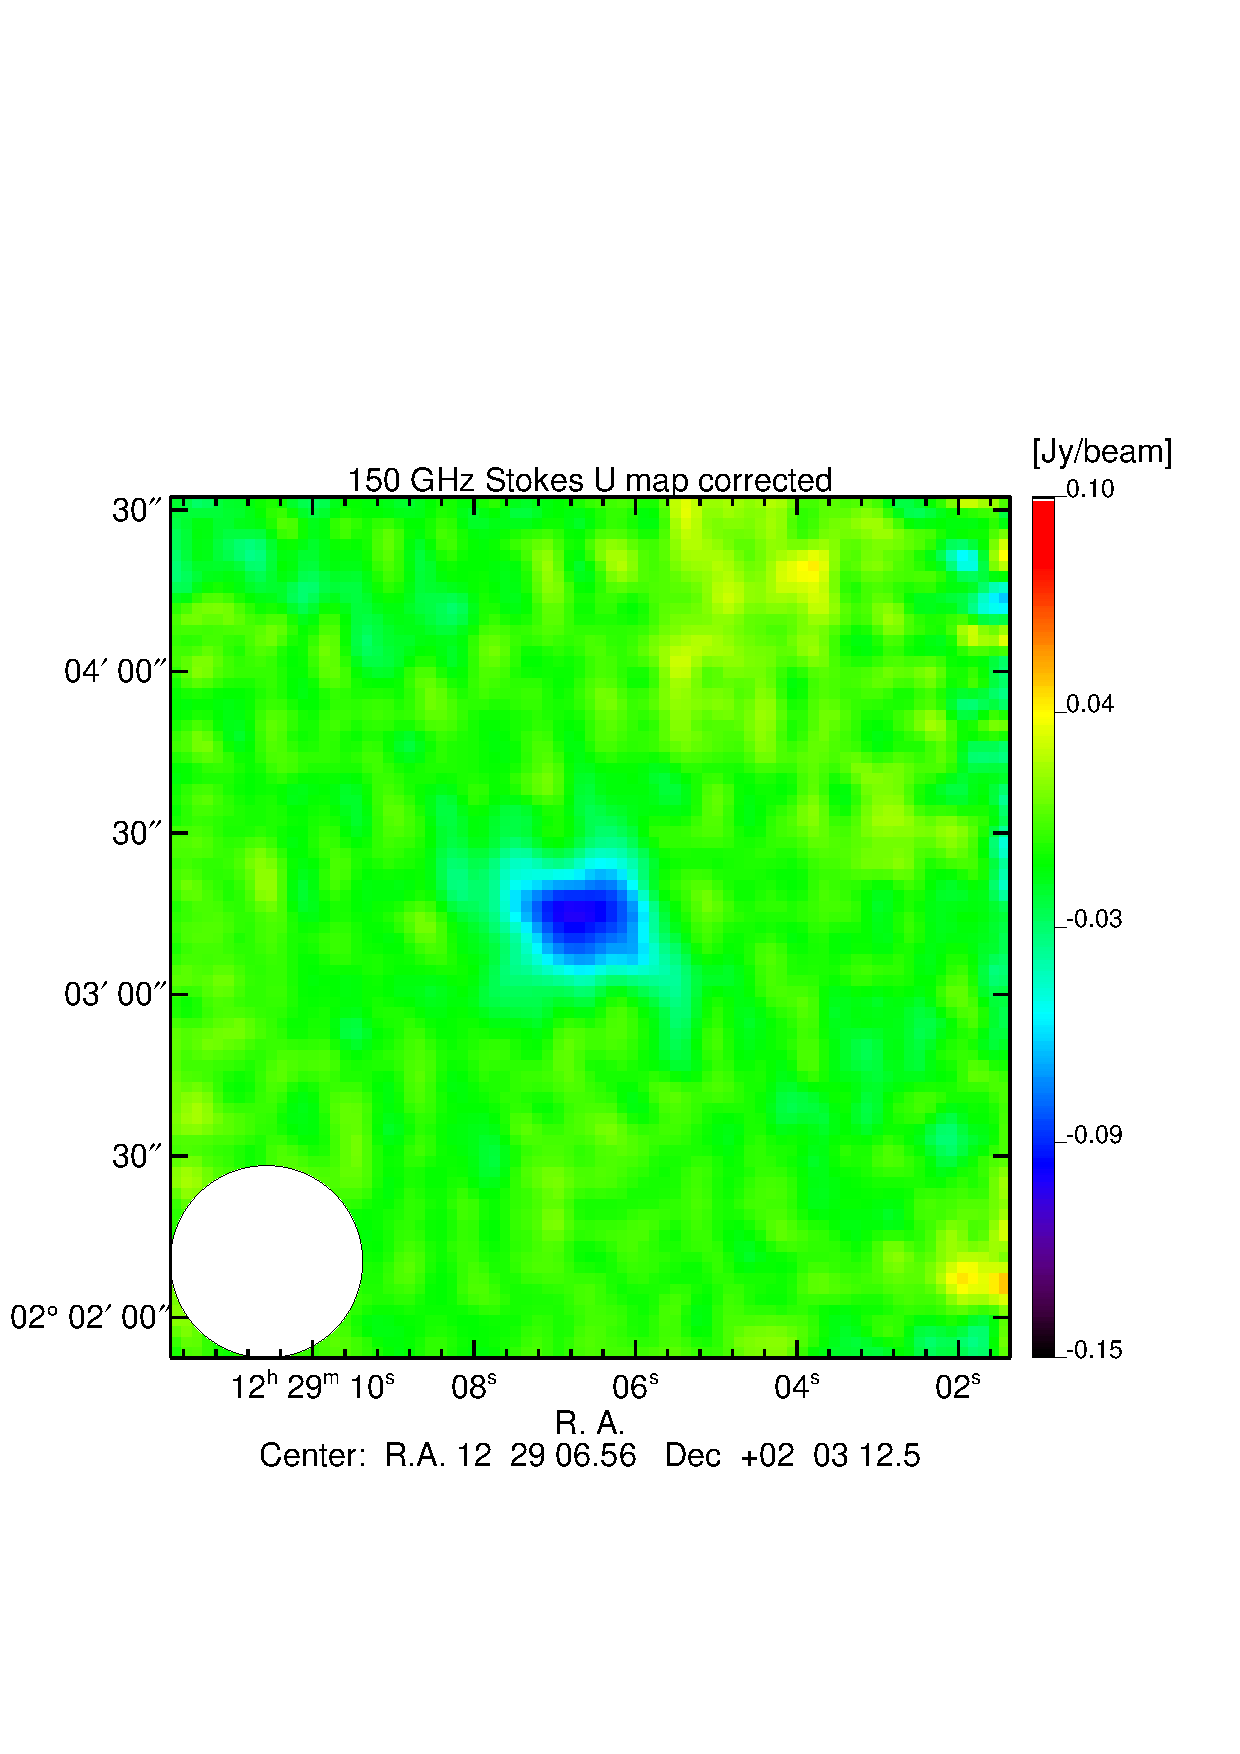
\includegraphics[%
      width=0.25\linewidth,keepaspectratio]{figures/3C273_U_map_2mm_corr.pdf}
      \caption{{\bf Top}: $I$, $Q$, $U$ maps of the quasar 3C 273 observed at 150 GHz
      before correction for the leakage effect. {\bf Bottom}: $I$, $Q$, $U$ maps after correction. The polarization angle and degree are reported in the table \ref{tab:table_quasar}.}
    \label{3c273_ex}
  \end{center}
\end{figure*}


%\begin{figure*}[h]
  %\begin{center}
  %\includegraphics[%
    %  width=0.33\linewidth,keepaspectratio]{figures/3C286_radec_corrected_I_1mm.pdf}
   % \includegraphics[%
    %  width=0.33\linewidth,keepaspectratio]{figures/3C286_radec_corrected_Q_1mm.pdf}
      %  \includegraphics[%
     % width=0.33\linewidth,keepaspectratio]{figures/3C286_radec_corrected_U_1mm.pdf}
     %  \includegraphics[%
    %  width=0.33\linewidth,keepaspectratio]{figures/3C286_radec_corrected_I_2mm.pdf}
  % \includegraphics[%
   %   width=0.33\linewidth,keepaspectratio]{figures/3C286_radec_corrected_Q_2mm.pdf}
   % \includegraphics[%
    %  width=0.33\linewidth,keepaspectratio]{figures/3C286_radec_corrected_U_2mm.pdf}
    %  \caption{Leakage corrected Stokes $I$, $Q$, $U$ maps of the quasar 3C 286 observed at 260 (top) and 150 (bottom) GHz. The polarization angle and degree are reported in the table \ref{tab:table_quasar}.}
   % \label{3c286_maps}
 % \end{center}
%\end{figure*}
\section{Validation of the quality of the \nika\ polarization reconstruction on quasars} \label{polcalibration}
%During the polarization campaign on February the calibration procedure used was
%the same discussed in section \ref{sec:pipeline}, the \emph{skydip} has been
%performed with the operating rotating HWP and the polarization pipeline has been
%used in order to have the TOI intensity Stokes vector $I$
\subsection{Quasar selection and previous observations}
During the \nika\ February 2015 {\nico technical} campaign we have observed a
selection of quasars to validate the quality of the reconstruction of the
polarization signal with the \nika\ camera. We have considered both bright and
highly polarized quasars. As shown in Table~\ref{tab:table_quasar} the selected
targets were 3C279, 3C273, 3C286, 3C345, 1749+096, 0851+202, 0923+392 and
0415+379. We list in the following the main physical characteristics and
polarization properties of the most commonly observed quasars at mm wavelength;
3C286, 3C279 and 3C273.

\subsubsection*{3C 286}
3C 286 is a compact steep-spectrum quasar at redshift z = 0.846.  The stability
of this quasar in intensity and polarization in a large frequency range and the
slow wavelength dependence {\nico make} it a primary calibrator for polarization
measurements. At centimeter wavelengths, where 3C 286 is commonly used as a
primary polarization calibrator, observations show that the 3C286 polarization
angle (PA) has been stable for decades \citep{perley&butler}. At millimeter
wavelengths the {\it XPOl} polarimeter \citep{thum2008} has monitored 3C286 from
2006 to 2012 \citep{xpol}. As presented in Table~\ref{tab:tab_quasar} {\it XPOL}
observations show that 3C 286 is highly polarized, up to 14 \%, with PA
increasing slowly with frequency. These results have been confirmed by
observations at 1.3 mm with the CARMA polarimeter \citep{carma} in May 2015 (see
Table~\ref{tab:tab_quasar}).

%XPOl found a polarization angle $\alpha_{\rm Sky}$ = [37.3 $\pm$ 0.8]$^\circ$ and  $\alpha_{\rm Sky}$ = [33.1$\pm$5.7]$^\circ$, a polarization degree $p$= [13.5 $\pm$ 0.3] $\%$ and $p$ = [14.4$\pm$1.8] $\%$ at 86 and 229 GHz, respectively \citep{xpol}. Recent observation of 3C286 at 1.3 mm done by CARMA polarimeter \citep{carma} reports a polarization angle $\alpha_{\rm Sky}$ = [39.2$\pm$1]$^\circ$. 

%The agreement of the {\it NIKA} results with other millimeter experiments show the good performance of this new polarimeter in polarized light detection. 

\subsubsection*{3C 279}
The blazar 3C 279 is one of the brightest and {\nico best} monitored
flat-spectrum quasars. It was the first object to exhibit apparent superluminal
motion. The source of its strong radio to $\gamma$-ray emission is a
relativistic jet of material ejected from nearby the black hole in its centre
\citep{apex3c279}.  3C279 is a variable source but strongly polarized up to 11
\%.  We present in Table~\ref{tab:tab_quasar} results in terms of degree of
polarization and PA from recent observations of 3C279 by the SHARP polarimeter
\citep{sharp3c279}. These observations were performed in March 2014 at 350
$\mu$m, and at 3.5, 7, 13 mm.

\subsubsection*{3C273}
3C 273, the first quasar ever to be identified, is located in the constellation
of Virgo at a redshift z = 0.158 \citep{3c273madsen}. 3C 273 is the brightest
and hence one of the best monitored Active Galactic Nuclei (AGN). From radio to
millimeter wavelengths flares from the relativistic jet dominate the variability
of 3C 273 \citep{Abdo2010}. 3C 273 shows relatively low polarization, around 3-4
\% (see Table~\ref{tab:tab_quasar}), at mm wavelengths.
%The calibration factor includes the correction for the reduced flux received by
%the LEKIDs due to the warm wire-grid. The calibration uncertainty for point
%sources on the final data is estimated to be 15 \% for the 1.25 mm channel and
%10 \% for 2.05 mm channel, a list of main error sources is detailed in
%citep{catalano2014}. The FWHM of the beam are 13.5 and 18.4 arcsec at 260 GHz
%and 150 GHz.

\subsection{Leakage correction}
The quasar observations presented above can be used to cross check the validity
of the leakage correction presented in~\ref{sec:polleak}. The top row of
Figure~\ref{3c273_ex} shows the \nika\ Stokes $I$, $Q$ and $U$ maps at 2 mm of
the quasar 3C273 before leakage correction. We {\nico **} clearly {\nico see} in
the $Q$ and $U$ maps a dipolar structure similar to the one observed {\nico on} the
Uranus maps. The bottom row of the figure presents the leakage corrected maps,
which show no residual dipolar structure but slightly increased noise
contribution.

 %A similar behaviour is found for the other quasars. For illustration we present in Figure~\ref{3c286_maps} leakage corrected Stokes $I$, $Q$ and $U$ maps of the quasar 3C286 at 1.25 (top) and 2 mm (bottom). We observe that even for such a faint quasar (particularly at 1.25 mm) the leakage correction can be applied without degrading significantly the signal-to-noise in the final polarization maps.  
\subsection{Polarization reconstruction accuracy}
Table~\ref{tab:table_quasar} {\nico presents} the Stokes $I$, $Q$, and $U$
fluxes measured by \nika\ at 1.25 and 2.05 mm for the selected quasars. The
fluxes have been measured using a simple aperture photometry procedure. The
reported uncertainties account for inhomogeneities as well as for correlated
noise in the maps \citep[see][for details]{adam2014}. The Stokes $I$, $Q$ and
$U$ fluxes are combined to compute the degree of polarization, $p = \sqrt{(Q^2 +
  U^2)}/I$ and the polarization angle $\chi = \frac{1}{2} \arctan\frac{U}{Q}$
{\nico defined between 0 and $\pi$ **}. Uncertainties in the degree and
  angle of polarization are computed assuming Gaussian errors in the Stokes $I$,
  $Q$ and $U$ fluxes. In the case of the polarization angle a systematic
  uncertainty of 1.8$^\circ$ is added to account for uncertainties in the
  position of the zero of the HWP.

We start by comparing the \nika\ results on the degree and angle of polarization
of 3C286, which is considered a polarization calibrator at mm wavelengths, to
those of the CARMA \citep{carma} and XPOL \citep{xpol} experiments presented in
Table~\ref{tab:tab_quasar}. The 1.3 mm XPOL and CARMA data are consistent within
error bars with the 1.25 mm \nika\ data, confirming that 3C286 is highly
polarized. At 2.05 mm (\nika\ data) and 3 mm (XPOL data) the measured degree and
angle of polarization are consistent with the 1 mm data. Similar results are
found by comparing the \nika\ data for 3C279 with those of SHARP
\citep{sharp3c279} at 350 $\mu$m, and at 3.5, 7, 13 mm.

For the other quasars the comparison of the \nika\ results with other
experiments is much more complex due to either lack of reliable data in the
literature or strong intrinsic variability.  To overcome this problem
measurements with XPOL at the IRAM 30 m telescope were planed an performed in
the same period {\nico as} the \nika\ observations. A summary of the results of
this campaign are given in Table~\ref{tab:tab_quasar}. For 3C273 the \nika\ and
XPOL results are consistent in terms of polarization degree when comparing 1.3
and 1.25 mm, and 2 and 3 mm.  The 1.3, 2 and 3 mm data are consistent in {\nico
  terms} of polarization angle. However the 1.25 mm \nika\ data present a
significantly different (in terms of uncertainties) polarization angle, which
may be induced by residual leakage contamination. For the other quasars although
the polarization degree is relatively consistent between \nika\ and XPOL
measurements, the polarization angle are clearly inconsistent. To date no
explanation has been found for this. {\nico je pense qu'il faut reprendre un peu
  ces deux phrases, on ne peut pas dire que c'est peut-\^etre du residual leakage
  sans chiffrer et dire la phrase suivante qu'on ne sait pas d'o\`u \c ca
  vient. Est ce que \c ca peut-\^etre expliqu\'e par la variabilit\'e des quasars, pas que
  l'intensit\'e mais aussi la direction de polarisation ?}
%The polarization degree $p$ is defined by 
%\begin{equation}
%p = \sqrt{(Q^2 + U^2)}/I
%\end{equation}
%with uncertainty:
%\begin{equation}
%\sigma p = p^{\rm -1} \sqrt{dQ^2Q^2 + dU^2U^2}
%\end{equation}
%and the polarization angle $\alpha_{\rm Sky}$
%\begin{equation}
%\alpha_{\rm Sky} = \frac{1}{2} \arctan\frac{U}{Q} ,  0 < \alpha_{\rm Sky} < \pi
%\end{equation}
%with statistical uncertainty:
%\begin{equation}
%\sigma\alpha_{\rm Sky}^{\rm stat} = \frac{1}{2}\{(Q^2+U^2)\sqrt{Q^2dU^2 + U^2dQ^2}\}^{\rm -1}%end{equation}
%The polarization angle is directly measured on the Sky considering the HWP zero defined with respect to the Nasmyth coordinates reference frame. A synchronized acquisition software provides the rotation angles of the HWP taken into account in the data analysis. As discussed above our precision in the determination of the HWP zero is 1.8$^\circ$, this is considered a systematic error in polarization angle measurements.
%In the following sections we discuss the {\it NIKA} results comparing with previous observations. 
\subsection{Photometric accuracy}
The measurement of relatively stable quasars as 3C286 and 3C273 allows us also
to cross check the quality of the \nika\ photometry in
intensity. Figure~\ref{sed} {\nico presents} the spectral energy density (SED)
as a function of frequency in GHz for 3C286 (left) and 3C273 right. The
\nika\ intensity flux and uncertainties at 1.25 and 2.05 mm are represented in
blue.  Results from other experiments including {\it XPOL} \citep{thum2008},
PLANCK \citep{planckcatalogue} and ALMA \citep{almacalib} are presented in
black. We observe that the \nika\ data are consistent within error bars with the
other experiment results. We find that the 3C286 data are consistent with a
synchrotron spectrum in the form of a power law, $\propto$ $\nu^{\rm \beta}$,
with spectral index $\beta$ $\simeq$ -1.007 $\pm$ 0.033 (dashed red line).  To
explain the 3C273 data we {\nico considered} two power laws with spectral {\nico
  indices} $\beta_1$ $\simeq$ -0.29$\pm$0.05 and $\beta_2$ $\simeq$
-0.85$\pm$0.06 (dashed red line).
\begin{figure*}
 \begin{center}
  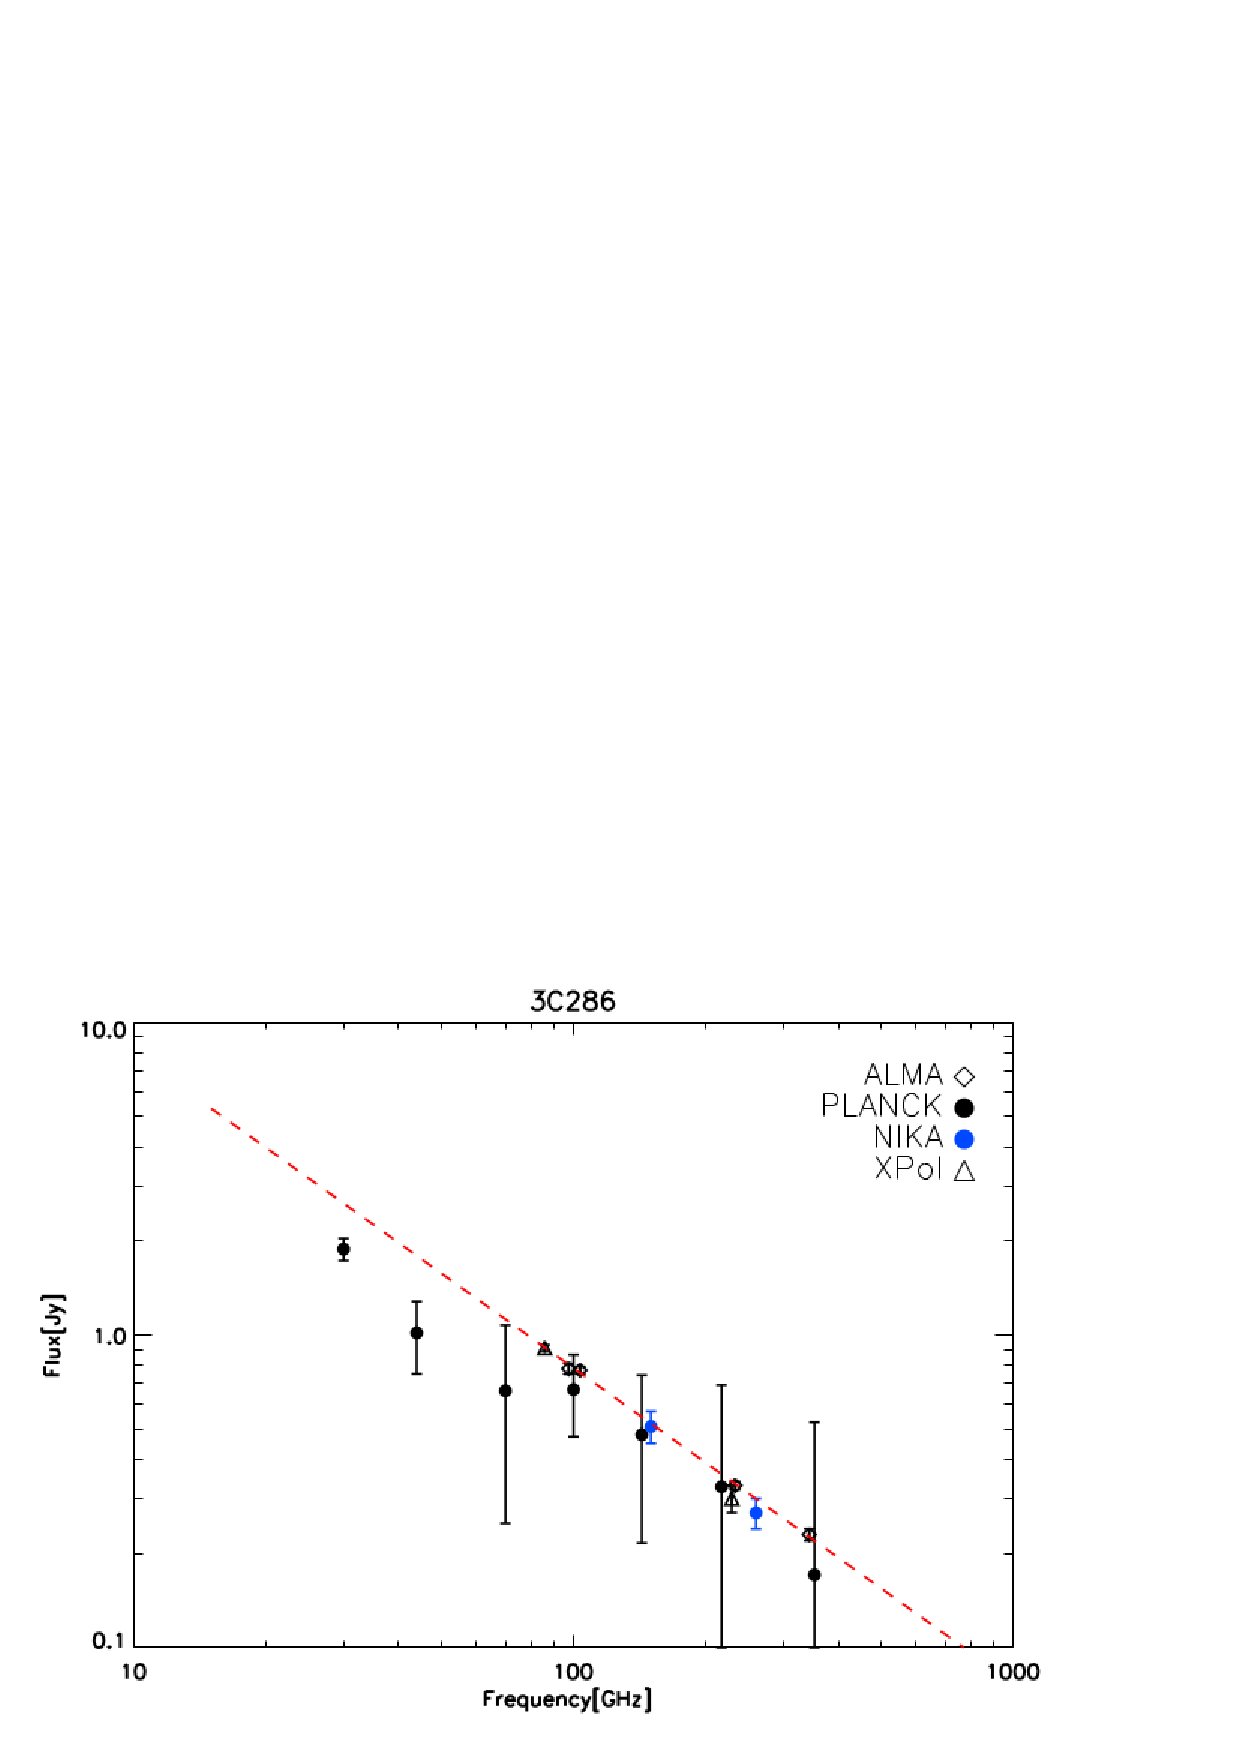
\includegraphics[%
  width=0.4\linewidth,keepaspectratio]{figures/ALMA_PLANCK_sed2_3C286.pdf}
  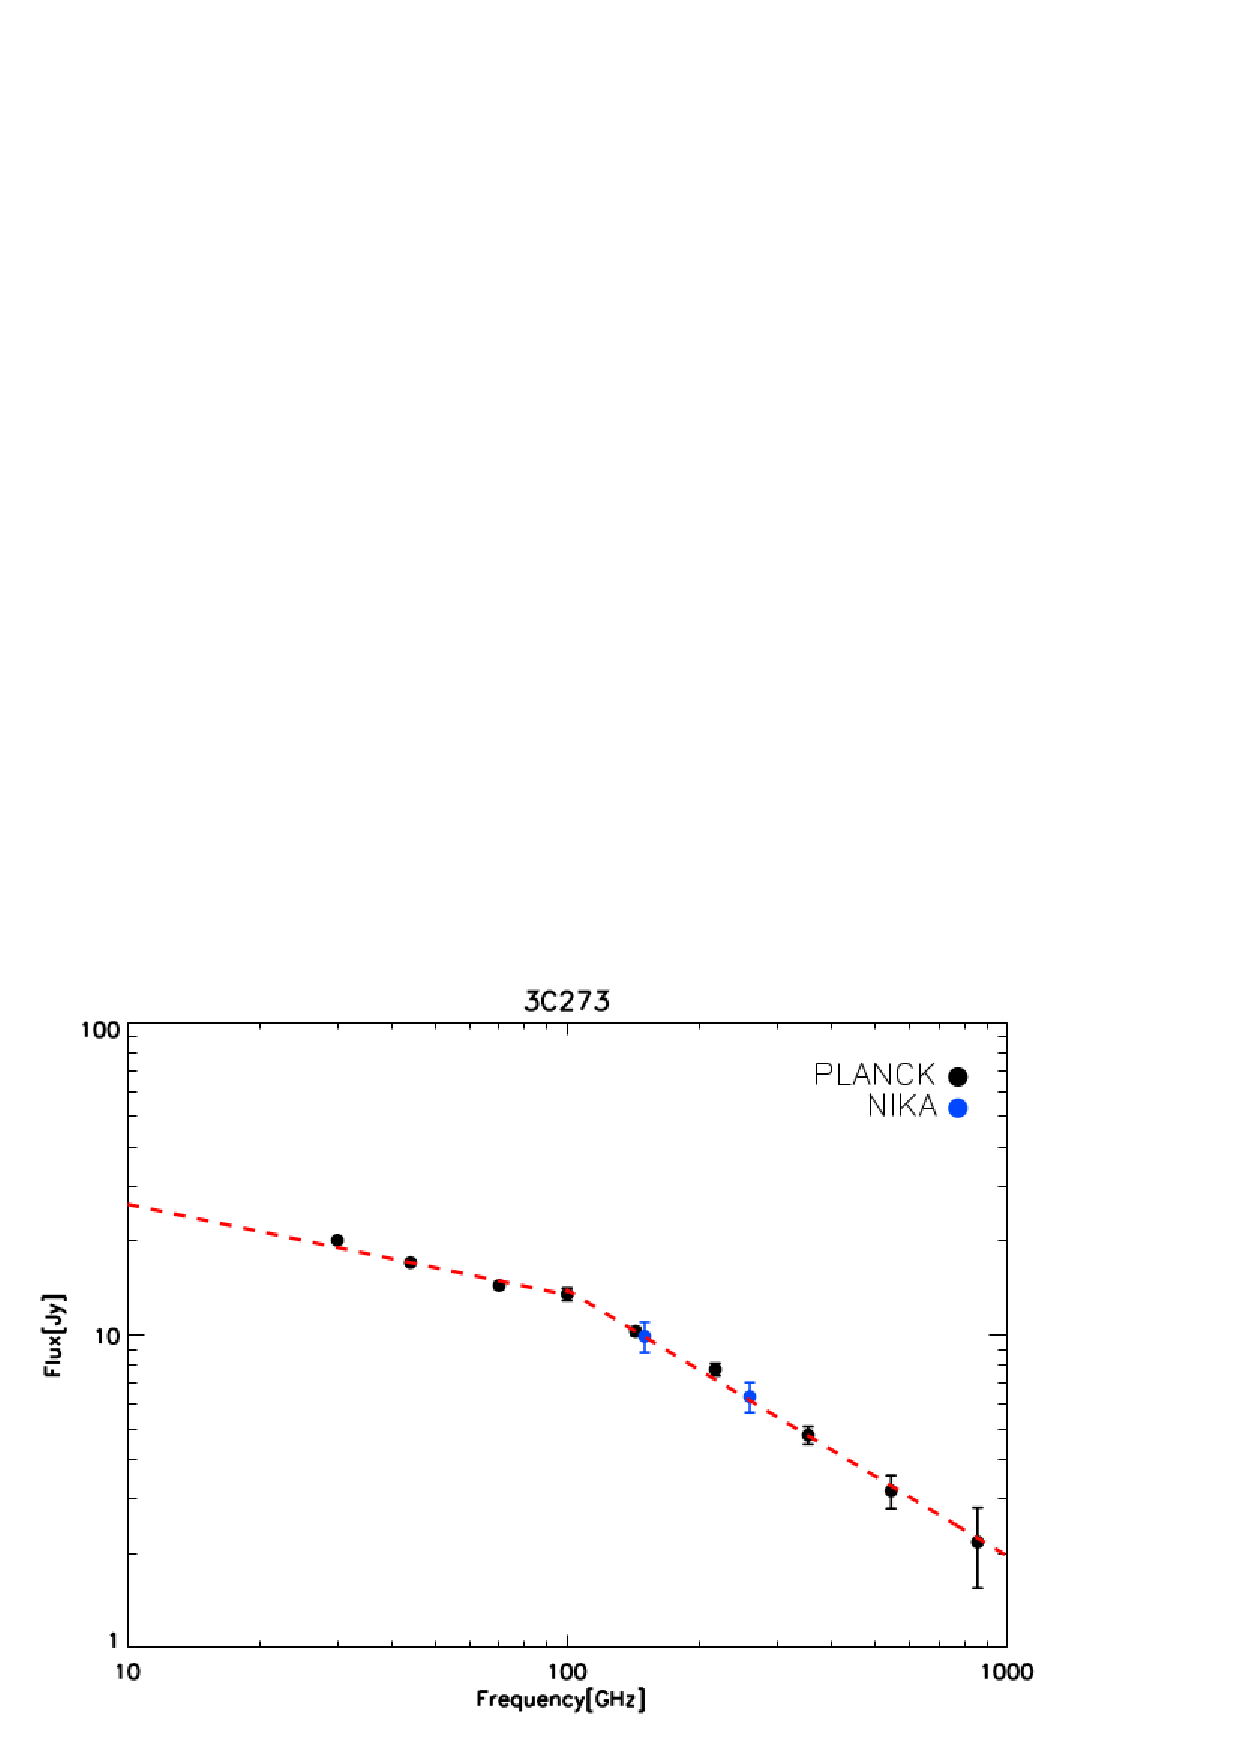
\includegraphics[%
  width=0.4\linewidth,keepaspectratio]{figures/ALMA_PLANCK_sed2_3C273.pdf}
  \caption{ Spectral energy density (SED) for the quasars 3C286 (left) and 3C273 (right). We consider data from PLANCK \citep[black dot, ][]{planckcatalogue}; ALMA \citep[black diamond,][]{almacalib}; XPOl \citep[black triangle,][]{xpol} and \nika\  (blue dot, this paper).  \label{sed}}
 \end{center}
  \end{figure*}
 
%In order to cross check at the opacity correction and photometric calibration we
%compare the results of four quasars (3C 273, 1749+096, 0851+202, 0415+379)
%observed by {\it NIKA} and XPOl experiment \citep{thum2008} during a parallel
%session of observation during the observational campaign on February 2015. In
%the tab. \ref{tab:calib} we can see the consistency of {\it NIKA} results with
%XPOl observations. 
%The calibration error, reported in \citep{catalano2014} is of
%the order of $\sim$ 10 $\%$ and is taken into account in the statistical
%error. The K-correction is $\sim$ 1-2 $\%$ for the synchrotron spectra of
%quasars, so it is negligible respect to the calibration error estimation.

%\begin{table*}
%\begin{center}
%\begin{tabular}{ccccccccc}
%\hline
%\hline
%Source & I flux Xpol 1.25 mm & I flux Xpol 3 mm &  I flux {\it NIKA}  1.25 mm& I flux {\it NIKA}  2.05 mm\\
% & [K] & [K] & [K] & [K]\\
%\hline
%3C273 & 0.614 $\pm$0.002      &  2.304 $\pm$ 0.002  & 0.60$\pm$ 0.09    &  1.35$\pm$0.23\\
%1749+096 & 0.201$\pm$0.001 & 0.558$\pm$0.001     & 0.15$\pm$0.03     &  0.26$\pm$0.06\\
%0851+202 & 0.384$\pm$0.002 & 0.989$\pm$0.001     & 0.31$\pm$0.06     &  0.57$\pm$0.13 \\
%0415+379 & 0.117$\pm$0.002 &  0.343 $\pm$0.001   & 0.122$\pm$0.025 &  0.238$\pm$0.055\\
%\hline
%\end{tabular}
%\end{center}
%\caption{Intensity flux results from the parallel session of observations between XPOl and {\it NIKA}.}
%\label{tab:calib}
%\end{table*}


%The Tab. \ref{tab:calib} show the consistency of {\it NIKA} flux measurements with XPOl results at 1mm.

%To compare with other experiments we choose two of the quasars collection that we had, 3C 273 and 3C 286. In Fig. \ref{sed_3C286} we show the spectral energy density (SED) for the quasar 3C286, which is considered a primary calibrator for polarization experiments too. 

%We plot the results obtained by PLANCK \citep{planckcatalogue}, ALMA \citep{almacalib}, XPOl \citep{xpol} and {\it NIKA} polarization campaign (February 2015).  We observe a synchrotron spectrum with a power law $\propto$ $\nu^{\rm \beta}$ with spectral index  $\beta$ $\simeq$ -1.007 $\pm$ 0.033. The fig. \ref{sed_3C273} presents the PLANCK and NIKA results for the quasar 3C273, the spectrum shows two power laws with spectral index $\beta_1$ $\simeq$ -0.29$\pm$0.05 and $\beta_2$ $\simeq$ -0.85$\pm$0.06. 

%These two figures \ref{sed_3C273}, \ref{sed_3C286} shows the good photometric calibration effectuated and consistency of the {\it NIKA} results.



%\begin{figure}
 %\begin{center}
  %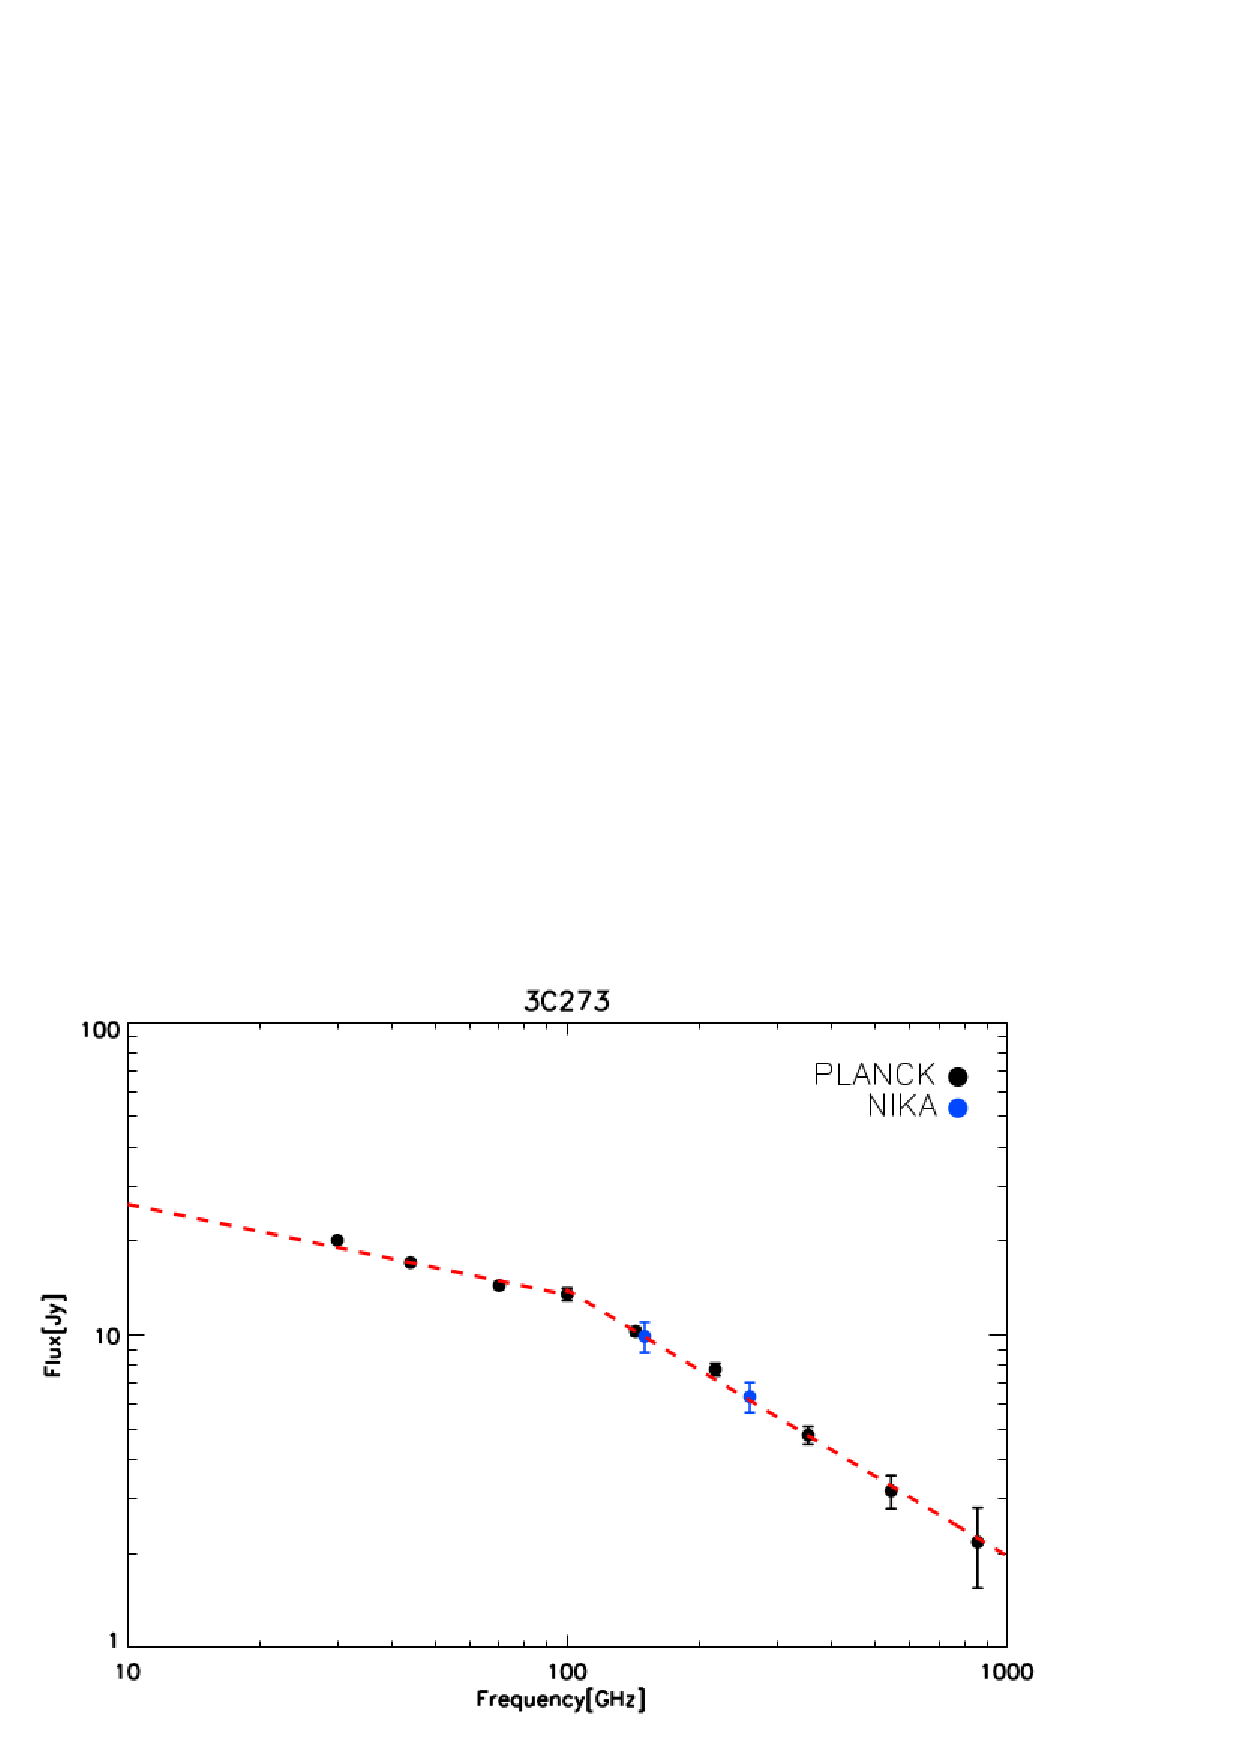
\includegraphics[%
 % width=0.66\linewidth,keepaspectratio]{figures/ALMA_PLANCK_sed2_3C273.pdf}
 % \caption{ 3C 273 spectral energy density (SED) of PLANCK and {\it NIKA} .}
 % \label{sed_3C273}
% \end{center}
 % \end{figure}
  
% Instrumental polarization and results ------------------------------------------------------------------------     

%\section{Polarimetry calibration}\label{polcalib}


%In order to give an example on a polarized source we show the maps obtained for the quasar 3C 273 in Fig. ~ \ref{3c273_ex}. In this figure we show the maps before applying the algorithm of correction (left column) and after (right column); the efficiency of this correction allows us to estimate a more correct polarization degree and angle. Here the quasar is taken as example but a proper discussion on the results obtained in terms of polarization degree and angle is given in the calibration section. 




%\subsubsection{Parallel session {\it NIKA} - XPOl}
%On February 2015 we performed an observational parallel session with XPOl experiment. In this section we will discuss the results obtained by the data analysis from the two experiments. 
%The results of this parallel session of the observations done between {\it NIKA} and XPOl are shown in Tab. \ref{tab:calib_degree}. 

%As Faraday rotation is proportional to $\lambda^2$  \citep{mckee} Faraday rotation measures (RMs) are expected to diminish at high frequencies. The core of the 3C273 shows this trend \citep{Attridge} at 86 GHz and explains the XPOl results. 

%There are some differences and incompatibilities between {\it NIKA} and XPOl data, most of them are likely due to expected trends between the different wavelengths of the instruments. At higher frequencies closer to the base of the jet the magnetic field tends to be more ordered. This can be explain why the polarization degree tends to increase towards higher frequency. 

%The polarization angle is mainly affected by Faraday rotation which changes the angle as proportional $\lambda^2$. It is a weak effect at mm wavelengths, but clearly present in the more active AGNs. This affects more the 3 mm than 2 and 1 mm data. 

%An other effect must also be expected due to changing optical depth with frequency which allows to see different parts of the jet where the magnetic field (and thus the polarization angle) may be different. 

%As Faraday rotation is proportional to $\lambda^2$  \citep{mckee} Faraday rotation measures (RMs) are expected to diminish at high frequencies. The core of the 3C273 shows this trend \citep{Attridge} at 86 GHz and explains the XPOl results. 

%{\it NIKA} polarimeter measures {$\psi$} = (-89.3 $\pm$ 3.2)$^\circ$ and $\psi$ = (-74.1 $\pm$ 3.9)$^\circ$, $p$ = [3.8$\pm$0.4] $\%$ and $p$=[2.0 $\pm$ 0.5] $\%$ at 260 GHz and 150 GHz, respectively. 

%XPOl measures {$\psi$} = (-76.8 $\pm$ 1.6)$^\circ$  and {$\psi$} = (-37.8 $\pm$ 0.9)$^\circ$, $p$ = [3.6$\pm$0.2] $\%$ and $p$ = [1.1$\pm$0.0] $\%$ at 229 GHz and 86 GHz, respectively.

%This is the strongest source that we observed in parallel with XPOl and there is agreement between two experiments in both polarization degree and angle.

%For the quasar 0851+202 there is a clear discrepancy in the angles between instruments for which we do not have an explanation. May be we have to check in the next observations. There is an agreement for both {\it NIKA} wavelengths.

%For the quite variable quasar 1749+096 the {\it NIKA} 1 mm polarization degree is higher than XPOl that observes at 229 GHz.

%The quasar 0415+379 is the weakest source at 1mm and however quite variable. It is too weak for XPOl measurement, we observe however an agreement between the two mm channel of {\it NIKA}.


% Extended sources section --------------------------------	
%OMC-1
 \begin{figure*}
  \begin{center}
  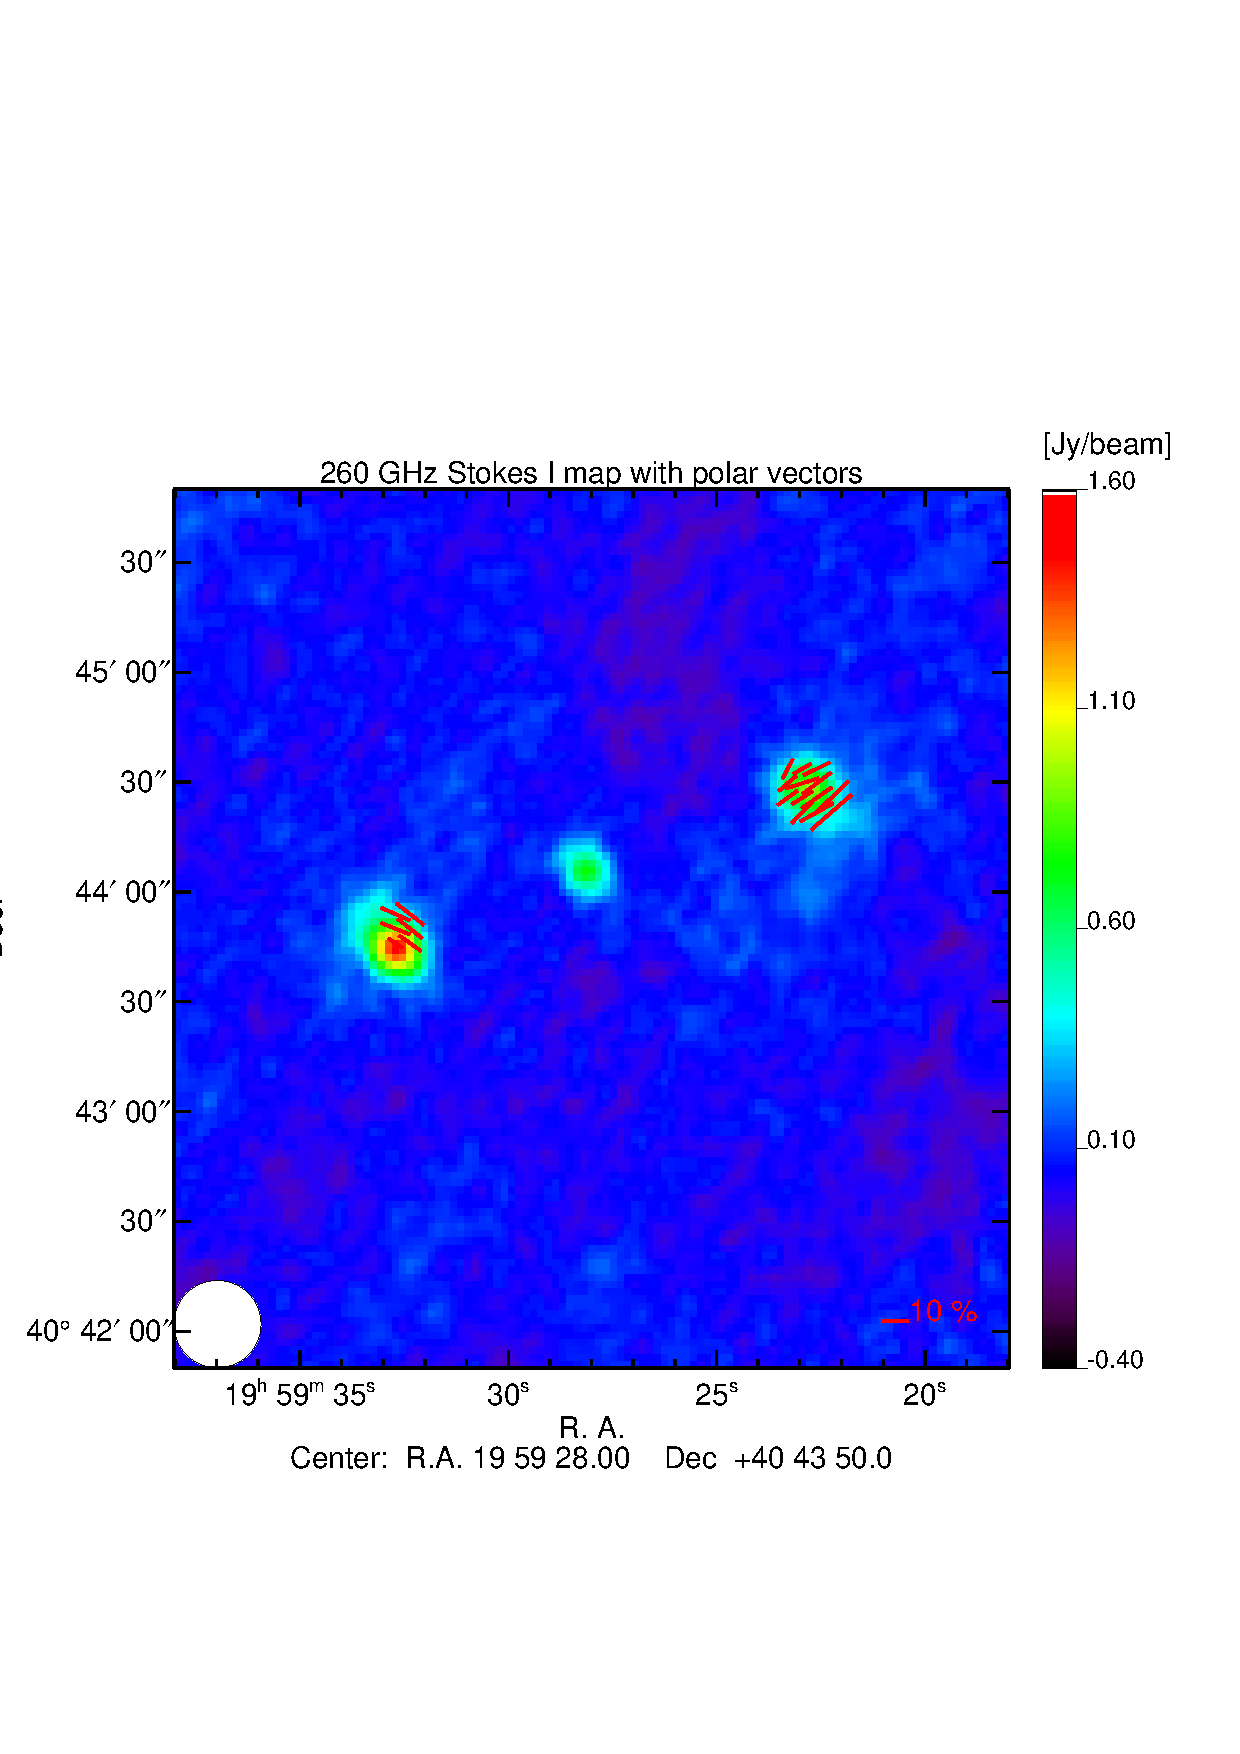
\includegraphics[%
  width=0.33\linewidth,keepaspectratio]{figures/CYGNUSA_I_map.pdf}
   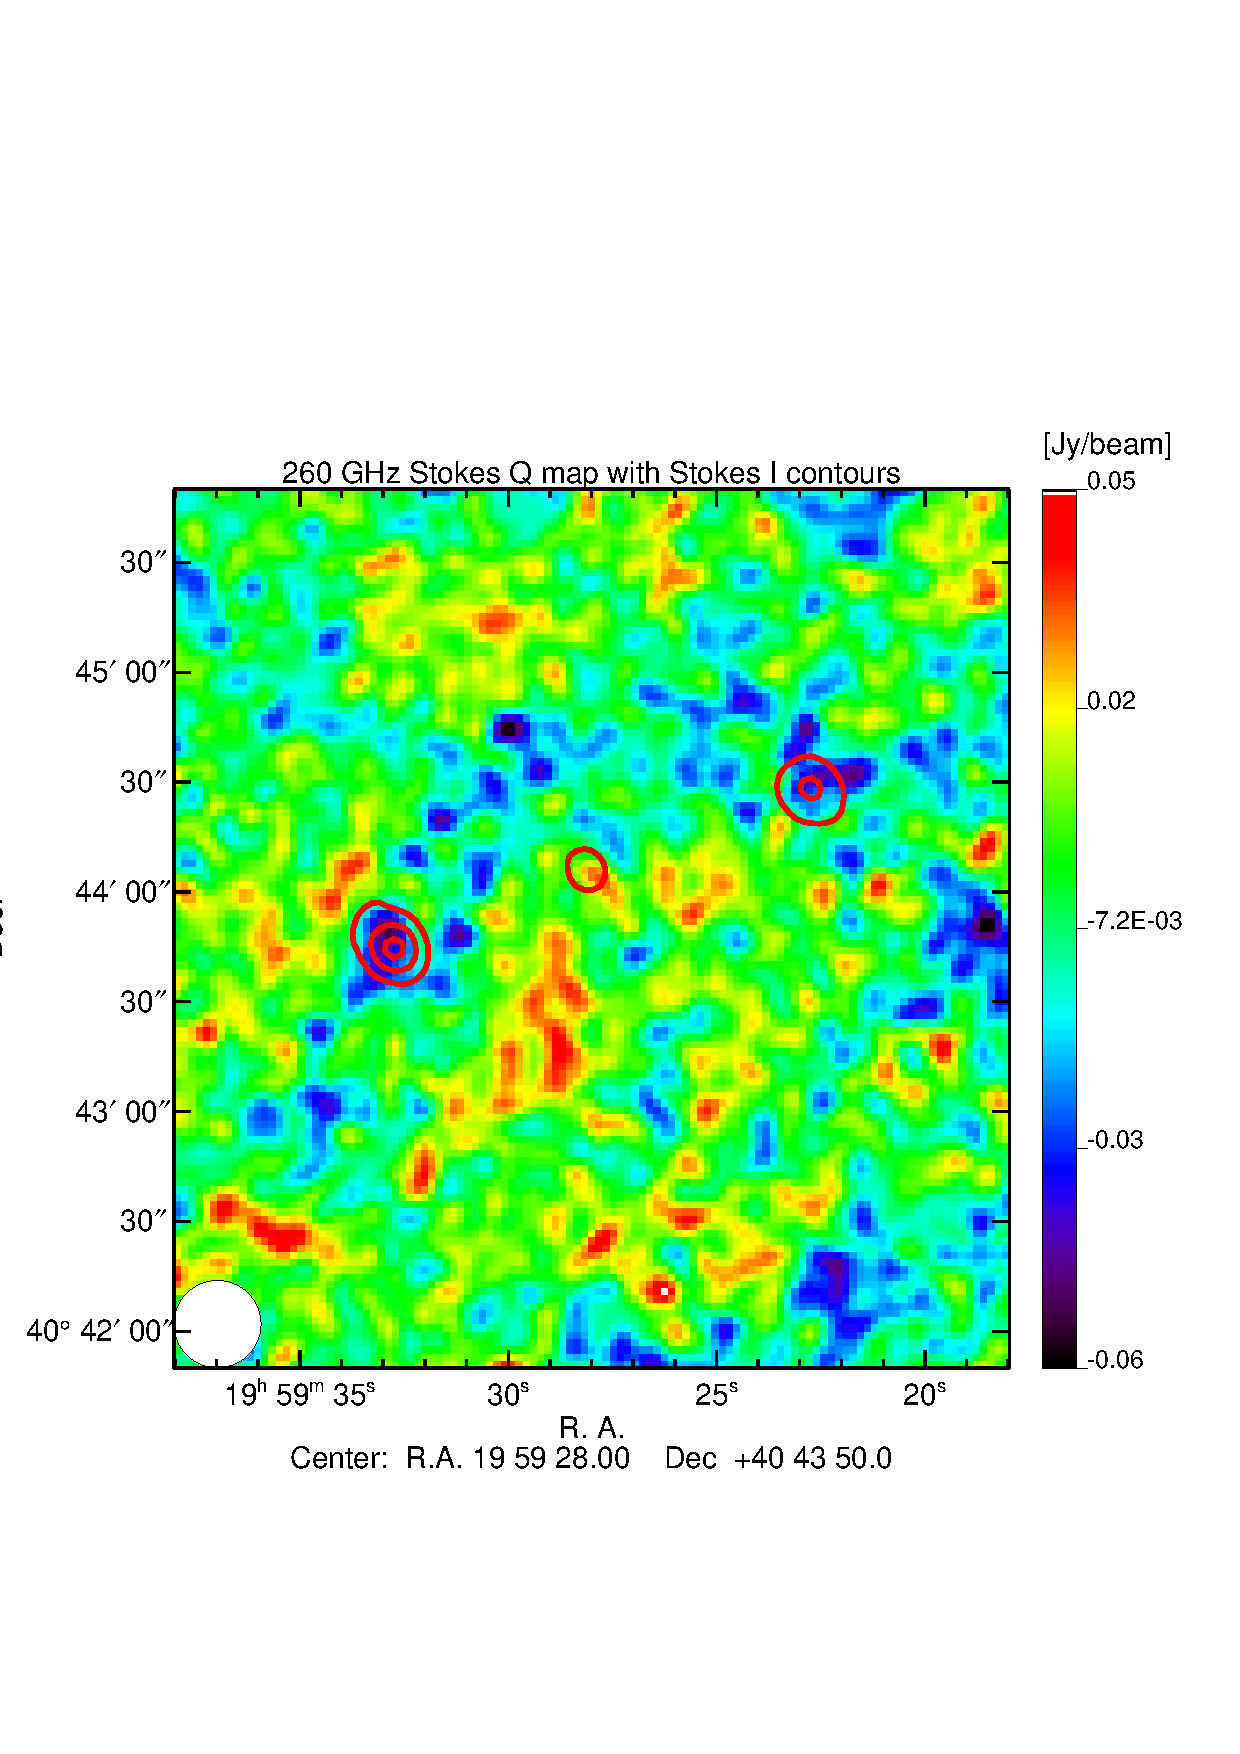
\includegraphics[%
  width=0.33\linewidth,keepaspectratio]{figures/CYGNUSA_Q_map.pdf}
   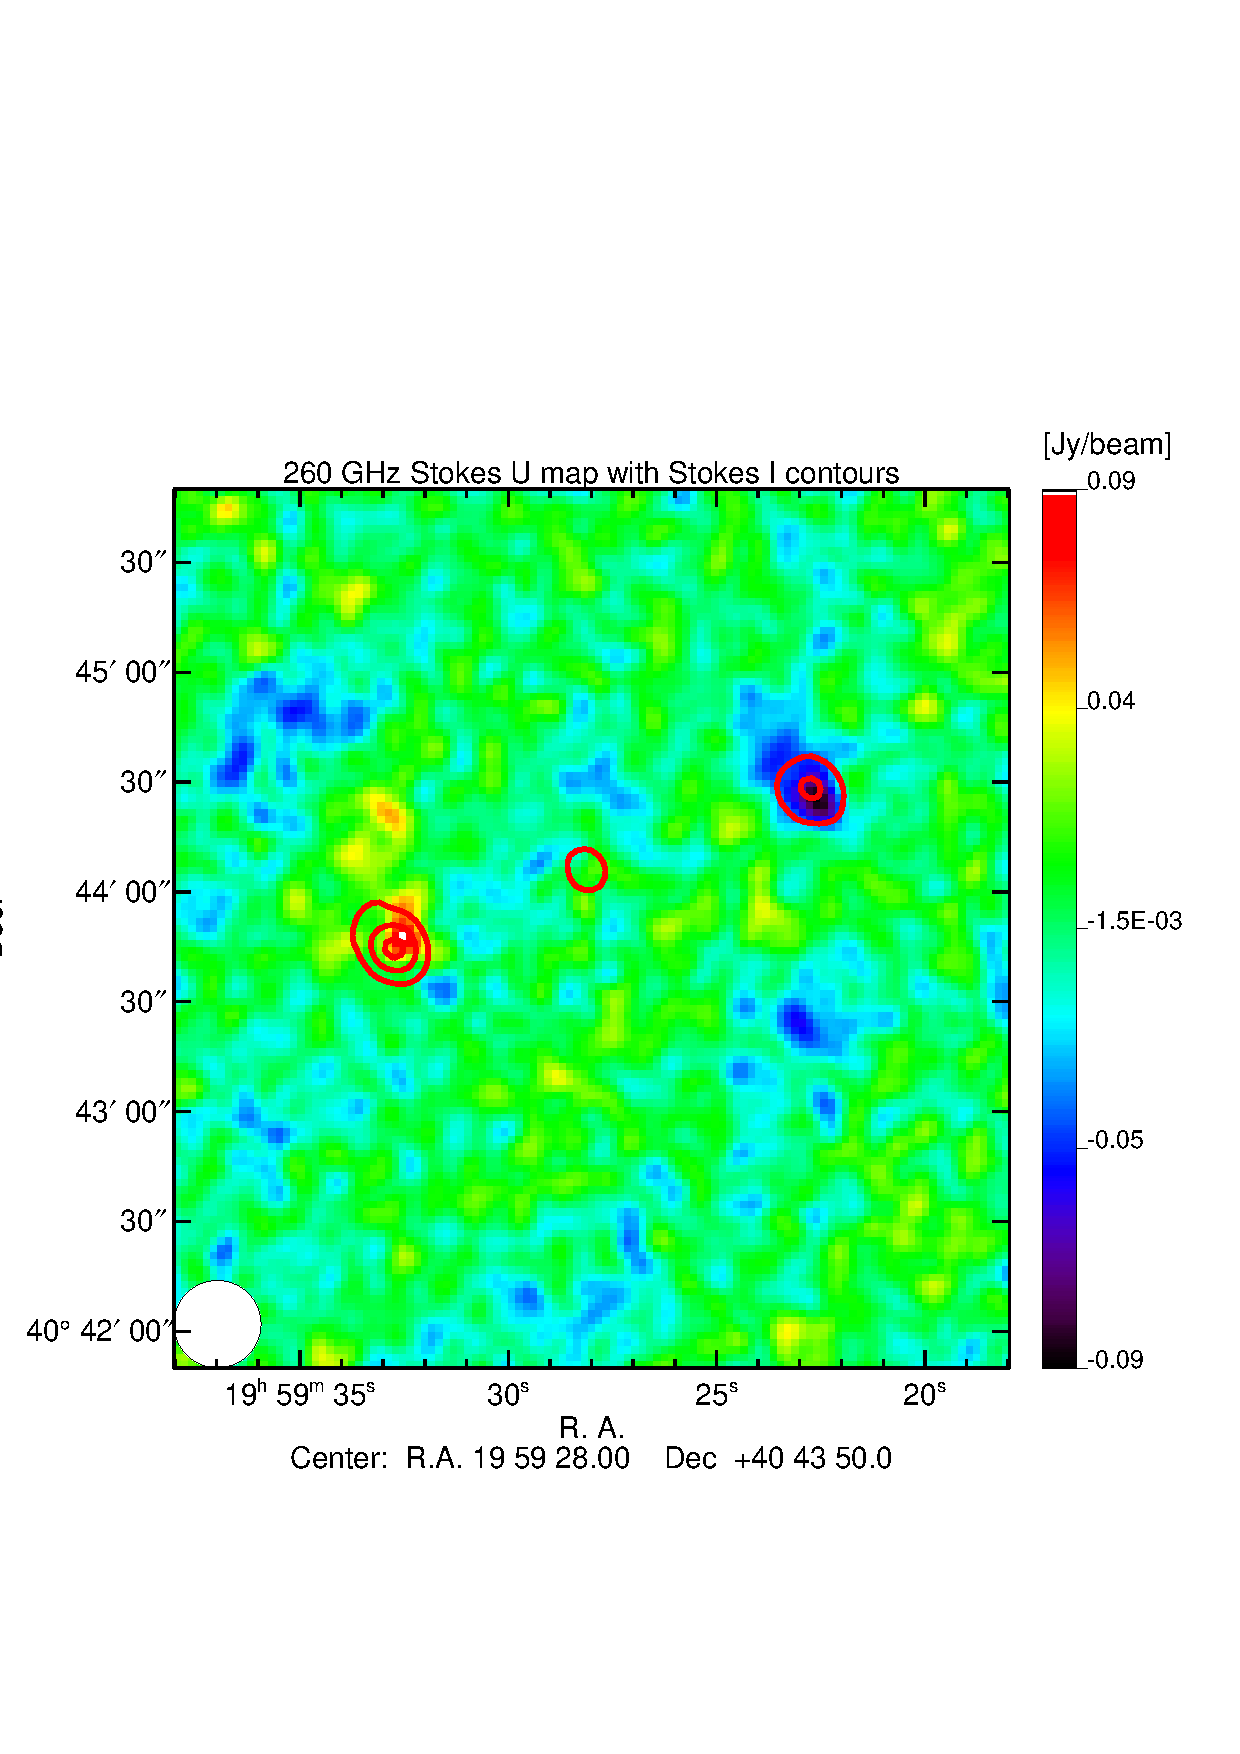
\includegraphics[%
  width=0.33\linewidth,keepaspectratio]{figures/CYGNUSA_U_map.pdf}
   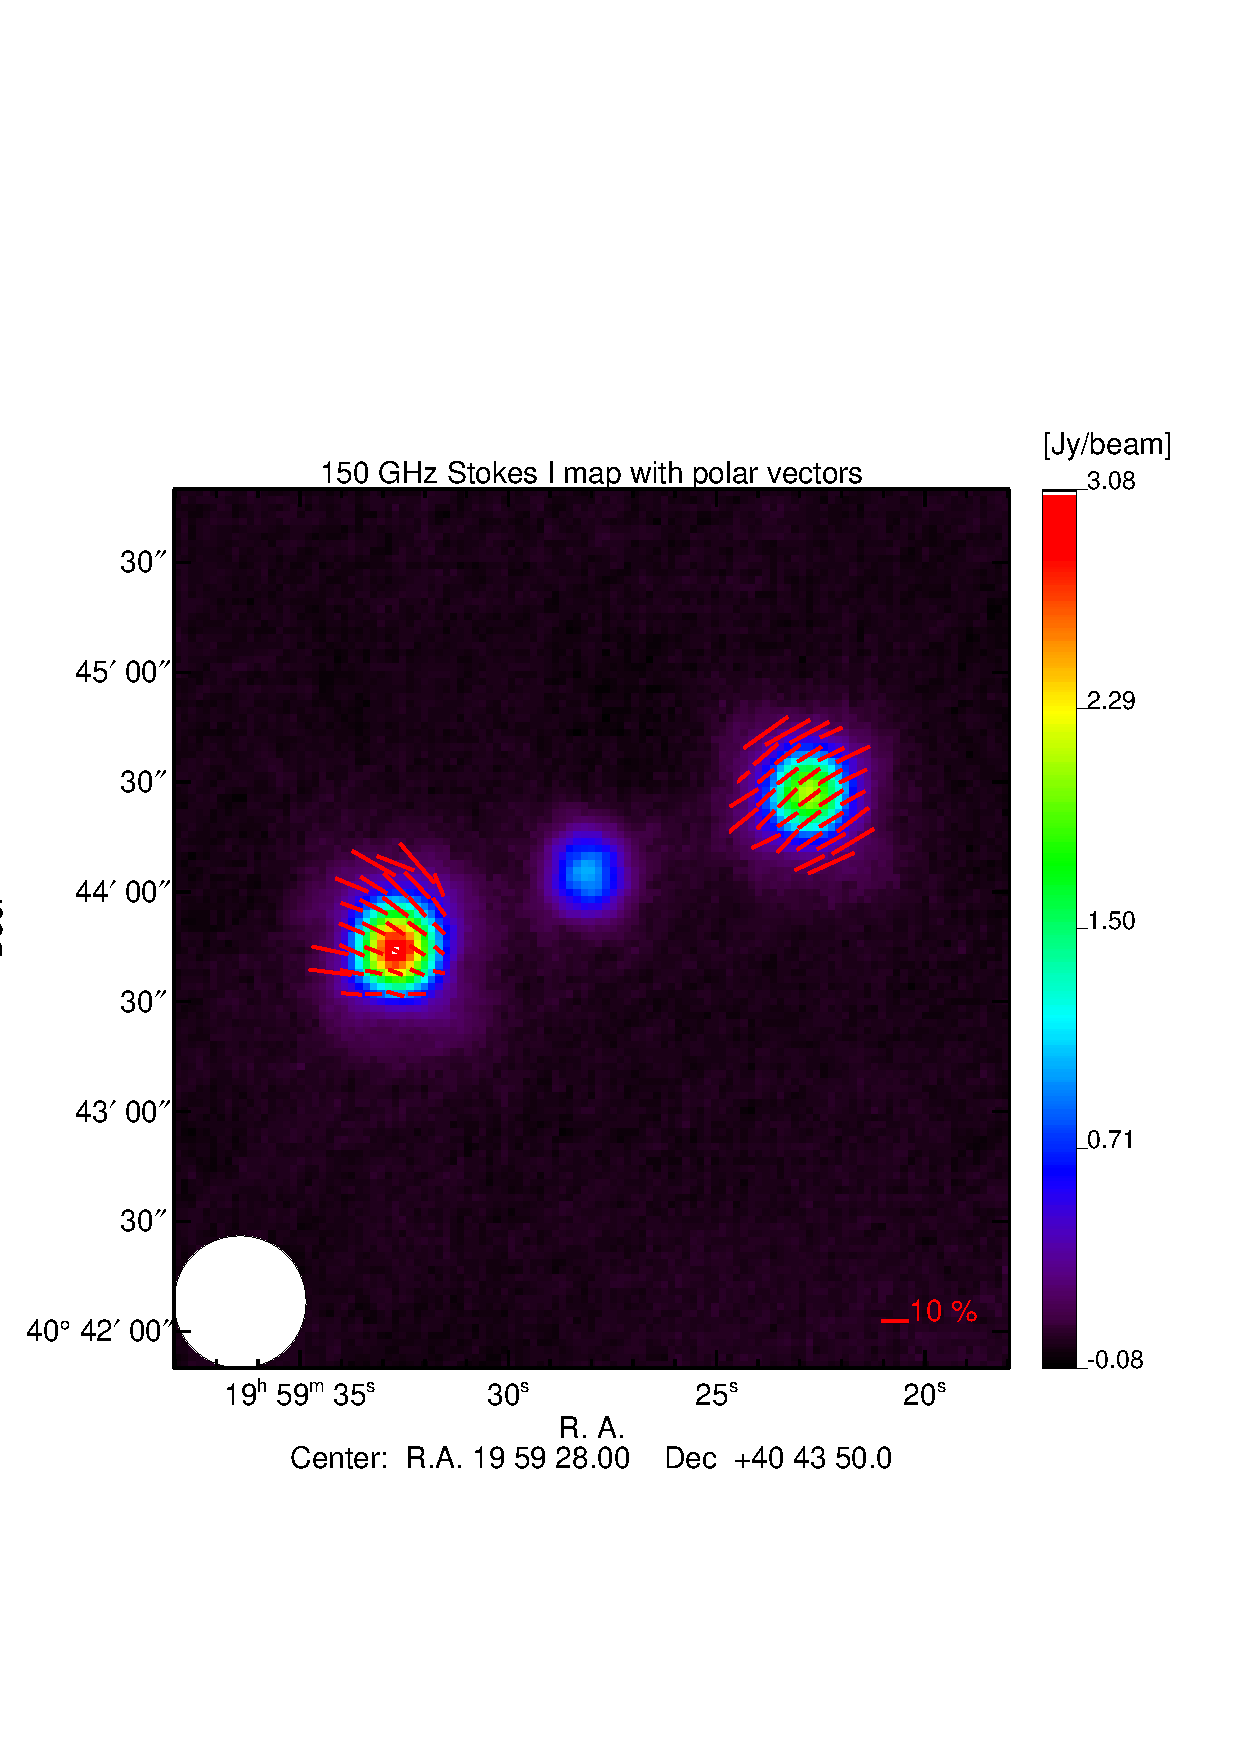
\includegraphics[%
  width=0.33\linewidth,keepaspectratio]{figures/CYGNUSA_I_map_2mm.pdf}
   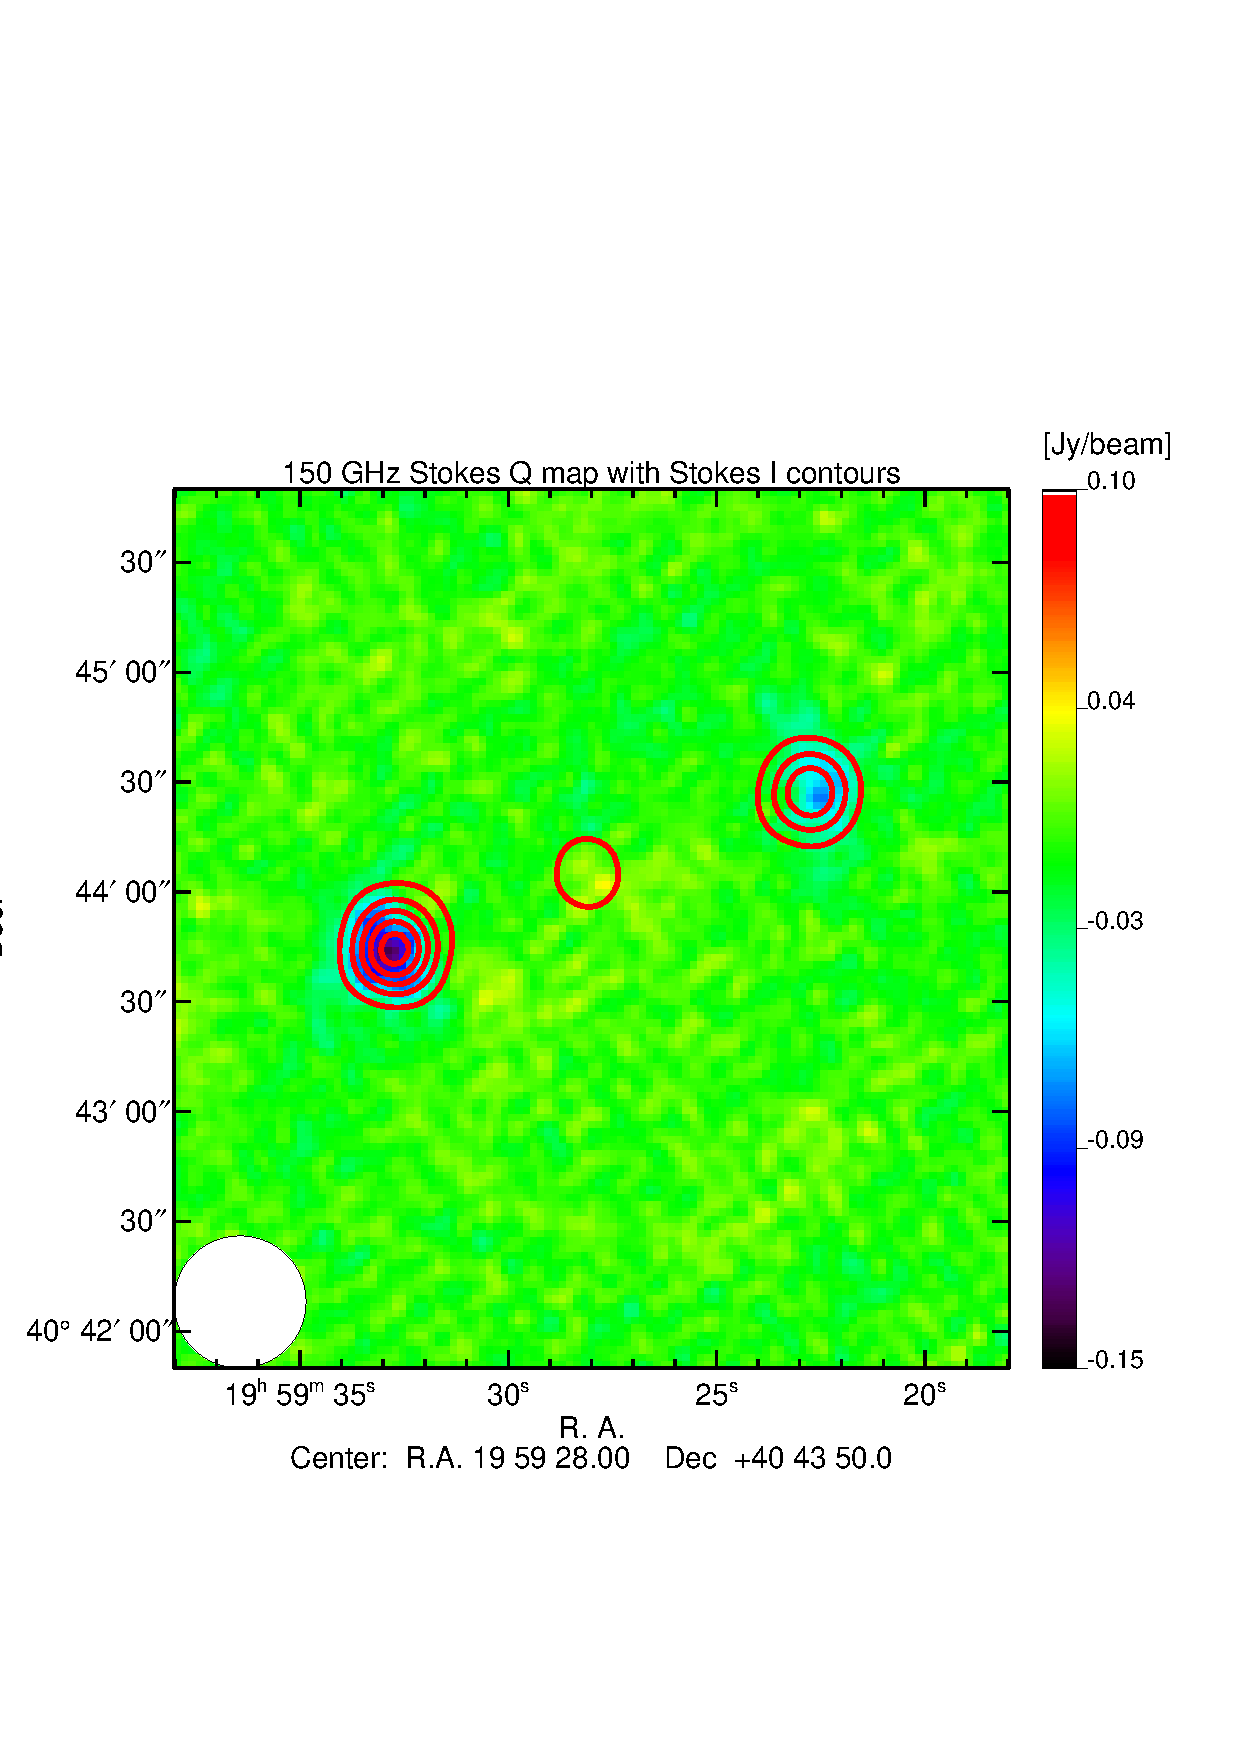
\includegraphics[%
  width=0.33\linewidth,keepaspectratio]{figures/CYGNUSA_Q_map_2mm.pdf}
   \includegraphics[%
  width=0.33\linewidth,keepaspectratio]{figures/CYGNUSA_U_map_2mm.pdf}
   \caption{ Cygnus A Stokes leakage corrected $I$, $Q$ and $U$ maps  at 260 GHz
     (top) and 150 GHz (bottom). polarization vectors are overplotted to the
     intensity maps. The contours in $Q$, $U$ represent the intensity map for
     each frequency. They start from 0.2 Jy/beam$^{-1}$ with steps of 0.2
     Jy/beam$^{-1}$. {\nico on verrait peut etre mieux les vecteurs et les
       contours en blanc ?}}
    \label{cygnusa_maps}
  \end{center}
  \end{figure*}
  
\begin{figure*}
  \begin{center}
    \includegraphics[%
  width=0.33\linewidth,keepaspectratio]{figures/Orion_I_map.pdf}
    \includegraphics[%
  width=0.33\linewidth,keepaspectratio]{figures/Orion_Q_map.pdf}
   \includegraphics[%
  width=0.33\linewidth,keepaspectratio]{figures/Orion_U_map.pdf}
     \includegraphics[%
  width=0.33\linewidth,keepaspectratio]{figures/Orion_I_map_2mm.pdf}
    \includegraphics[%
  width=0.33\linewidth,keepaspectratio]{figures/Orion_Q_map_2mm.pdf}
   \includegraphics[%
  width=0.33\linewidth,keepaspectratio]{figures/Orion_U_map_2mm.pdf}
\caption{ {\it NIKA} Stokes leakage corrected $I$, $Q$ and $U$ maps of Orion
  OMC-1 at 260 GHz (top) and 150 GHz (bottom). polarization vectors are
  overplotted to the intensity maps. The intensity contours overplotted in the
  $Q$ and $U$ maps corresponds to (1, 2, 6, 10, 20, 38) Jy/beam at 260 GHz and
  (2, 4, 6, 8, 10, 14) Jy/beam at 150 GHz. {\nico on voit que la correction de
    leakage a rendu le bruit non gaussien... faudrait soit ameliorer un peu,
    soit le discuter soit changer la table de couleurs...}}
  \label{Orion}
  \end{center}
  \end{figure*}

\begin{figure*}
  \begin{center}
  \includegraphics[%
  width=0.33\linewidth,keepaspectratio]{figures/M87_I_map.pdf}
   \includegraphics[%
  width=0.33\linewidth,keepaspectratio]{figures/M87_Q_map.pdf}
   \includegraphics[%
  width=0.33\linewidth,keepaspectratio]{figures/M87_U_map.pdf}
   \includegraphics[%
  width=0.33\linewidth,keepaspectratio]{figures/M87_I_map_2mm.pdf}
   \includegraphics[%
  width=0.33\linewidth,keepaspectratio]{figures/M87_Q_map_2mm.pdf}
   \includegraphics[%
  width=0.33\linewidth,keepaspectratio]{figures/M87_U_map_2mm.pdf}
   \caption{ \nika\ M87 leakage corrected Stokes  $I$, $Q$ and $U$ maps  at 260 GHz (top) and 150 GHz (bottom). polarization vectors are overplotted to the intensity maps. The contours in $Q$ and $U$ represent the intensity map for each frequency. They start from 0.2 Jy/beam$^{-1}$ with steps of 0.2 Jy/beam$^{-1}$. }
    \label{M87_maps}
  \end{center}
  \end{figure*}
\section{\nika\ polarized observations of compact and extended sources}
\label{sec:extended}
We discuss here observations of compact and extended polarized sources, which
allow us to further validate the quality of the reconstruction of the polarized
sky signal with the \nika\ camera. Special care is taken on the verification of
the validity of the leakage correction algorithm, which can affect the
reconstruction of the direction of polarization across the source. We have
performed observations of different types of sources: Cygnus A, a radio galaxy
consisting of three compact sources; Orion OMC1, a nearby highly polarized
galactic cloud; and M87, an external dusty galaxy.
\subsection{Cygnus A}
Cygnus A is a typical radio galaxy with twin jets of plasma emanating from its
nucleus and forming two extended, radio emitting lobes.  Cygnus A is the most
powerful Fanaroff- Riley II (FRII) radio galaxy in the local environment. It has
been well studied in terms of spatial resolution as it lies at a distance of 227
Mpc. At low radio frequencies, the synchrotron emission from the two giant lobes
dominate \citep{1974MNRAS.166..305H}. At higher frequencies the hotspots
(working surfaces in the lobes) and the galaxy core become more prominent. The
southern and northern hotspots are at 50 and 70 arcsec from the core,
respectively.  The complex structure of Cygnus A can be well explained by
assuming that it consists of two components, which are polarized in opposite
directions and of an unpolarized core (\cite{1967ApJ...150L..15S}, \cite{1966SvA....10..214S},
\cite{1968ApJ...151...53M}).

The leakage corrected \nika\ Stokes $I$, $Q$, and $U$ maps of Cygnus A at 260
(top row) and 150 (bottom row) GHz are presented in Figure~\ref{cygnusa_maps}.
{\nico On} the intensity maps the polarization vectors are overplotted in
yellow. {\nico On} the $Q$ and $U$ maps intensity contours are also represented in
black.  As expected, {\nico on} the intensity maps at 1.25 and 2.05 mm we clearly
observe three compact sources {\nico that correspond} to the core and the two lobes.
By contrast the polarization maps show only two sources at the position of the
intensity lobes. At the position of the core the polarized signal is {\nico consistant}
with zero, revealing the low level of instrumental polarization. The
polarization of the jets shows opposite orientation as expected.
%As expected, the
%two hot spots and the galaxy core dominate the signal at the {\it NIKA}
%frequencies. The peak flux of the $I$ map is $\sim$ 1.7 Jy/beam and $\sim$ 3 Jy/beam at 260 GHz and 150 GHz, respectively. 
%The leakage maps found for this source are shown in Fig. \ref{cygnusa_leakage}, the effect is comparable to the quasar leakage effect, for Cygnus A appears as a compact source at {\it NIKA} frequencies. 
%The polarization intensity at both frequencies is shown in Fig. \ref{cygnusa_ipol}. In Fig. \ref{cygnusa_vector} we show the Stokes vector $I$ with the vectors indicating the orientation of the polarization angle. 
\subsection{Orion OMC-1}
The Orion Molecular Cloud (OMC-1) is the closest site of OB star formation. The
KL Nebula is the flux peak from far infrared to millimeter wavelengths on the
OMC-1 ``ridge" \citep{schle1998}.  A sub-millimeter peak, ``KHW" with equal mass
but lower dust temperature, is found 90 arcsec south of KL along the ridge
\citep{KHW1982}. At KL and KHW, the percent polarization increases with
wavelength \citep{schle1998}.  Figure~\ref{Orion} presents the \nika\ leakage
corrected Stokes $I$, $Q$ and $U$ maps of Orion OMC-1 at 260 (top) and 150
(bottom) GHz.  The polarization vectors are over-plotted in the intensity maps,
showing the polarization intensity and orientation. The peak flux of the OMC-1
emission is about 45.8 Jy/beam and 14 Jy/beam at 260 GHz and 150 GHz,
respectively. The size of the map is 8 x 8 arcminutes obtained by the
co-addition of 18 maps for a total observational time of {\nico about} 5h. The
sensitivities measured on the maps are {\nico respectively} 5 and 2.5 mJy
$s^\frac{1}{2}$ in total $I$ at 260 and 150 GHz {\nico 150 or 160 ?}).  The
  orientation of the polarization vectors is consistent between the 260 and 150
  {\nico 150 or 160 ?} GHz maps, confirming that {\nico the} observed {\nico
    polarization} has the same physical
  origin. The most polarized structures are not aligned with the intensity
  peaks. The polarization vectors are well aligned following the intensity
  structures across the source suggesting a strong ordered magnetic field. These
  structures and filaments are consistent with OMC-1 observations performed with
  SCUPOL \citep{scubapol} at 850 $\mu$m.  Previous observations at 1.3 mm
  performed by \citep{leach1991} show that from the KL position, the average
  polarization rises to 4\%-5\% while at KL, the polarization drops to 2.7\%.
  Averaging across the KL nebula on \nika\ Orion maps at 260 GHz (1.25 mm) we
  find that the angle and degree of polarization are $\chi$ = (23.19 $\pm$
  1.24)$^\circ$ and $p$ = (2.7 $\pm$ 0.1) $\%$.  Then, for the KHM region we
  find $\chi$ = (18.7 $\pm$ 0.7)$^\circ$ and $p$ = (4.6 $\pm$ 0.2)
  $\%$. Consistent results are found at 150 GHz (2.05 mm).
%$\chi$ = [19.07 $\pm$ 1.15(stat) $\pm$ 1.8(syst)]$^\circ$ and $p$ = (2.6 $\pm$ 0.1) $\%$ at 150 GHz. 
%At the KHM region we find $\chi$ = (18.7 $\pm$ 0.7 stat) $\pm$ 1.8(syst)) $^\circ$ and $p$ = (4.6 $\pm$ 0.2) $\%$ and $\chi$ = [18.0 $\pm$ 0.6 stat) $\pm$ 1.8(syst)]$^\circ$ and $p$ = (4.7 $\pm$ 0.2) $\%$ at 260 and 150 GHz, respectively.
These results are {\nico also} in rough agreement with POLKA observations {\nico
  who} found a polarization angle of $32.8\pm7.6^\circ$ \citep{polka_apex}.
\begin{table*}
\begin{center}
\caption{Summary on KL nebula polarization degree and angle results reported by previous experiments and \nika\ .}
\begin{tabular}{cccccccccccc}
\hline
\hline
  & \multicolumn {3} {c} {p [$\%$]} & \multicolumn {3} {c} {$\chi$ [$^\circ$]} \\
\hline
& POLKA  & SCUPOL  &  \nika\  & POLKA  & SCUPOL   &  \nika\ \\
 \hline
 & [870 $\mu$ m] &  [850 $\mu$ m]  &  [1.25 - 2.05 mm]  &  [870 $\mu$ m] &  [850 $\mu$ m]  &  [1.25 - 2.05 mm] \\
 \hline
 KL & 0.7 $\pm$ 0.2 & 0.7 $\pm$ 0.1 & (2.7 $\pm$ 0.1) - (2.6 $\pm$ 0.1) &  32.8 $\pm$ 7.6 & 40.8 $\pm$ 5.4 & [23.19 $\pm$ 1.24] - [19.07 $\pm$ 1.15] \\ 
\hline
\hline
\end{tabular}
\label{tab:tab_orion}
\end{center}
\end{table*}
%The leakage maps found for this source represented in fig. \ref{Orion_leakage} show a reduced leakage effect compared to point source polarization degree. In fig. \ref{orion_vector} we show the Stokes vector $I$ with the vectors indicating the orientation of the polarization angle.
%In Fig. \ref{Orion_scuba} we show the maps of Orion OMC-1 obtained by SCUPOL instrument \citep{scubapol} at 850 $\mu$m. The contours represent the {\it NIKA} map obtained at 1.25 mm. We observe a bit shift between the two maps may be due to some pointing error in the specific observation session. 
%If we compare the polarization intensity IPOL in Fig. \ref{Orion_scuba} on right with the polarization intensity  $IPOL$ = $\sqrt{Q^2 + U^2}$ obtained by {\t NIKA} observation in Fig. \ref{Orion_ipol} there is a consistency in the shape of the polarized regions. 
%\begin{figure}
%  \begin{center}
%    \includegraphics[%
%  width=1.\linewidth,keepaspectratio]{figures/NIKAvsScuba.pdf}
%  \caption{ \NIKA\ Stokes $I$ at 260 GHz with SCUPOL map contours at 850 $\mu m$. The \NIKA\ map is shifted by $\sim$ 10 arcsec to match the SCUPOL map.}
%  \label{Orion_scuba}
%  \end{center}
 % \end{figure} 
\subsection{M87}
M87, also designated as 3C274, or NGC 4486, or Virgo A, is a giant elliptical
galaxy \citep{dev76} located near the core of the Virgo cluster.  Its nucleus is
a radio and X-ray source {\nico **} from which emanates an optical jet.  M87 is
estimated to be about 16 Mpc from {\nico **} Earth \citep{mou80}. The core and
{\nico the} jet can be seen at all {\nico wavelengths} from radio to X-rays.
%Radio galaxies serve as a probe of their environments, providing means
%to study the pressure, density, temperature, and magnetic strength, {\it
%etc.} of the extragalactic medium (IGM) or intra-cluster
%medium (ICM). 
%The galaxy M87 is more studied at lower frequencies than the {\it NIKA} ones in order to study the physics of the filaments, the polarization 
%degrees of the filaments are very high near the limit of synchrotron 
%emission at this frequencies. At {\it NIKA} frequencies the galaxy appears with its core and the surrounding lobes. 
Figure~\ref{M87_maps} presents the \nika\ leakage corrected Stokes $I$, $Q$ and
$U$ maps at 260 (top) and 150 (bottom) GHz. The polarization vectors are
overplotted in yellow {\nico on} the intensity maps representing both the degree and
orientation of polarization. The peak flux of the $I$ map is $\sim$ 0.6 Jy/beam
$\sim$ 1.5 Jy/beam at 260 GHz and 150 GHz, respectively. This confirms the fact
that the M87 emission is dominated by synchrotron. The polarization vectors are
well aligned following the contours of the intensity contours. They suggest the
existence of a large scale ordered magnetic field in the radio lobes of M87.
%The polarized intensity at 150 GHz shown in Fig. \ref{M87_ipol} suggests a synchrotron emission of the M87 lobes.  The polarized emission at 260 GHz is quite weak. 
% Fig. \ref{m87_vector} show the Stokes vector $I$ with the vectors indicating the orientation of the polarization angle at both frequencies.  T
%The hot spots present a spectral index (right map on the row) in
%the range -1.5 to -2.0, which is consistent with synchrotron emission but
%steeper than the value found by \citet{1998MNRAS.301..935R}, which is $\sim
%-1$. The galaxy core shows a flatter spectrum from -0.6 to -1.0, which is
%consistent with previous estimates from \citet{1999IAUS..194..179L}.
 \section{Conclusions}
This paper has presented the first ever polarization measurements with kinetic
inductance detectors (KIDs) {\nico in your face! :)}. For these measurements we
have adopted a simplified polarization system consisting of an achromatic
continuously rotating HWP {\nico at about 3~Hz}, an analyser and arrays of KIDs
not sensitive to polarization.  The fast modulation of the input polarization
signal with the HWP has allowed us to significantly reduce the atmospheric
emission in the polarized signal. Instrumental polarization in the form of
intensity to polarization leakage has been observed at the level of 3 and 2\%
peak to peak for point like and extended sources respectively.  We have successfully
developed an algorithm to correct for this systematic effect and subtract it to
better than {\nico XXX}.

{\nico We have observed 3C286, a quasar used as standard polarization calibrator
  in the literature and have found a total flux, a polarization degree and
  orientation in agreement with existing data, thus establishing the accuracy of
  our system and analysis.} These results have been confirmed and extended with
observations of compact and extended sources such as Cygnus A, OMC-1 and
M87. These \nika\ observations have revealed that polarized vectors align well
with the intensity structures indicating the presence of well ordered magnetic
fields.
 %A systematic leakage effect of total intensity into polarization shows up at the 3\% level for point sources and 2\% for extended sources. 
% We have been able to correct for it using calibration scan on Uranus on all observations shown in the section \ref{sec:polar_pipe}.
 \nika\ has been a successful test-bench for the \nikad\ camera, which shares
 the same polarization system (fast continuously rotating HWP and analyser).
 \nikad\ observes the sky at the same {\nico **} frequencies with ten times more
 detectors and a Field of View (Fov) of 6.5 arcminutes.  The \nikad\ camera
 has been installed at the IRAM 30 meter telescope in Spain on October 2015
 {\nico to enter its commissioning phase. In \nikad\ though, polarization
   capabilities will be limited to the 260~GHz channel. This first technical
   paper shows the potentialities of \nikad\ in terms if polarimetric
   measurements and its ability to provide advances in the field of Galactic
   emission and interactions with the magnetic field... bla bla... a reprendre
   en mieux, je dois partir. Ne pas mentionner d'ouverture au public pour le moment...}



%%and
%% it will be opened to public observations late 2016. The {\it NIKA}2
%% capabilities are restricted to the 260 GHz channel,
%% %{\it NIKA}2 has polarization capability at 260 GHz; the warm rotating HWP is placed in front of the {\it NIKA}2 cryostat and and the polarizer is mounted in the 100 mK stage of the cryostat splitting the two orientations of the linear polarization on two matrix of thousands of pixels.
%
which will provide high angular resolution observations of Galactic regions helping the understanding of the magnetic fields role in star formation process. 

\bibliography{biblio}
% \begin{figure*}
%  \begin{center}
%   \includegraphics[%
%    width=0.24\linewidth,keepaspectratio]{figures/Orion_IQ_1mm.pdf}
%    \includegraphics[%
%  width=0.24\linewidth,keepaspectratio]{figures/Orion_IU_1mm.pdf}
%  \includegraphics[%
%    width=0.24\linewidth,keepaspectratio]{figures/Orion_IQ_2mm.pdf}
%    \includegraphics[%
%  width=0.24\linewidth,keepaspectratio]{figures/Orion_IU_2mm.pdf}
%  \caption{ From left to right Orion OMC-1 intensity to polarization leakage maps $IQ$, $IU$ at 260 GHz and at 150 GHz.}
%  \label{Orion_leakage}
%  \end{center}
%  \end{figure*}
  

%\begin{figure*}
%  \begin{center}
%        \includegraphics[%
%  width=0.4\linewidth,keepaspectratio]{figures/Orion_ipol_1mm.pdf}
%     \includegraphics[%
%  width=0.4\linewidth,keepaspectratio]{figures/Orion_ipol_2mm.pdf}
%     \caption{ polarization intensity maps at 260 GHz (left) and 150 GHz (right) of the molecular cloud Orion OMC-1. }
%    \label{Orion_ipol}
%  \end{center}
%  \end{figure*}



 % M87
  
    
  % \begin{figure*}
 % \begin{center}
  % \includegraphics[%
  %  width=0.24\linewidth,keepaspectratio]{figures/M87_IQ_1mm.pdf}
   % \includegraphics[%
  %width=0.24\linewidth,keepaspectratio]{figures/M87_IU_1mm.pdf}
  %\includegraphics[%
 %   width=0.24\linewidth,keepaspectratio]{figures/M87_IQ_2mm.pdf}
   % \includegraphics[%
 % width=0.24\linewidth,keepaspectratio]{figures/M87_IU_2mm.pdf}
  %\caption{ From left to right M87 intensity to polarization leakage maps $IQ$, $IU$ at 260 GHz and at 150 GHz.}
  %\label{M87_leakage}
 % \end{center}
 % \end{figure*}
  
  %\begin{figure*}
  %\begin{center}
  %\includegraphics[%
 % width=0.48\linewidth,keepaspectratio]{figures/M87_ipol_1mm.pdf}
 % \includegraphics[%
 % width=0.48\linewidth,keepaspectratio]{figures/M87_ipol_2mm.pdf}
  %  \caption{ M87 polarization intensity maps at 260 GHz (left) and 150 GHz (right). }
   %   \label{M87_ipol}
  %\end{center}
  %\end{figure*} 
 
  % Cygnusa
  

  
 %  \begin{figure*}
 % \begin{center}
 % \includegraphics[%
 %  width=0.24\linewidth,keepaspectratio]{figures/Cygnus_A_IQ_1mm.pdf}
 %   \includegraphics[%
 % width=0.24\linewidth,keepaspectratio]{figures/Cygnus_A_IU_1mm.pdf}
 %\includegraphics[%
 %   width=0.24\linewidth,keepaspectratio]{figures/Cygnus_A_IQ_2mm.pdf}
 %   \includegraphics[%
 % width=0.24\linewidth,keepaspectratio]{figures/Cygnus_A_IU_2mm.pdf}
 % \caption{ From left to right Cygnus A intensity to polarization leakage maps $IQ$, $IU$ at 260 GHz and at 150 GHz.}
 % \label{cygnusa_leakage}
%  \end{center}
%  \end{figure*}
  
%  \begin{figure*}
%  \begin{center}
%  \includegraphics[%
%  width=0.48\linewidth,keepaspectratio]{figures/Cygnus_ipol_1mm_NIKA.pdf}
%  \includegraphics[%
%  width=0.48\linewidth,keepaspectratio]{figures/Cygnus_ipol_2mm_NIKA.pdf}
%   \caption{ Cygnus A polarization intensity maps at 260 GHz (left) and 150 GHz (right). }
%      \label{cygnusa_ipol}
%  \end{center}
%  \end{figure*} 
 
  % Projection of vectors------------------
  
% \begin{figure*}
%  \begin{center}
%  \includegraphics[%
%  width=0.42\linewidth,keepaspectratio]{figures/map_I_1mm_vector_M87.pdf} 
%  \includegraphics[%
%  width=0.42\linewidth,keepaspectratio]{figures/map_I_2mm_vector_M87.pdf} 
%    \caption{ M87 Stokes vector $I$ intensity with polarization vectors at 260 GHz (left) and 150 GHz (right).}
%  \label{m87_vector}
%   \end{center}
%  \end{figure*}

%\begin{figure*}
%  \begin{center}
%  \includegraphics[%
%  width=0.42\linewidth,keepaspectratio]{figures/Cygnusa_map_I_1mm_vector.pdf} 
%  \includegraphics[%
%  width=0.42\linewidth,keepaspectratio]{figures/Cygnusa_map_I_2mm_vector.pdf} 
%    \caption{ Cygnus A Stokes vector $I$ intensity with polarization vectors at 260 GHz (left) and 150 GHz (right).}
%	\label{cygnusa_vector}
%   \end{center}
%  \end{figure*}

 
  
  %-----------------------------------------------------
  


%\pagebreak

        
\end{document}
